% #############################################################################
% This is the MAIN DOCUMENT of the IST-Thesis MSc TEMPLATE.
% The content for the IST-Thesis MSc is to be written in separate documents
% located in the folder ./Chapters
%         Aknowledgments.tex
%         Abstract.tex
%         KeyWords.tex
%         Resumo.tex
%         PalavrasChave.tex
%         Acronyms.tex
%         Front_Cover.tex
%         Chapter_1.tex ....Chapter_2 .....
%         ApendixA.tex ... ApendixB.tex...
% -----------------------------------------------------------------------------
% The class "istulthesis" is based on the standard LaTeX 'report' class.
% It can be used for Instituto Superior Tecnico thesis, as it follows the 
% regulations published by the Scientific Council of IST.
% The class defines the document style. 
% IST requires the thesis to be written in Arial or similar. 
% Two arguments in '\documentclass' allow you to define the thesis font: 
% 'Helvetica' and 'AvantGarde', which transforms 
% the default LaTeX font into Helvetica or AvantGarde, respectively.
% #############################################################################
% The document is automatically set for english or portuguese by just selecting
% the MAIN LANGUAGE in file 'IST-Thesis-MSc-Preamble_commands.tex' 
% #############################################################################
% IST-Thesis-MSc
% Version 1.0, August 2014
% BY: Rui Santos Cruz, rui.s.cruz@tecnico.ulisboa.pt
% #############################################################################
% !TEX root = ./main.tex
% -----------------------------------------------------------------------------
%
\documentclass[defaultstyle,10pt,Helvetica]{istulthesis}

% -----------------------------------------------------------------------------
% The Preamble document contains all the necessary Packages for typesetting
% Modify it to suit your needs
% -----------------------------------------------------------------------------
% #############################################################################
% Preamble for IST-Thesis-MSc in English or Portuguese
% Required Packages and commands
% --> Please Choose the MAIN LANGUAGE for the Thesis in package BABEL (below)
% !TEX root = ./main.tex
% #############################################################################
% IST-Thesis-MSc
% Version 1.0, August 2014
% BY: Rui Santos Cruz, rui.s.cruz@tecnico.ulisboa.pt
% #############################################################################
%
% -----------------------------------------------------------------------------
% PACKAGE ucs:
% -----------------------------------------------------------------------------
% The 'ucs' package provides support for using UTF-8 in LaTeX documents. 
% However in most situations it is not required.
\usepackage{ucs}

% -----------------------------------------------------------------------------
% PACKAGE utf8x:
% -----------------------------------------------------------------------------
% The 'utf8x' package contains support for using UTF-8 as input encoding. 
\usepackage[utf8x]{inputenc}

% -----------------------------------------------------------------------------
% PACKAGE babel:
% -----------------------------------------------------------------------------
% The 'babel' package may correct some hyphenation issues of LaTeX. 
% Select your MAIN LANGUAGE for the Thesis with the 'main=' option.
% 
\usepackage[main=english,portuguese]{babel}

% -----------------------------------------------------------------------------
% PACKAGE iflang:
% -----------------------------------------------------------------------------
% The 'iflang' package is used to help determine the language being used. 
\usepackage{iflang}

% -----------------------------------------------------------------------------
% PACKAGE scrbase:
% -----------------------------------------------------------------------------
% The 'scrbase' package is used to help redefining document structure.
\usepackage{scrbase}

% -----------------------------------------------------------------------------
% PACKAGE enumerate:
% -----------------------------------------------------------------------------
%For enhanced enumeration of lists
\usepackage{enumerate}

% -----------------------------------------------------------------------------
% PACKAGE latexsym:
% -----------------------------------------------------------------------------
% Defines additional latex symbols. 
% May be required for thesis with many math symbols.
%\usepackage{latexsym}

% -----------------------------------------------------------------------------
% PACKAGE mathtools, amsmath, amsthm, amssymb, amsfonts:
% -----------------------------------------------------------------------------
% These packages are typically required. 
% Among many other things they add the possibility to put symbols in bold
% by using \boldsymbol (not \mathbf); defines additional fonts and symbols;
% adds the \eqref command for citing equations.
\usepackage{mathtools, amsmath, amsthm, amssymb, amsfonts}

% -----------------------------------------------------------------------------
% PACKAGE multirow, colortbl, ctable, longtable:
% -----------------------------------------------------------------------------
% These packages are most usefull for advanced tables. 
% 'multirow' allows to join rows throuhg the command \multirow which works
% similarly with the command \multicolumn.
% The 'colortbl' package allows to color the table (foreground and background)
% The 'ctable' package provides commands to easily typeset centered or left or
% right aligned tables.
% The package 'booktabs' provide some additional commands to enhance
% the quality of tables
% The 'longtable' package is only required when tables extend beyond the length
% of one page, which typically does not happen and should be avoided
\usepackage{multirow}
\usepackage{colortbl}
\usepackage{ctable}
\usepackage{booktabs}
\usepackage{longtable}

% -----------------------------------------------------------------------------
% PACKAGES graphicx, subfigure:
% -----------------------------------------------------------------------------
% The package 'graphicx' supports formats PNG and JPG.
% Package 'subfigure' allows to place figures within figures with own caption. 
% For each of the subfigures use the command \subfigure.
\usepackage{graphicx}
\usepackage[hang,small,bf,tight]{subfigure}

% -----------------------------------------------------------------------------
% PACKAGE caption:
% -----------------------------------------------------------------------------
% The 'caption' package offers customization of captions in floating 
% environments such figure and table
% \usepackage[hang,small,bf]{caption}
\usepackage[format=hang,labelfont=bf,font=small]{caption} 
% the following customization adds vertical space between caption and the table
\captionsetup[table]{skip=10pt}

% -----------------------------------------------------------------------------
% PACKAGE algorithmic, algorithm, algorithm2e:
% -----------------------------------------------------------------------------
% These packages are required if you need to describe an algorithm.
% The preference is for using 'algorithm2e'
%\usepackage{algorithmic}
%\usepackage[chapter]{algorithm}
\usepackage[ruled,vlined,algochapter,norelsize,\languagename]{algorithm2e}

% -----------------------------------------------------------------------------
% PACKAGE listings
% -----------------------------------------------------------------------------
% These packages are required if you need to list code snippets.
\usepackage{listings}
% Nicely syntax highlighted m-code in LaTeX documents with stylefile mcode.sty
% http://www.mathworks.com/matlabcentral/fileexchange/8015-m-code-latex-package
\usepackage[numbered]{./tables_and_code/mcode}

% -----------------------------------------------------------------------------
% Re-define listings captions and titles based on language.
\newcaptionname{portuguese}{\lstlistingname}{Listagem} % Listings CAPTIONS
\newcaptionname{portuguese}{\lstlistlistingname}{Listagens} % LIST of LISTINGS

% -----------------------------------------------------------------------------
% PACKAGES xcolor, color
% -----------------------------------------------------------------------------
% These packages are required if you need to list code snippets.
\usepackage{xcolor}
\usepackage{color}
% The following special color definitions are used in the IST Thesis
\definecolor{forestgreen}{RGB}{34,139,34}

\definecolor{orangered}{RGB}{239,134,64}
\definecolor{lightred}{rgb}{1,0.4,0.5}
\definecolor{orange}{rgb}{1,0.45,0.13}	

\definecolor{darkblue}{rgb}{0.0,0.0,0.6}
\definecolor{lightblue}{rgb}{0.1,0.57,0.7}

\definecolor{gray}{rgb}{0.4,0.4,0.4}
\definecolor{lightgray}{rgb}{0.95, 0.95, 0.95}
\definecolor{darkgray}{rgb}{0.4, 0.4, 0.4}
\definecolor{editorGray}{rgb}{0.95, 0.95, 0.95}
\definecolor{editorOcher}{rgb}{1, 0.5, 0} % #FF7F00 -> rgb(239, 169, 0)
\definecolor{chaptergrey}{rgb}{0.6,0.6,0.6}

\definecolor{editorGreen}{rgb}{0, 0.5, 0} % #007C00 -> rgb(0, 124, 0)

\definecolor{olive}{rgb}{0.17,0.59,0.20}
\definecolor{brown}{rgb}{0.69,0.31,0.31}

\definecolor{purple}{rgb}{0.38,0.18,0.81}

% -----------------------------------------------------------------------------
% PACKAGE setspace:
% ----------------------------------------------------------------------------
% Pro­vides sup­port for set­ting the spac­ing be­tween lines in a doc­u­ment. 
% Pack­age op­tions in­clude sin­glespac­ing, one­half­s­pac­ing, and dou­blespac­ing. 
% Al­ter­na­tively the spac­ing can be changed as re­quired with:
% \sin­glespac­ing, \one­half­s­pac­ing, and \dou­blespac­ing com­mands
\usepackage{setspace}

% -----------------------------------------------------------------------------
% PACKAGE paralist
% -----------------------------------------------------------------------------
% This package provides the 'inparaenum' environment for inline lists
\usepackage{paralist}

% -----------------------------------------------------------------------------
% PACKAGE cite:
% -----------------------------------------------------------------------------
% The 'cite' package will result in citation numbers being automatically
% sorted and properly "ranged". i.e.,
% [1], [2], [5]--[7], [9]
\usepackage{cite}

\usepackage{float}

% -----------------------------------------------------------------------------
% PACKAGE acronym:
% -----------------------------------------------------------------------------
% The package 'acronym' garantees that all acronyms definitions are 
% given at the first usage. 
% IMPORTANT: do not use acronyms in titles/captions; otherwise the definition 
% will appear on the table of contents.
\usepackage[printonlyused]{acronym}

% -----------------------------------------------------------------------------
% PACKAGE hyperref
% -----------------------------------------------------------------------------
% Set links for references and citations in document
\usepackage{hyperref}
% pre-configuration of hyperref
\hypersetup{ colorlinks=true,
             citecolor=cyan,
             linkcolor=darkgray,
             urlcolor=teal,
             breaklinks=true,
             bookmarksnumbered=true,
             bookmarksopen=true,
             pdftitle=\@title, % THESIS TITLE
             pdfauthor=\@author,  % YOUR NAME
             pdfcreator=\@author,   % YOUR NAME
}

% -----------------------------------------------------------------------------
% PACKAGE url:
% -----------------------------------------------------------------------------
% Provides better support for handling and breaking URLs.
\usepackage{url} 

% #############################################################################
% GLOBAL FORMATTING OF THE THESIS DOCUMENT before using FANCY stuff
% Set paragraph counter to alphanumeric mode
\renewcommand{\theparagraph}{\Alph{paragraph}~--}

\hoffset 0in
\voffset 0in
\oddsidemargin 0 cm
\evensidemargin 0 cm
\marginparsep 0in
\topmargin -0.25cm
\textwidth 16 cm
\textheight 22.4 cm

% -----------------------------------------------------------------------------
% PACKAGE fancyhdr:
% -----------------------------------------------------------------------------
% The fancyhdr macro package allows to customize page headers and footers.
\usepackage{fancyhdr}
\pagestyle{fancy}

\renewcommand{\chaptermark}[1]{\markboth{\thechapter.\ #1}{}}
\renewcommand{\sectionmark}[1]{\markright{\thesection\ #1}}

\fancyhead{}
\renewcommand{\headrulewidth}{0.0pt}
\renewcommand{\footrulewidth}{0.0pt}
\addtolength{\headheight}{2pt} % make space for the rule

\fancypagestyle{plain}{%
   \fancyhead{} % get rid of headers
   \renewcommand{\headrulewidth}{0pt} % and the line
   \renewcommand{\footrulewidth}{0pt}
}
\fancypagestyle{blank}{%
   \fancyhf{} % get rid of headers and footers
   \renewcommand{\headrulewidth}{0pt} % and the line
   \renewcommand{\footrulewidth}{0pt}
}
\fancypagestyle{abstract}{%
   \fancyhead{}
   \renewcommand{\headrulewidth}{0pt}
   \renewcommand{\footrulewidth}{0.0pt}
}
\fancypagestyle{document}{%
	\fancyhead{}
	\renewcommand{\headrulewidth}{0.5pt}
	\renewcommand{\footrulewidth}{0.5pt}
	\addtolength{\headheight}{2pt} % make space for the rule
}

\setcounter{secnumdepth} {5}
\setcounter{tocdepth} {5}

\renewcommand{\thesubsubsection}{\thesubsection.\Alph{subsubsection}}

\renewcommand{\subfigtopskip}{0.3 cm}
\renewcommand{\subfigbottomskip}{0.2 cm}
\renewcommand{\subfigcapskip}{0.3 cm}
\renewcommand{\subfigcapmargin}{0.2 cm}


% -----------------------------------------------------------------------------
% PACKAGE minitoc:
% -----------------------------------------------------------------------------
% Package 'minitoc' creates a mini-table of contents (a “minitoc”) at 
% the beginning of each chapter of a document.
% This packages are required for the \fancychapter configuration
\usepackage{minitoc}
\setcounter{minitocdepth}{1}
\setlength{\mtcindent}{24pt}
\renewcommand{\mtcfont}{\small\rm}
\renewcommand{\mtcSfont}{\small\bf}
\renewcommand*{\kernafterminitoc}{\kern0.\baselineskip\kern0.ex}
\mtcselectlanguage{\languagename} 

% Now prepare the MINITOC
\def\boxedverbatim{%
  \def\verbatim@processline{%
    {\setbox0=\hbox{\the\verbatim@line}%
    \hsize=\wd0 \the\verbatim@line\par}}%
  \@minipagetrue%%%DPC%%%
  \@tempswatrue%%%DPC%%%
  \setbox0=\vbox\bgroup\vspace*{0.2cm}\footnotesize\verbatim
}
\def\endboxedverbatim{%
  \endverbatim
  \unskip\setbox0=\lastbox %%%DPC%%%
  \hspace*{0.2cm}
  \vspace*{-0.2cm}
  \egroup
  \fbox{\box0}% <<<=== change here for centering,...
}

% Now prepare the CHAPTER Number
\newcommand*{\chapnumfont}{%
%   \usefont{T1}{\@defaultcnfont}{b}{n}\fontsize{100}{130}\selectfont%
  \usefont{T1}{pbk}{b}{n}
  \fontsize{150}{130}
  \selectfont
  \color{chaptergrey}
}
\makeatletter
\def\@makechapterhead#1{%
  \vspace*{50\p@}%
  {\parindent \z@ \raggedright \normalfont
    {\chapnumfont\ifnum \c@secnumdepth >\m@ne
%         \huge\bfseries \@chapapp\space \thechapter
        \raggedleft\bfseries \thechapter
        \par\nobreak
        \vskip 20\p@
    \fi}
    \interlinepenalty\@M
    {\raggedleft\Huge \bfseries #1\par\nobreak}
    \vskip 40\p@
  }}
\makeatother

% Now put it all together as a command \fancychapter
\newcommand{\fancychapter}[1]{\chapter{#1}\vfill\minitoc\pagebreak}

% #############################################################################
% ADDITIONAL COMMANDS AND CONFIGURATIONS
% #############################################################################
% This commmand allows to place horizontal lines with a custom width... 
% replaces the standard hline command
\newcommand{\hlinew}[1]{%
  \noalign{\ifnum0=`}\fi\hrule \@height #1 \futurelet
   \reserved@a\@xhline}
   
% -----------------------------------------------------------------------------
% This command defines some marks... USEFUL FOR TABLES.
\def\Mark#1{\raisebox{0pt}[0pt][0pt]{\textsuperscript{\footnotesize\ensuremath{\ifcase#1\or *\or \dagger\or \ddagger\or%
    \mathsection\or \mathparagraph\or \|\or **\or \dagger\dagger%
    \or \ddagger\ddagger \else\textsuperscript{\expandafter\romannumeral#1}\fi}}}}

% -----------------------------------------------------------------------------
% The following configurations are used for LISTINGS of certain languages

\lstdefinestyle{XML} {
	language=XML,
	extendedchars=true, 
	breaklines=true,
	breakatwhitespace=true,
	emph={},
	emphstyle=\color{red},
	basicstyle=\small,
	xleftmargin=17pt,
	columns=fullflexible,
	commentstyle=\color{gray}\upshape,
	morestring=[b][\color{brown}]",
	morecomment=[s]{<?}{?>},
	morecomment=[s][\color{forestgreen}]{<!--}{-->},
	keywordstyle=\color{orangered},
	stringstyle=\ttfamily\color{black},
	% stringstyle=\ttfamily\color{black}\normalfont,
	tagstyle=\color{blue},
	% tagstyle=\color{darkblue}\bf,
	morekeywords={asn,action,addrType,abilityNAT,audioSampleRate,audiChannels,,bandwidth,bitmapSize,bitRate,connection,codecs,concurrentLinks,dependency,duration,frameRate,from,height,ip,id,lang,mimeType,onlineTime,peerMode,port,priority,peerProtocol,property,release,to,tier,type,transactionID,url,uploadBWlevel,version,width},
	otherkeywords={attribute,xmlns,schemaLocation,PresentationType,availabilityStartTime,availabilityEndTime,minimumUpdatePeriod,minBufferTime,UpdateTime},
}

\lstdefinelanguage{Assembler}{
	morecomment=[l];,
	keywords={ADD,ADDC,SUB,SUBB,CMP,MUL,DIV,MOD,NEG,AND,OR,NOT,XOR,TEST,BIT,SET,EI,EI0,EI1,EI2,EI3,SETC,EDMA,CLR,DI,DI0,DI1,DI2,DI3,CLRC,SHR,SHL,SHRA,SHLA,ROR,ROL,RORC,ROLC,MOV,MOVB,MOVBS,MOVP,MOVL,MOVH,SWAP,PUSH,POP,JZ,JNZ,JN,JNN,JP,JNP,JC,JNC,JV,JNV,JEQ,JNE,JLT,JLE,JGT,JGE,JA,JAE,JB,JBE,JMP,CALL,CALLF,RET,RETF,SWE,RFE,NOP},
	morekeywords={EQU,TABLE,WORD,STRING,PLACE},
} 

\lstdefinestyle{coloredASM}{
	language=Assembler,
	extendedchars=false,
	breaklines=true,
	tabsize=2,
	numberstyle=\tiny,
	numbers=left,
	breakatwhitespace=true,
	emph={},
	emphstyle=\color{red},
	fontadjust=true,
	basicstyle=\small\ttfamily,
	% basicstyle=\footnotesize\ttfamily,
	columns=fixed,
	xleftmargin=17pt,
	framexleftmargin=17pt,
	framexrightmargin=5pt,
	framexbottommargin=4pt,
	commentstyle=\color{forestgreen}\upshape,
	morestring=[b][\color{brown}]",
	keywordstyle=\color{darkblue},
	stringstyle=\ttfamily\color{black},
	literate={á}{{\'a}}1 {ã}{{\~a}}1 {â}{{\^a}}1 {é}{{\'e}}1 {É}{{\'E}}1 {ê}{{\^e}}1 {õ}{{\~o}}1 {ó}{{\'o}}1 {í}{{\'i}}1 {ç}{{\c{c}}}1 {Ç}{{\c{C}}}1,
}    

\lstdefinelanguage{CSS}{
	sensitive=true,
	morecomment=[l]{//},
	morecomment=[s]{/*}{*/},
	morestring=[b]',
	morestring=[b]",
	alsoletter={:},
	alsodigit={-},
	keywords={color,background-image:,margin,padding,font,weight,display,position,top,left,right,bottom,list,style,border,size,white,space,min,width, transition:, transform:, transition-property, transition-duration, transition-timing-function}
}

% JavaScript
\lstdefinelanguage{JavaScript}{
	morecomment=[s]{/*}{*/},
	morecomment=[l]//,
	morestring=[b]",
	morestring=[b]',
	morekeywords={typeof, new, true, false, catch, function, return, null, catch, switch, var, if, in, while, do, else, case, break}
}

\lstdefinelanguage{HTML5}{
	language=html,
	sensitive=true,	
	alsoletter={<>=-},	
	morecomment=[s]{<!-}{-->},
	tag=[s],
	otherkeywords={
	% General
	>,
	% Standard tags
	<!DOCTYPE,
	</html, <html, <head, <title, </title, <style, </style, <link, </head, <meta, />,
	% body
	</body, <body,
	% Divs
	</div, <div, </div>, 
	% Paragraphs
	</p, <p, </p>,
	% scripts
	</script, <script,
	% More tags...
	<canvas, /canvas>, <svg, <rect, <animateTransform, </rect>, </svg>, <video, <source, <iframe, </iframe>, </video>, <image, </image>, <header, </header, <article, </article},
	ndkeywords={
	% General
	=,
	% HTML attributes
	charset=, src=, id=, width=, height=, style=, type=, rel=, href=,
	% SVG attributes
	fill=, attributeName=, begin=, dur=, from=, to=, poster=, controls=, x=, y=, repeatCount=, xlink:href=,
	% properties
	margin:, padding:, background-image:, border:, top:, left:, position:, width:, height:, margin-top:, margin-bottom:, font-size:, line-height:,
	% CSS3 properties
	transform:, -moz-transform:, -webkit-transform:,
	animation:, -webkit-animation:,
	transition:,  transition-duration:, transition-property:, transition-timing-function:,
	}
}

\lstdefinestyle{htmlcssjs} {%
	% General design
	backgroundcolor=\color{editorGray},
		fontadjust=true,
	basicstyle=\small\ttfamily,   
	frame=b,
	% line-numbers
	xleftmargin={0.75cm},
	numbers=left,
	stepnumber=1,
	firstnumber=1,
	numberfirstline=true,	
	% Code design
	identifierstyle=\color{black},
	keywordstyle=\color{blue}\bfseries,
	ndkeywordstyle=\color{editorGreen}\bfseries,
	stringstyle=\color{editorOcher}\ttfamily,
	commentstyle=\color{brown}\ttfamily,
	% Code
	language=HTML5,
	alsolanguage=JavaScript,
	alsodigit={.:;},	
	tabsize=2,
	showtabs=false,
	showspaces=false,
	showstringspaces=false,
	extendedchars=true,
	breaklines=true,
	% German umlauts
	literate=%
	{Ö}{{\"O}}1
	{Ä}{{\"A}}1
	{Ü}{{\"U}}1
	{ß}{{\ss}}1
	{ü}{{\"u}}1
	{ä}{{\"a}}1
	{ö}{{\"o}}1
}

\lstdefinestyle{py} {%
	language=python,
	literate=%
	*{0}{{{\color{lightred}0}}}1
	{1}{{{\color{lightred}1}}}1
	{2}{{{\color{lightred}2}}}1
	{3}{{{\color{lightred}3}}}1
	{4}{{{\color{lightred}4}}}1
	{5}{{{\color{lightred}5}}}1
	{6}{{{\color{lightred}6}}}1
	{7}{{{\color{lightred}7}}}1
	{8}{{{\color{lightred}8}}}1
	{9}{{{\color{lightred}9}}}1,
	basicstyle=\small\ttfamily,
	numbers=left,
	% numberstyle=\tiny,
	% stepnumber=2,
	numbersep=5pt,
	tabsize=4,
	extendedchars=true,
	breaklines=true,
	keywordstyle=\color{blue}\bfseries,
	frame=b,
	commentstyle=\color{brown}\itshape,
	stringstyle=\color{editorOcher}\ttfamily,
	showspaces=false,
	showtabs=false,
	xleftmargin=17pt,
	framexleftmargin=17pt,
	framexrightmargin=5pt,
	framexbottommargin=4pt,
	backgroundcolor=\color{lightgray},
	showstringspaces=false,
}

\renewcommand\tlangAcknowledgments{Agradecimentos}

% #############################################################################
% #############################################################################
\begin{document}

% Add PDF bookmark 
\pdfbookmark[0]{Titlepage}{Title}
% REQUIRED:
% The university logo image: arguments correspond to {left}{top} position. 
% IST rules determine the position to be be 2cm from top, left page edge
\univlogo{2cm}{2cm}{./Images/IST_A_RGB_POS}
% OPTIONAL:
% The thesis logo image: arguments are the start position in the page. 
\thesislogo{1.5cm}{5.5cm}{./Images/thesis_logo}
%
% -----------------------------------------------------------------------------
% REQUIRED: Thesis TITLE
%\title{Cooperative AI for Don't Starve Together}
\title{Creating an Agent-Based Framework for Don't Starve Together}
% OPTIONAL: Thesis SUBTITLE
%\subtitle{Don't Starve Together NPCs with FAtiMA}
%
% -----------------------------------------------------------------------------
% Author full Name
\author{Fábio Vieira de Almeida}
%
% -----------------------------------------------------------------------------
% The official name of the course/degree. Please chose portuguese or english:
%
\degree{Information Systems and Computer Engineering}
%\degree{Engenharia Informática e de Computadores}
%\degree{Telecommunications and Informatics Engineering}
%\degree{Engenharia de Telecomunicações e Informática}
%
% -----------------------------------------------------------------------------
% REQUIRED: The SUPERVISOR(s) - maximum of two
\supervisor{Prof. Rui Filipe Fernandes Prada}
% If no co-Supervisor comment the next line
%\othersupervisor{Doutor Samuel Francisco Mascarenhas}
%
% -----------------------------------------------------------------------------
% Insert the Date of the Thesis (format is MONTH and YEAR)
\date{June 2018}
%
% -----------------------------------------------------------------------------
% Place 'false' when delivering the draft version of the thesis.
% The committee members should not be printed for the draft version. 
% Place 'true' after the Examination Committee has accepted the thesis as final
%\finalthesis{true}
\finalthesis{true}
%
% -----------------------------------------------------------------------------
% The members of the Examination Committee
\chairperson{Prof. João Emílio Segurado Pavão Martins}
%\vogalone{Professor Rui Filipe Fernandes Prada}
\vogaltwo{Prof. Carlos António Roque Martinho}
%\vogalthree{Eng. Name of Third Committee Member}
%
% -----------------------------------------------------------------------------
%
% print titlepage
\maketitle
\clearpage
\thispagestyle{empty}
% If Printing on DOUBLE SIDED pages, the second page should be white.

\cleardoublepage

% -----------------------------------------------------------------------------
% PAGE NUMBERING FOR INDEXING MATTER in ROMAN
\setcounter{page}{1} \pagenumbering{roman}
\baselineskip 18pt % line spacing: -12pt for single spacing
                   %               -18pt for 1 1/2 spacing
                   %               -24pt for double spacing

% -----------------------------------------------------------------------------
% THE ACKNOWLEGMENTS
\pdfbookmark[0]{Agradecimentos}{Agradecimentos}
\begin{acknowledgments}
	% #############################################################################
% Agradecimentos / Acknowledgments
% !TEX root = ../main.tex
% #############################################################################

\noindent Primeiro que tudo, quero agradecer aos meus pais por todo o seu suporte e amor incondicional ao longo de todos estes anos.
Vocês deram-me a oportunidade de seguir os meus sonhos.
Por isso, e tudo o resto, muito obrigado.

Gostava também de agradecer aos meus orientadores, o Professor Rui Prada e o Samuel Mascarenhas.
Foram vocês que me deixaram seguir as minhas ideias guiando-me da melhor maneira possível.
Pelas inúmeras revisões, conselhos e paciência, o meu mais sincero obrigado.

Quero também deixar uma palavra de apreço à República "A Desordem dos Engenheiros".
Mais do que uma casa, um verdadeiro lar onde passei todos estes anos.
Foi aqui que me tornei quem sou e nunca esquecerei todos os momentos que aqui passei.
A todos os que por cá passaram, estão a passar e passarão: "\textbf{Somos filhos da Desordem} (...)".

Ao Rui, ao Ricardo, ao Gonçalo, ao Sérgio, ao Diogo, ao Manuel, ao Pedro, ao Rafael, ao Henrique, à CPLEIC, ao Pedro, ao Ricardo e a todos os outros que por falta de espaço ou memória não estão nesta lista.
Obrigado pela vossa amizade e companheirismo ao longo desta jornada que é a faculdade.
Foi um prazer e um privilégio fazê-la convosco.

E finalmente, à Teresa.
Por tudo o que aturas e me fazes aturar, por me apoiares e puxares por mim, e por me amares como te amo a ti.
\end{acknowledgments}

% -----------------------------------------------------------------------------
% THE ABSTRACT
\pdfbookmark[0]{Abstract}{Abstract}
\begin{abstract}
	% #############################################################################
% Abstract Text
% !TEX root = ../main.tex
% #############################################################################
% use \noindent in firts paragraph
\noindent Today's video games are striving to maintain high levels of fidelity.
The realistic graphical representation of virtual worlds is only betrayed by the lack of believability that in-game characters present.
To maintain the immersion created by exquisite graphics, characters must be able to create the illusion of life, which requires them to possess basic human traits like social ability, reactivity, and active goal pursuit.
Some game genres, like role playing games, have seen this problem being addressed by using agency based characters.
However, survival games have not been subject to the same attention.
In this work, we address this issue by proposing a framework that allows developers to create characters based on agency models for survival games.
By making use of FAtiMA Toolkit, a fully fledged model for agency, and Don't Starve Together, a popular survival game, we've implemented and published such a framework with an example character, Walter.
Walter has been run and tested against a behaviour tree based character.
\end{abstract}
\begin{keywords}
	% #############################################################################
% English Keywords
% !TEX root = ../main.tex
% #############################################################################
% use \noindent in firts paragraph
\noindent Artificial Intelligence; AI; NPC; Non Playable Characters; Believable Characters; Survival Games.
\end{keywords}
\clearpage
\thispagestyle{empty}
%% If Printing on DOUBLE SIDED pages, the second page should be white.
%% Otherwise, comment the following command:
\cleardoublepage

% -----------------------------------------------------------------------------
% O RESUMO
\pdfbookmark[0]{Resumo}{Resumo}
\begin{resumo}
	% #############################################################################
% RESUMO em Português
% !TEX root = ../main.tex
% #############################################################################
% use \noindent in first paragraph
\noindent Os videojogos de hoje em dia batalham por manter altos niveis de fidelidade.
As representações altamente realistas dos mundos virtuais apenas são traídas pela falta de credibilidade dos personagens que os habitam.
De modo a manter a imersão criada por gráficos extraordinários, os personagens têm de ser capazes de criar a ilusão de vida, o que requer que possuam características humanas como consciência social, reactividade e procura activa de objectivos.
Alguns géneros de jogos, como RPGs, já viram este problema ser endereçado pela utilização de modelos de agência originários em grupos académicos.
No entanto, videojogos de sobrevivência ainda não foram alvo deste tipo de atenção.
Neste trabalho, endereçou-se esta falha propondo um sistema que permite criar personagens baseados em modelos de agência para videojogos de sobrevivência.
Usando o FAtiMA Toolkit, um modelo de agência por direito, e o Don't Starve Together, um videojogo de sobrevivência popular, implementou-se e publicou-se o sistema proposto e um personagem de exemplo, o Walter.
Adicionalmente, testou-se e comparou-se o Walter com um personagem baseado em arvores de comportamento.

\end{resumo}
\begin{palavraschave}
	% #############################################################################
% Portuguese Keywords
% !TEX root = ../main.tex
% #############################################################################
% use \noindent in firts paragraph
\noindent Inteligência Artificial; IA; Personagens Não Jogáveis; NPC; Personagens Credíveis; Videojogos de Sobrevivência;
\end{palavraschave}
\clearpage
\thispagestyle{empty}
%% If Printing on DOUBLE SIDED pages, the second page should be white.
%% Otherwise, comment the following command:
\cleardoublepage

% -----------------------------------------------------------------------------
% This is required for the Fancy Chapters with minitoc
\dominitoc
\dominilof
\dominilot


% -----------------------------------------------------------------------------
% Lists of Contents
\renewcommand{\baselinestretch}{1}
\pdfbookmark[0]{Contents}{toc}
\tableofcontents
%\contentsline{chapter}{References}{\pageref{bib}}
% If Printing on DOUBLE SIDED pages, the second page should be white.
% Otherwise, comment the following command:
\cleardoublepage
% reposition baseline
\renewcommand{\baselinestretch}{1.5}

% -----------------------------------------------------------------------------
% List of Figures
\pdfbookmark[1]{List of Figures}{lof}
\listoffigures
\cleardoublepage

% -----------------------------------------------------------------------------
% List of Tables
\pdfbookmark[1]{List of Tables}{lot}
\listoftables
% If Printing on DOUBLE SIDED pages, the second page should be white.
% Otherwise, comment the following command:
\cleardoublepage

% -----------------------------------------------------------------------------
% List of Algorithms
% Requires packages algorithmic, algorithm
%\pdfbookmark[1]{List of Algorithms}{loa}
%\listofalgorithms
% If Printing on DOUBLE SIDED pages, the second page should be white.
% Otherwise, comment the following command:
%\cleardoublepage

% -----------------------------------------------------------------------------
% Listings
% Requires packages listings
%\pdfbookmark[1]{Listings}{lol}
%\lstlistoflistings
%\cleardoublepage

% -----------------------------------------------------------------------------
% % List of acronyms
\pdfbookmark[1]{Acronyms}{loac}
\chapter*{\tlangAcronyms}
% #############################################################################
% This is the ACRONYMS Definition
% !TEX root = ../main.tex
% #############################################################################

\begin{acronym}[H.264/SVC]
    \acro{AI}{Artificial Intelligence}
    \acro{ACL}{Agent Communication Language}
    \acro{CS}{Counter Strike}
    \acro{CiF}{\textit{Comme il Faut}}
    \acro{DLL}{Dynamic-Link Library}
    \acro{DSL}{Domain Specific Language}
    \acro{DST}{Don't Starve Together}
    \acro{FAtiMA}{Fearnot AffecTIve Mind Architecture}
    \acro{FIPA}{Foundation for Intelligent Physical Agents}
    \acro{GUI}{Graphical User Interface}
    \acro{GUID}{Globally Unique Identifier}
    \acro{HTTP}{Hypertext Transfer Protocol}
    \acro{HUD}{Heads Up Display}
    \acro{IAT}{Integrated Authoring Tool}
    \acro{JADE}{Java Agent DEvelopment Framework}
    \acro{JSON}{JavaScript Object Notation}
    \acro{MCTS}{Monte Carlo Tree Search}
    \acro{MAS}{Multi-agent System}
    \acro{NPC}{Non Playable Character}
    \acro{RPC}{Role Play Character}
    \acro{RPG}{Role Playing Game}
    \acro{TOM}{Theory of Mind}
    \acro{WFN}{Well Formed Names}
	
	%\acro{API}{Application Program Interface}
	%\acro{URL}{Uniform Resource Locator}
	%\acro{IST}{Instituto Superior Técnico}
\end{acronym}
% If Printing on DOUBLE SIDED pages, the second page should be white.
% Otherwise, comment the following command:
\cleardoublepage

% -----------------------------------------------------------------------------
% PAGE NUMBERING FOR DOCUMENT MATTER in ARABIC
% Pages number is starting now with arabic style... until now it was on roman mode
\setcounter{page}{1} \pagenumbering{arabic}
\baselineskip 18pt

% -----------------------------------------------------------------------------
% This a suggestion for the Content of the Document
%Chapter 1
% #############################################################################
% This is Chapter 1
% !TEX root = ../main.tex
% #############################################################################
% Change the Name of the Chapter i the following line
\fancychapter{Introduction}
\cleardoublepage
% The following line allows to ref this chapter
\label{chapter:introduction}

\noindent In recent years, the continuous improvement and development in computer graphics has pushed video games to new levels of graphical fidelity.
Graphical representations of virtual worlds have become increasingly more realistic, allowing players to experience new levels of immersion \cite{brown:immersion}.
Additionally, with the recent boom in virtual reality systems, players have never been so physically immersed in a game's virtual world.

The increases on fidelity and lifelikeness of the virtual world cause players to create expectations on the interactions they can have on the world.
This expectation applies not only to interactions with the virtual world itself, but is also extended to the interactions with the characters that compose the world, typically called \acp{NPC}.

Computer and player controlled characters need to act in a believable manner so that the illusion of reality created by exquisite graphics and physics, the player's immersion, is not broken \cite{thrainsson:emotion-games}.
The lack of believability in \acp{NPC} can break the player's immersion and can provide a bad gameplay experience, given that the game's flow and player's immersion are key elements to the gameplay experience \cite{ijsselsteijn:userexperience}.
Reactivity, goals, emotions, and social competence are necessary traits \acp{NPC} need in order to be believable \cite{bates:emotioninagents}.

Some game genres, like \acp{RPG}, which are heavily dependent on player to \ac{NPC} interaction, have received special attention on the creation of believable characters.
However, other game genres, like survival games, have not received such attention.

Survival games, a genre that has seen a rise in popularity recently, are often based in open world scenarios that can be procedurally generated.
Either single or multi-player, some survival games revolve around resource collecting, crafting, and management of the character's needs (hunger and thirst, mostly), while others are set in supernatural worlds with some elements of horror: monster infested worlds where players have to survive by defeating them.

%Their popularity can be justified for their ability in making experiences like surviving a night or overcoming a simple enemy fun.
More often than not, survival games lack a specific objective other than surviving in a harsh world for as long as possible.
However, survival games are trending among players and game developers alike, seeing great attention in the indie game scene.

Don't Starve \cite{games:dontstarve}, for example, is a single player survival game set on a procedurally generated world where players have to collect, craft, explore, and fight to survive.
With a day and night cycle, Don't Starve provides an interesting gameplay by combining mechanics for temperature, wetness, hunger, health, and sanity.
The introduction of sanity to the game's character provides a novelty factor among its peers, giving the character a human-like trait appropriate for a survival game, representing the strain put on the character by having to survive the harshness of a world with nothing to start with.

Following the trend for multiplayer survival games, Don't Starve has also been released as a multiplayer game under the name of \ac{DST} \cite{games:dontstarvetogether}.
The game is identical to its predecessor, though it allows several players to join the same world.
The multiplayer nature of the game brings new challenges to players that can either cooperate or compete for survival.
In extreme cases, players can even attack and kill each other giving the game an extra challenge to overcome.

However, the game counts with no \acp{NPC} to accompany players in their journey for survival, making players dependent on each other for gameplay.
The few autonomous non-aggressive characters of Don't Starve Together present limited behaviour and are not subject to the same rules as the players (hunger, health, sanity, etc.).

The nonexistence of interesting and robust \ac{AI} for characters is not exclusive to Don't Starve Together.
Other survival games suffer from the same problem: the lack of collaborative \ac{AI} for \acp{NPC} capable of creating believable characters.

As said before, on other game genres like \acp{RPG}, tools exist and have been used for the creation of \ac{AI} controlled \acp{NPC} that take into account the character's believability \cite{guimaraes:cif-ck}\cite{afonso:agents-that-relate}\cite{ferreira:merchant-model}.
Usually empowered by social models, these tools have not yet been applied to survival games.

\section{Motivation}

\noindent In order to improve player's game play experience, the game industry has used \ac{AI} with several different purposes: player experience modeling, procedural content generation, massive-scale game data mining, and \ac{NPC} \ac{AI} \cite{yannakakis:gameairevisited}.

Many modern day video games are dependent on player to \ac{NPC} interaction, and while
some degree of independent decision making is implemented through the use of \ac{AI} techniques, it’s mostly based on combat and has no social concern whatsoever.
This lack of social ability in \acp{NPC} can badly impact their believability and in turn affect the player's gaming experience.

While some work has been done to tackle the problem of believability in \acp{NPC}, survival games however, have not been subject of this effort.

\section{Objectives}

\noindent As our objective for this work, we propose the development of a platform that will enable the creation of \acp{NPC} controlled by agency based models for survival games. 
By making use of \ac{FAtiMA}, an agency based model, and \ac{DST}, a survival game, we will create a framework where agents can be created with FAtiMA and played in Don't Starve Together.

\section{Contribution}

\noindent With the conclusion of this project we've successfully developed the following assets:
\begin{description}
  \item[FAtiMA-DST] \hfill \\ A modification for \ac{DST} that enables us to run FAtiMA controlled characters inside the game.
  \item[FAtiMA-Server] \hfill \\ A console application the handles all the FAtiMA related processing for controlling characters.
  \item[Walter - The AI Companion] \hfill \\ An example \ac{NPC} published in Steam Workshop that makes use of FAtiMA-DST and FAtiMA-Server.
  \item[Tutorials \& Instructions] \hfill \\ A complete set of instructions publicly available in conjunction with FAtiMA-Server and FAtiMA-DST that enable developers to create their own FAtiMA powered \acp{NPC} for \ac{DST}.
\end{description}

\section{Outline}

\noindent In Chapter \ref{chapter:related-work} we will begin by exploring how the game industry is currently developing \acp{NPC}, then we'll explore some of the existing tools and frameworks for building agents, and terminate the chapter with the presentation of some agency models.

Then, in Chapter \ref{chapter:case-study-dst} we will focus on the game itself providing a comprehensive view of it's core mechanics, challenges, and describe a general play-through of the game.
The conceptual model of the framework is presented in Chapter \ref{chapter:conceptual-model}, while Chapter \ref{chapter:implementation} depicts all the implementation details as well as a walk-through of the process of creating an \ac{NPC} for \ac{DST}, using the example character, Walter, as a base.

The results of this work are presented in Chapter \ref{chapter:evaluation}. In this chapter we'll compare our example \ac{NPC}, Walter, with an unpublished work from an anonymous \textit{modder} and present a use case of our platform.
Finally, in Chapter \ref{chapter:conclusion}, the conclusions of this work are presented as well as some remarks on possible future work.
% If Printing on DOUBLE SIDED pages, the second page should be white.
% Otherwise, comment the following command:
\cleardoublepage
%
%Chapter 2
% #############################################################################
% This is Chapter 2
% !TEX root = ../main.tex
% #############################################################################
% Change the Name of the Chapter i the following line
\fancychapter{Related Work}
\cleardoublepage
% The following line allows to ref this chapter
\label{chapter:related-work}

\noindent During this chapter we will explore some concepts that are directly related to our work.
Firstly, we talk about how the game industry is making \acp{NPC}, and what are the key aspects for the creation of believable characters.
Then, we explore some of the existing frameworks and tools currently available for creating and testing agents for games, and multi-agents systems.
Afterwards, we move onto presenting and analyzing some agent's models and architectures.

\section{Games, Immersion and Believability}

\noindent As we argued before, the increasing lifelikeness in video games gives players increasing expectations of better, meaningful experiences and interactions.
The world around the player is presented with exquisite graphics and increasing levels of fidelity, as proved by the recent title from Guerrilla Games, Horizon Zero Dawn \cite{games:horizon} (Figure \ref{fig:horizon}).

However, \acp{NPC} still have a lot of room for improvement.
Scripted behaviour and repetitive dialog, products of the lack of socially deep \acp{NPC}, can easily break the gaming experience of the player, due to reduced believability in the \acp{NPC} actions \cite{thrainsson:emotion-games}.
This contrast between the world and it's inhabitants may break the suspension of disbelief, one of the major factors needed to achieve a successful gaming experience \cite{ijsselsteijn:userexperience}.

The concept of believable characters has long been studied and explored in many different forms of art and media \cite{bates:emotioninagents}.
From the original Disney animators of the 1930's and the book later published on Disney's animations \cite{illusionoflife}, we can understand that in order to have believable characters we need to create the illusion of life.

\begin{figure}
  \centering
  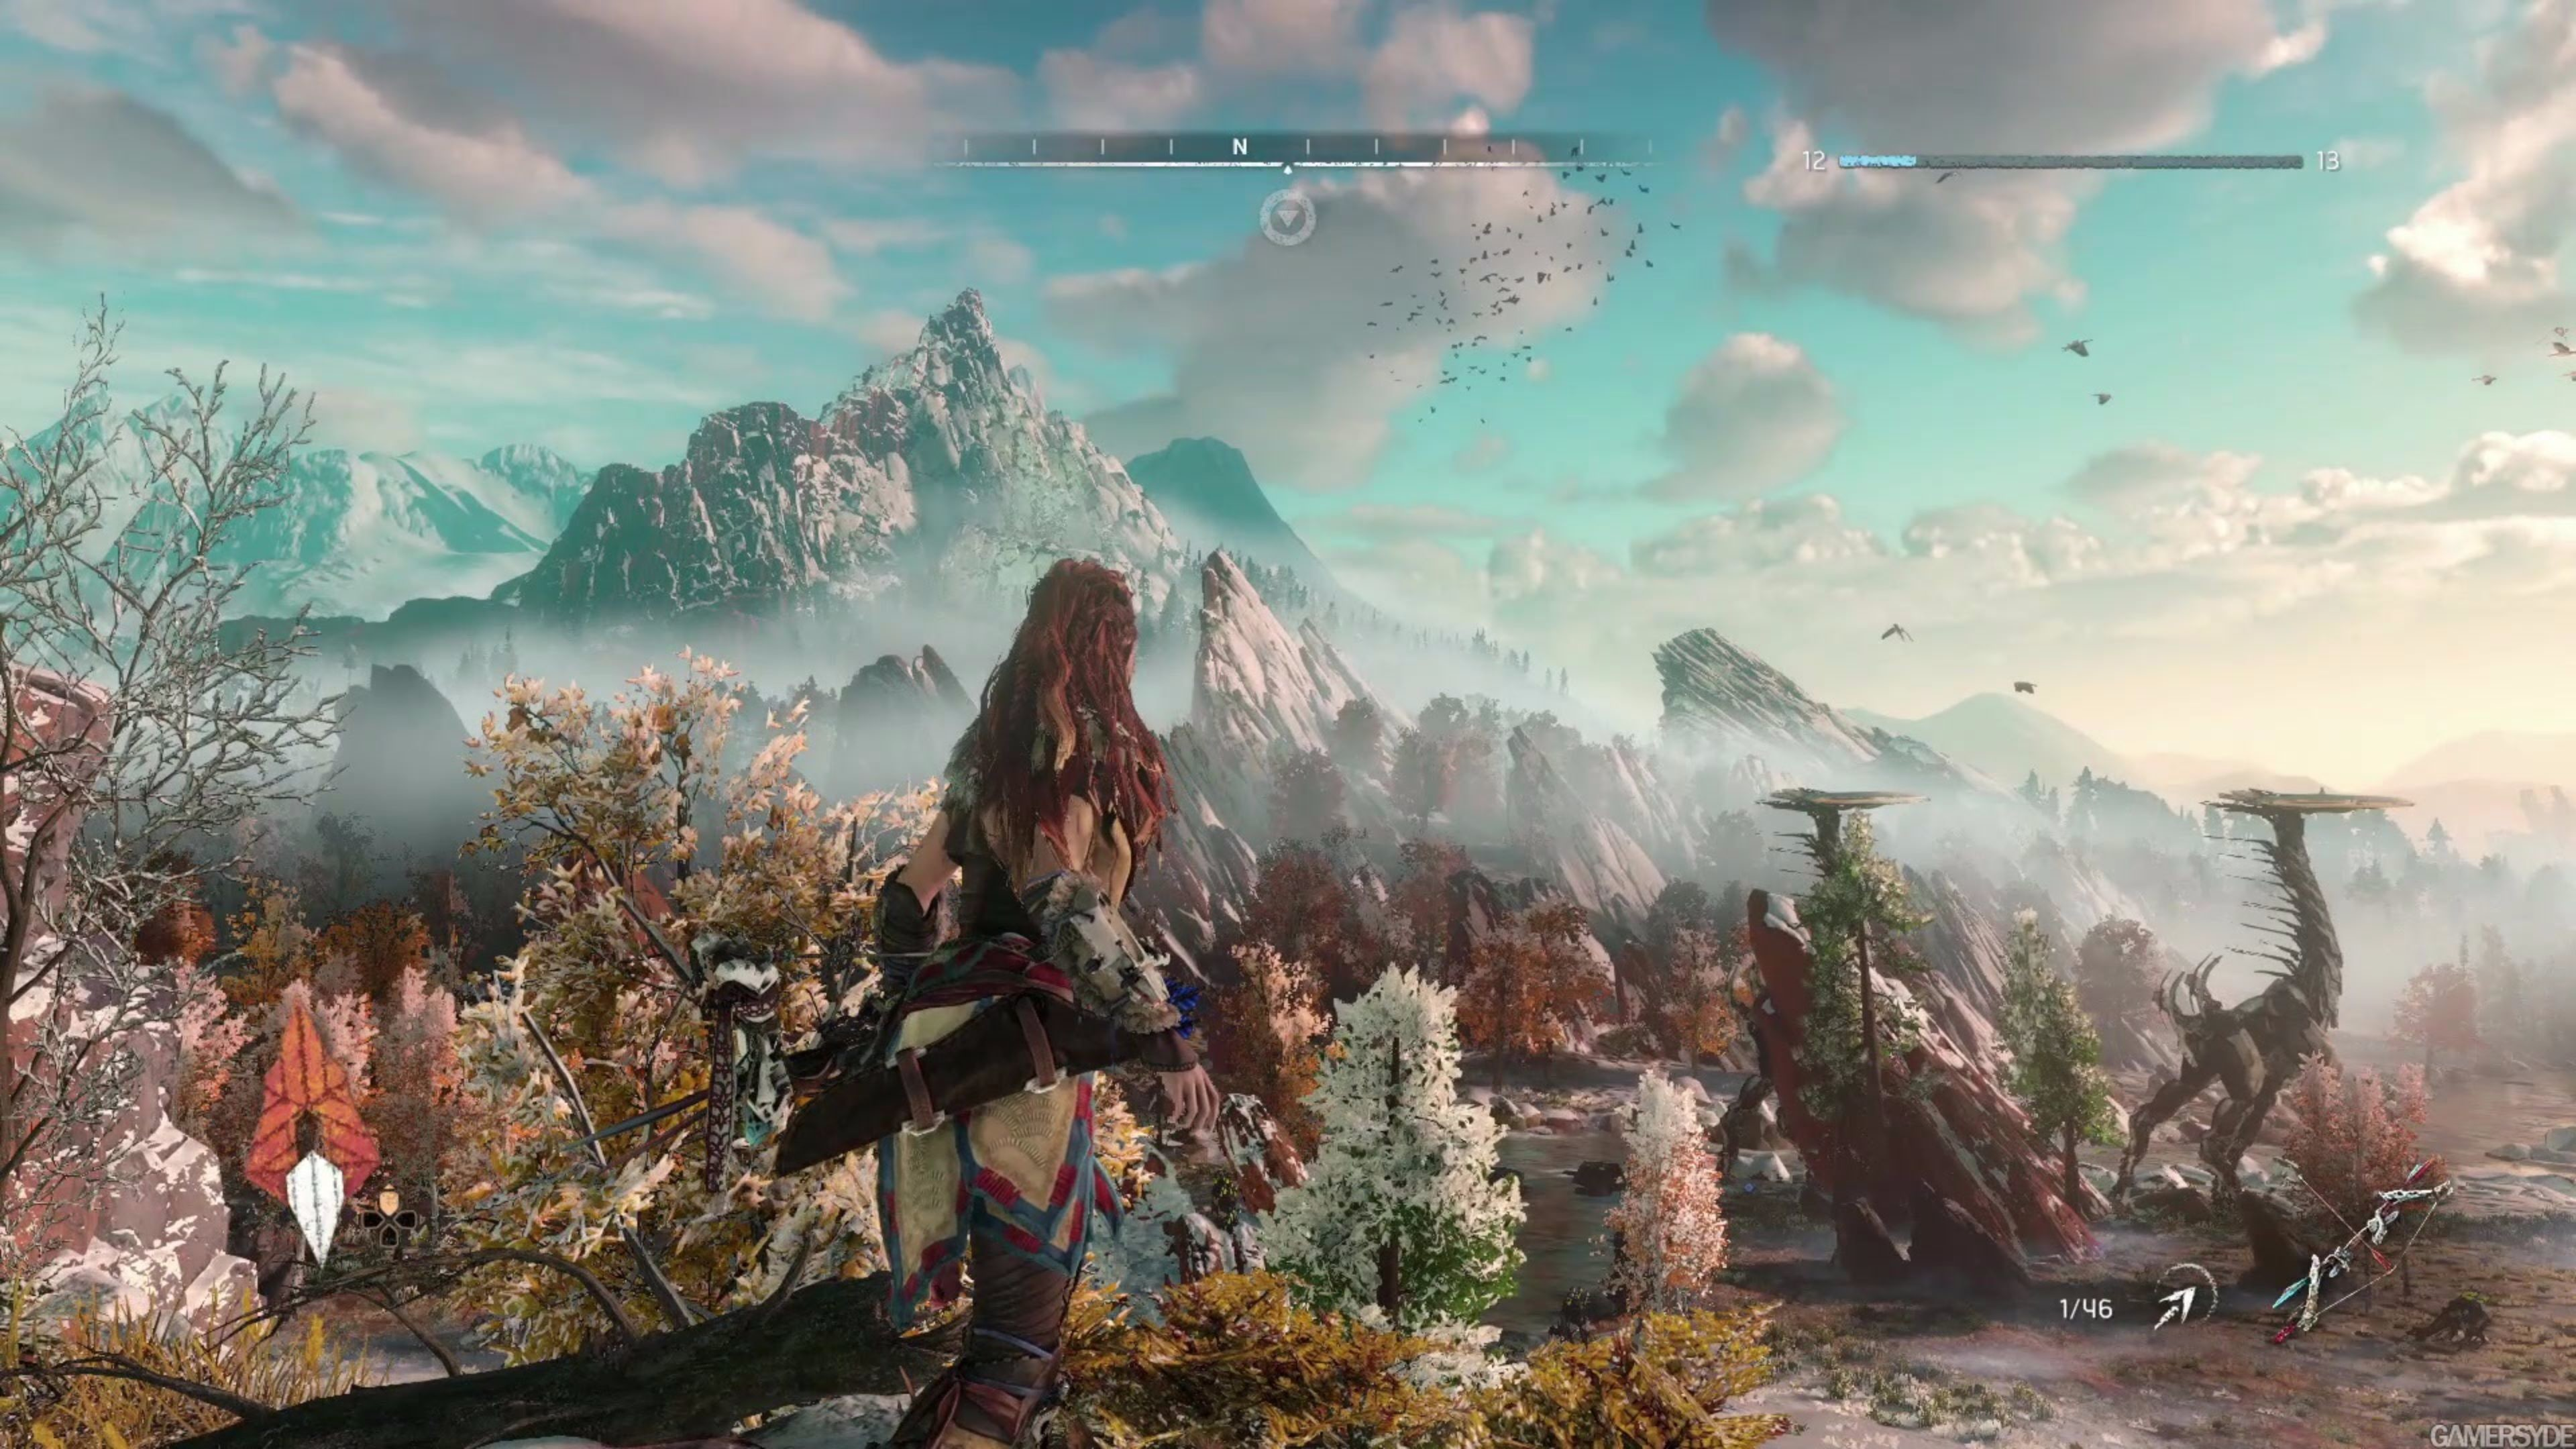
\includegraphics[width=\textwidth]{./Images/horizon-zero-dawn}
  \caption{Horizon Zero Dawn exquisite graphics.}
  \label{fig:horizon}
\end{figure}

\subsection{NPCs in games}

Most Triple-A video games make use of simple techniques to express \ac{NPC} behaviour.
Finite State Machines (FSM), hierarchical FSM and behaviors trees are the most commonly used techniques in nowadays industry \cite{yannakakis:gameairevisited}.
However simple, they can achieve believable and expressive behaviours in the hands of skilled game designers.
These techniques can express logic, basic planning and reactive behaviours.

Another advantage is that these techniques are deterministic, in other words, we can predict what can happen and then try to avoid problems.
Their major weakness, however, is their limited expressiveness, which can cause the realization of complex behaviors unmanageable.

In games like Assassin's Creed Unity \cite{games:assassinscreedunity} and Dragon Age Inquisition \cite{games:dragonageinquisition}, where there is a large number of \acp{NPC}, there is a tendency to make them reactive to the players instead of actively following their own goals.
In Dragon Age Inquisiton, many \acp{NPC} are present throughout the world doing absolutely nothing (check Figure \ref{fig:dragonage}).
Sometimes, when the player approaches, she can overhear a conversation that is taking place between \acp{NPC}, usually directly related to the player, but these are always simple one or two sentences conversations and the player cannot interact with the \ac{NPC} that is talking.

One can argue that, using current technology, it is impossible to make every single \ac{NPC} socially aware and able to interact with the player.
However, even if we only look at the \acp{NPC} with which we can interact, their behaviour is repetitive and lacks depth.

Other games, such as The Elder Scrolls V: Skyrim \cite{games:skyrim}, have \acp{NPC} with occupations which they carry out, during the day (the blacksmith will spend her day at the forge working), and houses where they return to, during the night (almost every character will go to his home to have a meal and sleep).
These simple behaviours highly contribute to the character's believability as it provides the sense of having wants and needs. However, they still lack social ability.

If, for example, the player breaks into the house of a random \ac{NPC}, wakes her up and has a talk with her, she will ignore the fact that you just woke her up in the middle of the night in her locked house and proceed to have a completely normal conversation with the player.
The weirder part still, is that the player will be branded as a criminal and may face the city's guards upon exiting the house.
This lack of social ability can easily break the player's suspension of disbelief.

To address this problem we can make use of research based agency models for \ac{NPC} control, as has been done in other works \cite{guimaraes:cif-ck-17}\cite{ferreira:merchant-model}.

\begin{figure}
  \centering
  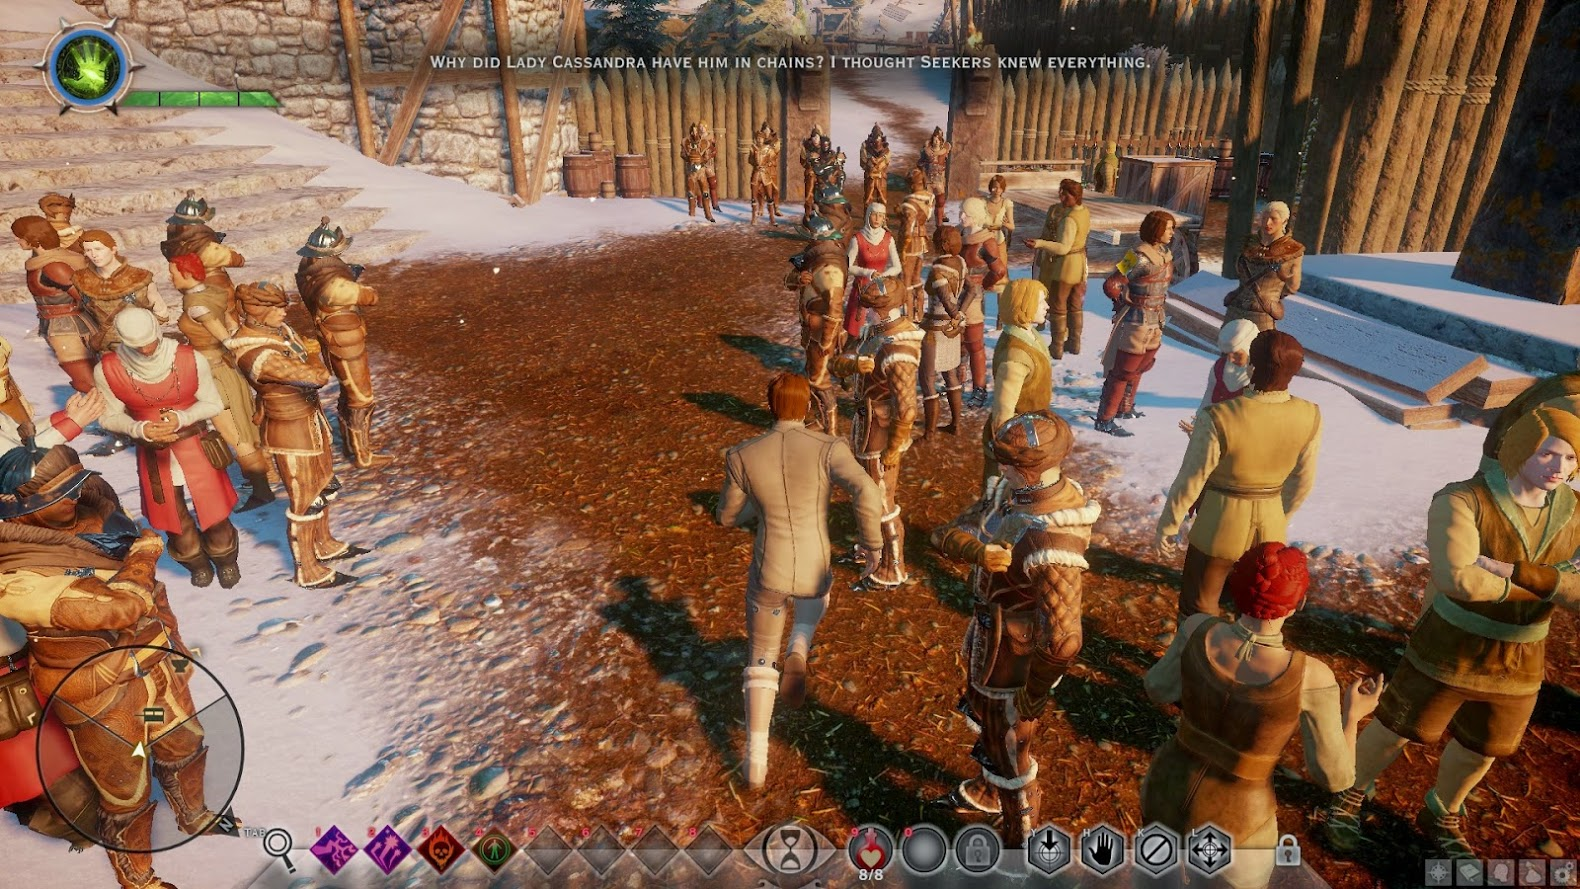
\includegraphics[width=\textwidth]{./Images/DragonAgeInquisition}
  \caption{Example of Dragon Age Inquisition's NPCs.}
  \label{fig:dragonage}
\end{figure}

\subsection{Socially empowered games}

\noindent There are, however, some examples of socially focused games that are worth to mention not only for their value as games but also for their successful use of research based agency models for \ac{NPC} control.

\subsubsection*{Blood and Laurels}
\label{subsection:bloodnlaurel}

Blood and Laurels (Figure \ref{fig:versu}) is a text-based interactive drama available in the App Store for the iPad\footnote{You can visit the game webpage at https://versu.com/2014/05/28/blood-laurels/.}.
One of the game's appeal is its high replayability due to the use of autonomous agents.
The same episode can be played several times with different results.
This is only made possible by making use of the Versu model \cite{evans:versu}, described in \ref{subsection:versu}.

\begin{figure}
  \centering
  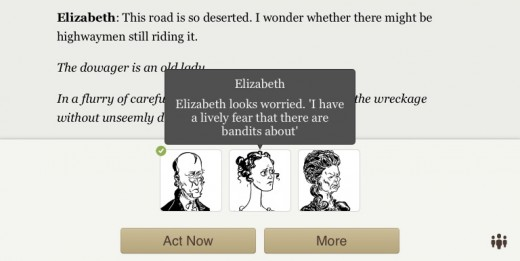
\includegraphics[width=0.7\textwidth]{./Images/versu}
  \caption{A screen shot of Blood and Laurels' game play.}
  \label{fig:versu}
\end{figure}

Blood and Laurels is set in ancient Rome and the player must weave through a web of conspiracies and politics.
The game's success and critics are proof that the use of socially aware \acp{NPC} can produce highly adaptable and interesting games.
The creators of Blood and Laurels are currently working on a second title called Bramble House which will also use Versu as the base for the autonomous characters (\acp{NPC}).

\subsubsection*{Prom Week}

\noindent Prom Week is a social simulation game about the interpersonal lives of a group of high school students in the  week leading up to their prom\cite{mccoy:prom-week}.
Gameplay in Prom Week involves solving level goals (such as making the class nerd, Zack, date a popular girl) within a limited number of turns by directing the characters to engage in social interactions.

What social games are available and how each changes the social state is managed by the game's \ac{AI} system, \ac{CiF}, described in \ref{subsection:cif}.
Enabled by the social physics of \ac{CiF}, each level's goal has innumerable solutions that maintain character believability.

\subsubsection*{Mismanor}

\noindent Mismanor is a social role-playing game where the player’s main form of interaction are actions that change the underlying social model \cite{sullivan:mismanor}.
It makes use of an adaptation of the \ac{CiF} architecture discussed in \ref{subsection:cif}.
In Mismanor, the player is guided through the dynamic story with quests that are chosen based on the actions the player has taken and their social standing with the character they are interacting with.
Quests have multiple entry and exit points, giving the player more flexibility with how they choose to fulfill the request, with different consequences based on the path they have taken.

\subsubsection*{Façade}

\begin{figure}
  \centering
  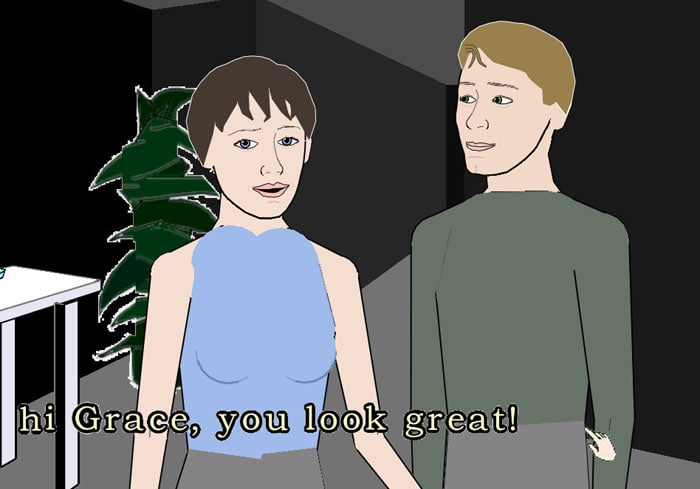
\includegraphics[width=0.7\textwidth]{./Images/facade-screenshot}
  \caption{The two NPCs of Façade greeting the player as she arrives at the dinner party.}
  \label{fig:facade}
\end{figure}

\noindent In Façade\cite{mateas:facade}, the player is given almost no direction or role to play.
The player can either play herself as the character or interpret the part of whomever she wishes.
The drama takes place in a small simulated virtual world, the apartment of the married couple Grace and Trip.
Façade was designed to deliver an experience that provides the player with 20 minutes of emotionally intense, undefined, dramatic action.
The player's actions have a significant influence on how the story develops and how the drama ends.

% \subsection{Research on Game AI}

% In Guimarães' work \cite{guimaraes:cif-ck}, \ac{NPC}s have social desires and complex behaviours and work towards changing the social state around them.
% The player can see them in action and decide whether or not he/she will interfere, introducing another kind of decision making in the game, one with immediate and visible consequences.

\section{Tools and Frameworks}

\noindent During this section we'll talk about some of the frameworks and tools currently available for the creation of agents.
We'll begin by presenting the well known Java framework \ac{JADE} and the \ac{FIPA} specification which \ac{JADE} is based upon.
Then, we'll talk of NetLogo and finally we'll present the PsychSim tool.

It is important to note that, to the best of our knowledge, there is, currently, no tool or framework that focuses in the development of \acp{NPC} for survival games.

\subsection{JADE}

\noindent \ac{JADE} is a software framework in compliance with the \ac{FIPA} specifications for interoperable intelligent multi-agent systems made in Java \cite{bellifemine:jade}.
It aims to simplify the development of agents while maintaining standard compliance through a comprehensive set of system services and agents.
\ac{JADE} complies with \ac{FIPA}'s specification \cite{obrien:FIPA} which defines the rules that allow a society of agents to operate, inter-operate, and be managed. This specification is further detailed bellow, in \ref{subsubsection:FIPA}.

While complying with the \ac{FIPA} specification, \ac{JADE} provides a set of abstractions that allow for the rapid development of agents, like the use of an abstraction model called Behaviour. 
Behaviours model the tasks that an agent is able to perform and each agent instantiates their behaviours according to their needs and desired capabilities.
The framework also includes some ready to use behaviours for the most common tasks in agent programming, such as sending and receiving messages and structuring complex tasks as aggregations of simpler ones.
The developer needs only to extend the Agent class and implement the agent-specific tasks through one or more Behaviour classes, instantiate them, and add the desired behaviours to the agent.

\subsubsection*{FIPA}
\label{subsubsection:FIPA}

\noindent The \ac{FIPA} specifications represent the first step towards an agent standard \cite{obrien:FIPA}.
The specification does not attempt to define the internal architecture of agents nor how they should be implemented, but they do specify the interfaces necessary to support interoperability between agent systems.
It identifies the roles of some key agents necessary for the management of the platform, and specifies the agent management content language, ontology, and agent communication.

Three key roles are identified as mandatory in an agent platform.
The Agent Management System is the agent that exerts supervisory control over access to and use of the  platform; it is responsible for authentication of resident agents and control of registrations.
The Agent Communication Channel is the agent that provides the path for basic contact between agents inside and outside the platform; it is the default communication method which offers a reliable, orderly and accurate message routine service.
The Directory Facilitator is the agent that provides a yellow page service to the agent platform.
Notice that no restriction is given to the actual technology used for the platform implementation: e-mail based platform, Java applications, web services... these could all be FIPA compliant implementations.

Agent communication is based on message exchange, where agents communicate by formulating and sending individual messages to each other.
The \ac{FIPA} \ac{ACL} specifies a standard message language by setting out the encoding, semantics and pragmatics of the messages.
The standard does not set out a specific mechanism for the internal transportation of messages.
Instead, since different agents might run on different platforms and use different networking technologies, \ac{FIPA} specifies that the messages  transported  between  platforms  should  be  encoded  in  a  textual  form.

Other  parts  of  the  \ac{FIPA}  standard  specifies  other  aspects,  in  particular  the  agent-software
integration, agent mobility and security, ontology service, and the Human-Agent Communication.

\subsection{NetLogo}

\noindent NetLogo (Figure \ref{fig:netlogo}) is a multi-agent programming language and modeling environment for simulating natural and social phenomena \cite{tisue:netlogo}.
Modelers can give instructions to hundreds or thousands of independent agents, called ``turtles".
These turtles can represent molecules, animals, people, bacteria, cars, robots, neutrons, magnets, planets, or whatever the modeler decides.
The turtles move across a grid of ``patches" which are also programmable agents.
All of the agents can interact with each other and perform multiple tasks concurrently.
This makes it possible to explore connections between micro-level behaviors of individuals and macro-level patterns that emerge from their interactions.

NetLogo comes with a Models Library, which contains several simulations.
This collection has more than 140 pre-built simulations that can be explored and modified.
These simulations address many areas in the natural and social sciences, including biology and medicine, physics and chemistry, mathematics and computer science, and economics and social psychology.

\begin{figure}
  \centering
  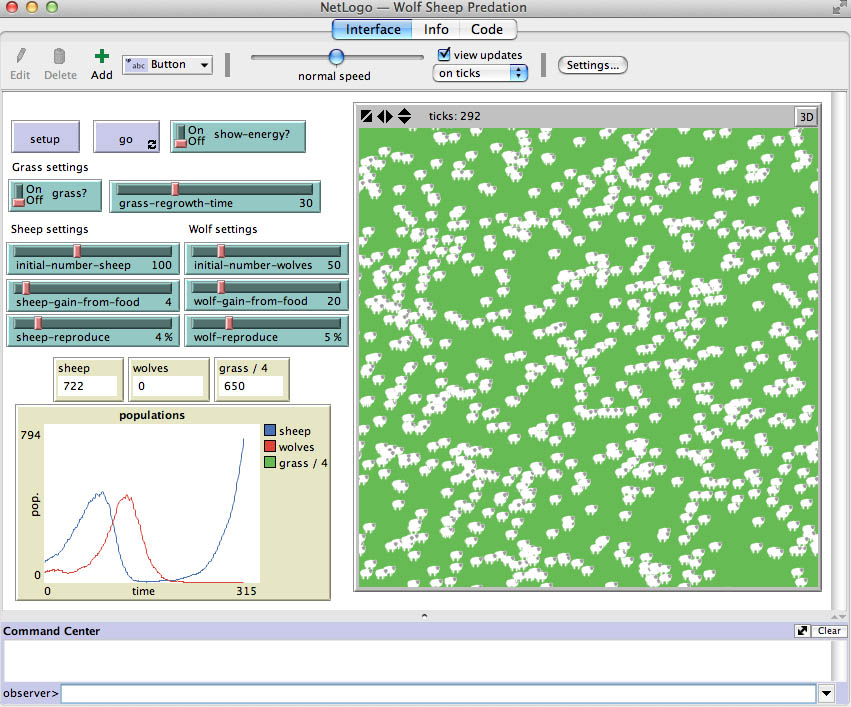
\includegraphics[width=0.7\textwidth]{./Images/netlogo5}
  \caption{NetLogo's interface.}
  \label{fig:netlogo}
\end{figure}

\subsection{PsychSim}
\label{subsection:psychsim}

\noindent PsychSim \cite{marsella:psychsim} is a social simulation tool developed to explore how individuals and groups interact and how can these interactions be influenced.
The work's foundation is the fact that social interactions are based on beliefs about other's minds, a \textit{theory of mind} \cite{whiten:theoryofmind}.
Psychsim allows developers to author and explore a social scenario of their creation through the selection of generic agents models and its further specialization, see Figure \ref{fig:psychsim}.
This tool allows developers to try and understand how a specific social group might react to certain situations.

\begin{figure}
  \centering
  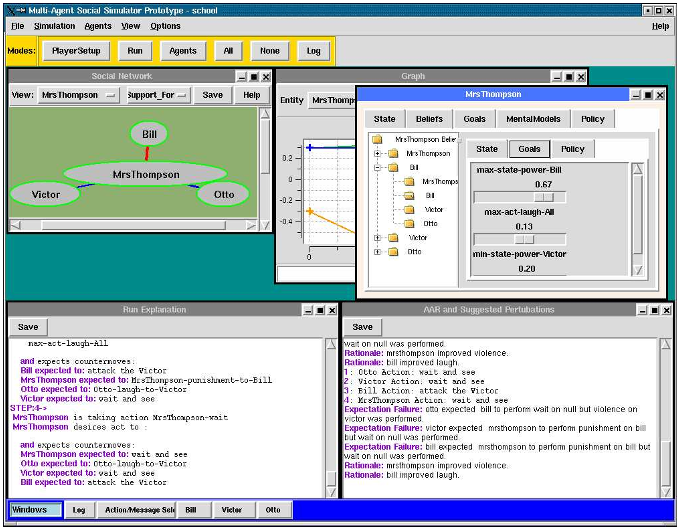
\includegraphics[width=0.7\textwidth]{./Images/psychsim}
  \caption{PsychSim tool for generating new scenarios and agents.}
  \label{fig:psychsim}
\end{figure}

PsychSim then simulates the behaviour for each entity, individual agent or group of agents, based on their preferences, relationships, private beliefs, and mental models about each other.

In the given example, the authors explore a bullying scenario in a school and try to answer several questions:
``\textit{How might a bully respond to admonishments, appeals to kindness or punishment? 
How might other groups react in turn? 
What are the predictions or unintended side effects?}".
The simulation tool then provides explanations of the results based on each entity's preferences and beliefs, allowing the authors to answer the previous questions.

PsychSim's agents are empowered with fully specified models of each other \cite{pynadath:modellingtheoryofmind}, a unique aspect of its design. Every agents maintains independent beliefs about the world, has its own goals, and it owns policies to achieve those goals. The model is composed by the state, actions, goals, beliefs, policies, messages, and mental models.

\begin{description}
\item \textbf{State} Each agent model includes a state with facts about the world, some of which may be hidden from the agent.
\item \textbf{Actions} Agents have a set of actions they can perform. Each action consists in an action type, a performer, and possibly an object of the action.
\item \textbf{Goals} These represent an agent's incentives for behaviours. In PsychSim, goals are reward functions that map the current state to a real value.
\item \textbf{Beliefs} The simulations agent have only a \textit{subjective} view of the world, where they form beliefs about what \textit{they} think is the state of the world. An agent's beliefs consists in models of all agents (including himself), representing their state, beliefs, goals, and policy of behaviour.
\item \textbf{Policies} Each agent's policy is a function that represents the process by which it selects an action or message based on its beliefs and goals.
\item \textbf{Messages} Messages are attempts by one agent to influence the beliefs of recipients and have five components: a source, recipients, a message subject, content, and overhearers.
\item \textbf{Mental Models} An agent's beliefs about another agent are realized as a fully specified agent model of the other agent, including goals, beliefs, and policies. Mental Models are predefined models which represent an agent's goals, beliefs, and policies.
\end{description}

\section{Social Architectures and Models}

\noindent In this section we take a look into existing models for agency.

\subsection{Comme il Faut and Ensemble}
\label{subsection:cif}
\noindent \ac{CiF} is an \ac{AI} system that enables authors to create interactive stories by specifying, not the complete narrative and all its ramifications but, high-level rules governing expected character behaviour given social situations \cite{mccoy:cif-social-story-worlds}.
In \ac{CiF}, characters use many attributes of the current social state, including the story of prior interactions, to decide how to engage in social exchanges with other characters.
This architecture provides a rich social environment for characters to interact allowing the creation of dynamic and interactive stories.

%\ac{CiF} does not store world information in a series of events, like many \ac{AI} techniques do (e.g. Behaviour Trees and Hierarchical Task Networks).
Social exchanges are the primary structure of representing knowledge in \ac{CiF} \cite{mccoy:cif-authoring}.
They consist in social interactions between characters that modify the social state of the participants.
By using social exchanges and additional encoded social context, \ac{CiF} lowers the authoring burden needed to create the social aspects of an interactive story by allowing the author to specify the rules and general patterns of how social interaction should take place.

Characters' behaviour is chosen based on rules in a large rule database that depict normal social behaviour in a particular story world.
These rules, in conjunction with the logic of a social world, a set of characters, and a series of scenario goals allows \ac{CiF} to determine the desired action for each character.

More recently, a new version of \ac{CiF} as been published and renamed to Ensemble.
Ensemble aims to empower \acp{NPC} with deeper interactivity and believability by modeling social states and behaviours for game characters \cite{treanor:ensemble}.
This extension presents a model of playable social dialogue called social practices.
Social practices increase the playability of character interactions and add interactivity at each stage of dialogue.

\subsection{Versu}
\label{subsection:versu}

\noindent Versu model is based on Exclusion Logic \cite{evans:exclusion-logic}, a new deontic logic, and rests upon two kinds of objects: agents and social practices.
To better make use of exclusion logic, the creators of Versu have also developed Praxis, a \ac{DSL} used in the modeling of the social practices .

Social practices describe a recurring social situation that may exist only for a short time (e.g. a conversation, a game, a meal) or can last much longer (e.g. a family, the moral community).
These practices coordinate agents via the \textit{roles} they are playing and their main function is to describe the actions the agents can do in each situation.

Social practices provide the agent with a set of suggested actions, but it is up to the agent to decide which action to perform, using utility-based reactive action selection (the utility is calculated in accordance with the agents beliefs, desires, personality quirks, and backstory).

Multiple practices can exist concurrently, for example, in a dinner party, there will be multiple practices operating at once:

\begin{itemize}
\item eating and drinking.
\item the conversation about politics
\item the rising flirtation between Frank and Lucy
\item responding to the fact that Mr. Quinn has spilled the soup.
\end{itemize}

Performing an action can result in any sentence being added to the world database.
The results of adding new sentences can be that relationships are updated, new beliefs or desires are formed, old practices are deleted or new practices are spawned.
Agents and social practices are scripts authored using the \ac{DSL} Praxis.

\subsection{FAtiMA}
\label{subsection:fatima}

\noindent \ac{FAtiMA} is an agent architecture with planning capabilities designed to use emotions and personality to influence the agent's behaviour \cite{dias:fatima-modular}.
The acronym stands for Fearnot AffecTIve Mind Architecture as it was developed to endow the characters in the serious game \textit{FearNot!} \cite{aylett:fearnot} with social intelligence.
It has been used successfully in different social scenarios (\cite{paiva:learning-by-feeling},\cite{rodrigues:i-can-feel-to}, \cite{aylett:intercultural-empathy}, and \cite{correia:sueca}) and it is based on appraisal theory \footnote{The theory that emotions are elicited by evaluations (appraisals) of events and situations \cite{roseman:appraisal}.}.

\ac{FAtiMA} has a modular architecture where functionalities and processes are divided into modular independent assets.
This enables developers to use a lighter and simpler version of \ac{FAtiMA} by adding the required assets, according to their necessities.
Therefore, behaviour and functionality are added by including assets in an agent's definition.
These assets will then implement the desired behaviours and functionalities.

\ac{FAtiMA} comes with a set of predefined assets that can be used to define agents and their interactions\footnote{The toolkit is available at https://github.com/GAIPS-INESC-ID/FAtiMA-Toolkit.}.
Additionally, the developer can create its own assets that extend the toolkit's capabilities.
The available assets are:

\begin{figure}
  \centering
  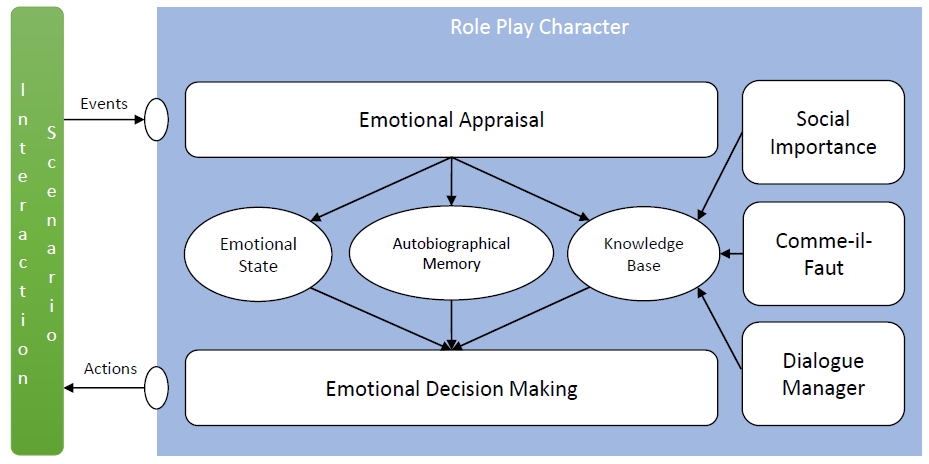
\includegraphics[width=\textwidth]{./Images/rpc}
  \caption{The Role Play Character Asset aggregating all other assets to make an autonomous agent.}
  \label{fig:rpc}
\end{figure}

\begin{description}
\item [Role Play Character Asset] \hfill

The \ac{RPC} Asset is an aggregation asset responsible for managing all the other assets that compose an agent.
It is also responsible for maintaining the agent's Emotional State and the agent's memory, which is divided in two components: a Knowledge Base and an Autobiographic Memory.

The Emotional State stores the current emotional state of the agent, defined by the Emotional Appraisal Asset, the Knowledge base stores the agent's beliefs, and the Autobiographic Memory stores the agent's recollections of past events and the emotions associated with such events.

Events are divided into three categories: Action-Start, Action-End, and Property-Change. The first two are self-explanatory and the third represents updates to the \ac{RPC}'s Knowledge Base.
Therefore, in order to update the Knowledge Base, the \ac{RPC} must perceive the appropriate events.

For consistency sake, both beliefs and events are described by \ac{WFN}.
These can be symbols (e.g. ``\texttt{Walter}" or ``\texttt{cutgrass}"), variables (e.g. ``\texttt{[x]}" or ``\texttt{[target]}"), and composed names (e.g. ``\texttt{IsBusy(Walter)}" or ``\texttt{Likes(Walter, [target])}").

\item [Emotional Appraisal Asset] \hfill

This asset appraises each event according to the OCC Theory of Emotions \cite{ortony:occ}.
Developer defined appraisal rules, determine how an agent evaluates certain events, determining the agent's Emotional State (which is kept by the \ac{RPC}).

For example, an agent, Mary, who likes John, might perceive the event of John flirting with her in a positive way, whilst another agent, Kate, who dislikes John, might perceive such flirtation negatively.

\item [Emotional Decision Making Asset] \hfill

The Emotional Decision Making Asset provides \acp{RPC} with decision making capabilities based on rules with logical conditions.
Allowing the agent to make multiple decisions at the same time, this asset makes use of the Knowledge Base and the Emotional State to decide which actions it decides to do.

The possibility of making multiple decisions at the same time is particularly interesting when considering behaviour related decisions and non-behaviour related decisions (dialogue actions and/or emotional responses).
\ac{FAtiMA} Toolkit handles this by making use of what it calls layers of decisions.
When the decision process is triggered, if a layer is provided, only actions for that layer are considered.

Additionally, this asset adds Dynamic Properties that can be used as conditions to actions.
Dynamic Properties provide a facility for developers to implement additional processing capabilities for the decision of certain actions.
For example, the developer could implement a \textit{Gaze} Dynamic property that would connect to an external eye tracking device, in order to make the agent act in accordance to the user's gaze.

\item [Integrated Authoring Tool Asset] \hfill

This asset adds a Dialogue Manager that combines an hybrid solution between dialogue trees (a popular solution among game developers) and state machines to construct dialogues for agents.
The Dialogue Manager keeps the current state of dialogue, giving an agent (or player) every available option to choose from.
This is achieved through the implementation of the \textit{ValidDialogue} Dynamic Property, that will advance through the Dialogue Manager.

\item [Social Importance Asset] \hfill

The Social Importance Asset implements the \textit{SI} Dynamic Property, which represents the social relationship among two social entities A and B.
This representation, based on the status-power theory \cite{kemper:status-power}, gives information about how willing an agent is of complying with another agent's wishes.

Note that the social importance relationship is not equivalent, meaning that the social importance that agent A gives to agent B might not the same as the social importance that agent B gives to agent A.
The social importance values are maintained by a set of developer defined attribution rules that are evaluated after an event is perceived.

\item [Comme il Faut Asset] \hfill

Based in the work previously described in \ref{subsection:cif}, this asset allows developers to define Social Exchanges which, unlike single dialogue acts, are composed by sequential steps: initiate, answer, and finalize.
These steps represent an interaction between two agents.

Each of the steps share the activation conditions of the Social Exchange, and can have different styles (positive, neutral, and negative) that are calculated by the \textit{Volition} Dynamic Property, introduced by this asset.

\item [World Model Asset] \hfill

The World Model Asset gives developers a way to test the created agent in a simulated world where the consequences of each action is defined by the developer.
This asset is especially useful to test particular aspects of an agent.

By using the \ac{FAtiMA} Authoring Tools, the developer can specify the complete current state of an agent and run it in this controlled environment.
It also gives the developer a way to simulate the world the agent is in. which is particularly useful when we consider planning agents.

\end{description}

It is important to note that the \ac{CiF} Asset can be used to complement the Social Importance Asset by giving an agent knowledge about social practices.
For example, while a boyfriend and father might have equally high social importance values, flirting is not an appropriate social practice when the target is the agent's father.
By defining flirting as a social exchange, the developer can define an additional condition to only activate this social exchange if the agent is attracted to the target.


% \ac{FAtiMA}\footnote{The toolkit is available at https://github.com/GAIPS-INESC-ID/FAtiMA-Toolkit.} is an agent architecture with planning capabilities designed to use emotions and personality to influence the agent's behaviour \cite{dias:fatima-modular}.
% It has been used in different scenarios (\cite{paiva:learning-by-feeling},\cite{rodrigues:i-can-feel-to}, \cite{aylett:intercultural-empathy}, and \cite{correia:sueca}) and it is based on appraisal theory \footnote{The theory that emotions are elicited by evaluations (appraisals) of events and situations \cite{roseman:appraisal}.}.

% \ac{FAtiMA} has a modular architecture where functionalities and processes are divided into modular independent components.
% This enables users to use a lighter and simpler version of \ac{FAtiMA} by adding the required components to the \ac{FAtiMA} Core.

% However, \ac{FAtiMA} Core does not commit itself with the particular methods used.
% In fact a FAtiMA agent that only has a Core will not do anything.
% Behaviour is added by adding components that implement the mentioned functionality.

% Currently, \ac{FAtiMA} counts several already defined modules which the user can use out of the box (e.g. Cultural Behaviour \cite{mascarenhas:cultural-behaviour} and Drives \cite{lim:affective-npcs}, among others) but it can also write new modules to add different functionality to the model.
% The architecture of \ac{FAtiMA} Core can be seen in Fig. \ref{fig:fatima-core}

% \begin{figure}
%   \centering
%     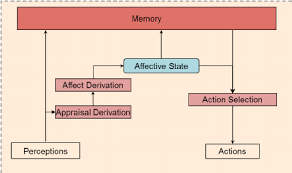
\includegraphics[width=.8\textwidth]{./Images/fatima-core}
%   \caption{FAtiMA Core's architecture.}
%   \label{fig:fatima-core}
% \end{figure}

% An agent is able to receive perceptions from the environment (events) which are used to update the agent's memory (or internal state) and to trigger the appraisal process.
% The result of the appraisal process is stored in the affective state, and later used to influence the action selection processes which will make the agent act upon the environment.
% Appraisal Derivation is responsible for evaluating the relevance of the event to the agent and determines a set of appraisal variables and affect derivation takes these variables as input to generate the resulting affective states (emotions or mood).

% As noted before, an agent using the \ac{FAtiMA} Core on its own will do nothing.
% Agency is achieved by adding several components (or modules) to the Core.
% In the scenario described in \cite{mascarenhas:cultural-behaviour}, the author used the following components:

% \begin{itemize}
% \item \textbf{Reactive Component}: uses a set of emotional reaction rules to determine values of some appraisal variables.
% \item \textbf{Deliberative Component}: handles goal-based behaviour and adds planning capabilities to the agent. It also uses the state of plans in memory to generate appraisal variables.
% \item \textbf{OCCAffectDerivation Component}: generates emotions from the appraisal variables according to the OCC Theory of Emotions \cite{ortony:occ}.
% \item \textbf{Motivational Component}: models needs and goals for the agent that will influence the utility of a given goal.
% \item \textbf{Theory of Mind Component}: creates a model of the internal states of other agents.
% \item \textbf{Cultural Component}: implements cultural-dependent behaviour of agents through the use of rituals, symbols, and cultural dimensions, and determine the impact actions have on the motivational states of the agents.
% \end{itemize}

\section{Closing Remarks}

\noindent The game industry is currently using outdated techniques to add behaviour to the characters that populate their games.
Skilled game designers can still create interesting behaviours with the used techniques, but the need for social context and active goal pursuit requires more advanced techniques.

To build a platform that will enable developers to create collaborative and believable \acp{NPC} for survival games, we've, first of all, looked into frameworks and tools that focus on agent creation.

\ac{JADE} provides a great platform for the development of agents.
However, \ac{JADE}'s main field of applicability is that of software engineering.
Its main purpose is the development of negotiating agents that conform to the \ac{FIPA} specification, having no concern whatsoever for interactions with humans, to such an extent that, although it is specified in \ac{FIPA}, \ac{JADE} is an agent-only platform with no support for Human-Agent Communication. 

NetLogo is a great example of testability, which is one of our main focus.
The ability to run fine tuned scenarios with different behaviours easily is a key point of its design and of utmost importance for our work, and that we will strongly value while developing our work.
Despite that, it does not provide a model for agency which is one of the crucial points of this work.

The final tool we've looked into is PsychSim.
As a social agent architecture, PsychSim presents a well-defined model capable of fully simulating social behaviour, is based on sound theories from psychology, and takes into account other agents in its cognitive process.
But, it lacks the possibility to have agents interacting with humans.
Additionally, as the agent's behaviour is based only in policies which guide it's immediate behaviour, each agent will follow the scenario devised by the developer without deviation.

We've then moved into exploring some of the currently used agency models.
The three systems we described were \ac{CiF}, Versu, and \ac{FAtiMA}.

Despite the successful implementation of \ac{CiF} in the game Prom Week \cite{mccoy:prom-week}, the game developers still need to specify every rule for every possible social interaction between \acp{NPC}.
Prom Week contains over forty nine hundred unique influence rules, around sixty social exchanges with over twenty rules that contribute to the characters' desires and responses, a cast of eighteen characters, and a combined total of over forty thousand predicates.
This represents an authoring burden that we want to avoid when developing our \acp{NPC}.
Even its successor, Ensemble, which lowers the authoring burden by adding social practices, has been recognized, by the authors, to possess limitations: a social practice must be taken to completion before another practice can be initiated, which does not reflect real social interaction.

Versu's logic powered approach is a differentiating aspect from the other models, however it does imposes some limitations.
One example is how the agents beliefs are expressed.
The system cannot represent universal and existential quantifiers (e.g. ``everyone has become insane" and ``the murderer is one of the guests", respectively) or beliefs about others' beliefs (e.g. ``Mr Quinn believes that Lucy believes that Mrs Quinn is the murderer").

Finally, and although \ac{FAtiMA}, by itself, is not a determined model for agency, it provides a set of ready to use assets, that allow developers to use whatever they need to achieve their goals.
The inclusion of emotional appraisal, theory of the mind models, and its planning capabilities make \ac{FAtiMA} the best candidate to be used.
This, allied with the fact that it has been successfully used in several social scenarios with human interaction (\cite{paiva:learning-by-feeling} \cite{rodrigues:i-can-feel-to} \cite{aylett:intercultural-empathy} \cite{correia:sueca}), the ability to extended the existing assets, and the ability to incorporate planning into its decision making process, make it the best choice for our work.


% If Printing on DOUBLE SIDED pages, the second page should be white.
% Otherwise, comment the following command:
\cleardoublepage
%
%Chapter 3
% #############################################################################
% This is Chapter 3
% !TEX root = ../main.tex
% #############################################################################
% Change the Name of the Chapter i the following line
\fancychapter{Case Study: Don't Starve Together}
\cleardoublepage
% The following line allows to ref this chapter
\label{chapter:case-study-dst}

\noindent Don't Starve Together is a multiplayer wilderness survival game developed by Klei Entertainment, where the players must survive as long as they can.
The players must face the harshnesses of a procedurally generated world that is actively trying to kill them, either by cooperating or competing with each other.
Each game can last an indefinite amount of time which is only determined by the players' ability to survive: the better you play the game, the longer you can last.

Released on April 21st of 2016, \ac{DST} is the standalone multiplayer expansion of the uncompromising wilderness survival game Don't Starve, also released by Klei on April 23rd of 2013 (check Fig. \ref{fig:don't-starve-together-poster}).
Both titles are available in several platforms ranging from PC's to consoles and even mobile devices.
By the end of 2013 the original title (Don't Starve) sold over one million copies and, currently, there are almost 3.5 million owners of the game only on Steam.
\ac{DST} counts with over 7 million owners on Steam and has a daily peak of concurrent players of about 8 thousand, reaching as high as 12 thousand concurrent players.

\begin{figure}
  \centering
  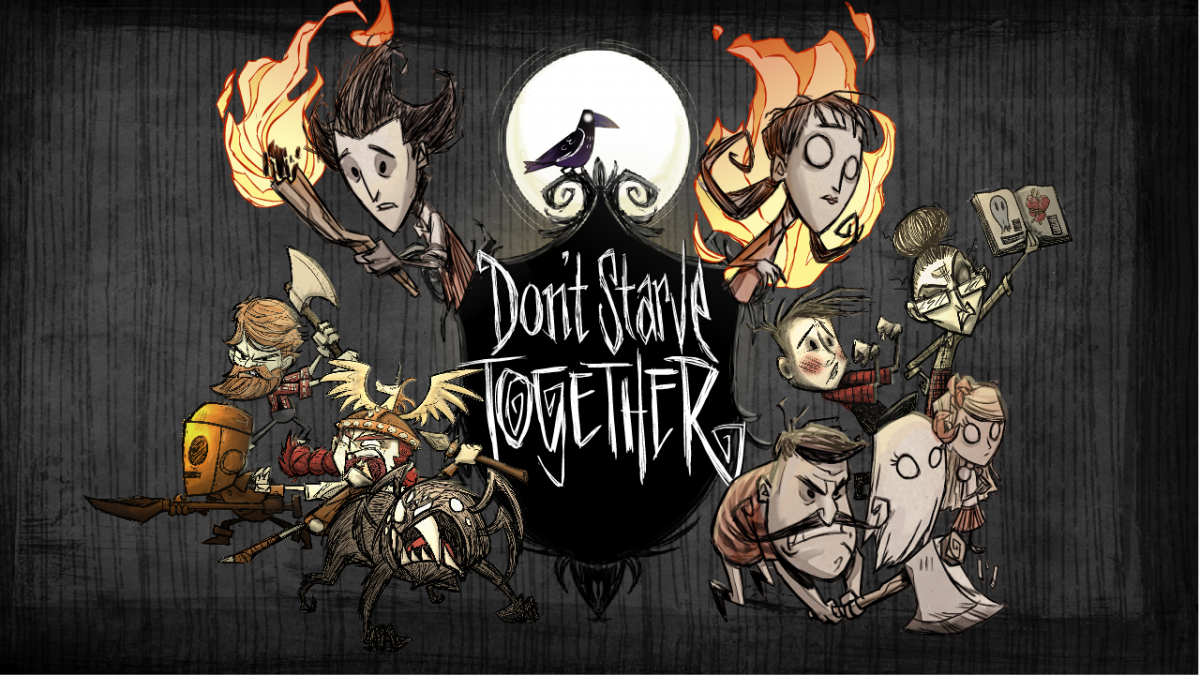
\includegraphics[width=\textwidth]{./Images/dont-starve-together-poster}
  \caption{Don't Starve Together poster with all original characters.}
  \label{fig:don't-starve-together-poster}
\end{figure}

The game counts with a developer maintained forum where there is an active participation by Klei Entertainment staff, which help in problem solving for community developed mods, bug fixing the game, and sharing development notes on the game.
Currently, over five thousand mods are available for the game on the Steam Workshop.

As we've previously discussed, survival games offer players different challenges that must be overcome by the character in order to survive.
Some do it by providing mechanics for hunger and thirst while others provide horrific scenarios like zombie infested worlds.

\ac{DST} borrows ideas from both sides.
The game presents mechanics for hunger, health, temperature, wetness, day and night cycles, seasons, and sanity.
It also provides players with a monster infested world that try to kill the player's character.
The addition of multiplayer brings the possibility for social interaction among players, which contributes positively for the gameplay experience.

Moreover, the sanity mechanic itself is a differentiating factor from other games in the genre.
By providing a measurement of the characters' mental health, the game makes the characters more human and relatable.
A normal human being under such harsh environments would suffer physically but also mentally, and the sanity mechanic depicts just that.

For these reasons, the lack of \ac{AI} controlled \acp{NPC} with believable behaviour, the ability to control and personalize the generated game world, and the possibility of introducing modifications into the game, we've decided to use this game as the target of our project.

For the remainder of this chapter we will present a thorough break down of the game.
We'll explain what the game consists in and move on to describing the game's world.
Then, a general gameplay experience is briefly described before ending the chapter with a summarization of the game mechanics.

\section{The Game}

\noindent Before playing \ac{DST}, the player must first generate a game world to play in.
The generation process will create a new world in accordance to a set of configurations.
The configurations allows her to personalize every aspect of the game world, including the world size, the abundance of resources, the existence and frequency of monster appearances, and many more options.

The player will then choose a character from a list of available characters.
Different characters have different characteristics and may be affected by the world in different ways (for example, WX-78 can eat spoiled food without penalties) and can even possess special items (such as Woodie's axe, \textit{Lucy the Axe}).
Upon entering the world, the player has nothing in its inventory (except for character specific items) and thus needs to start collecting resources in order to survive.

During the game, the player must pay attention to the three characteristics of her character: Hunger, Sanity, and Health.
The player dies (in \ac{DST} the player actually becomes a ghost that can be revived by other players or by finding a Touch Stone) once his Health reaches zero.
Both Hunger and Sanity can cause the player to loose Health (Sanity doesn't directly cause the player to loose Health, but the player will be attacked by creatures that appear due to the character's paranoia).

So, it is important for the player to keep Hunger, Sanity, and Health in check in order to survive.
The player will also need to take attention to the character's Wetness which is caused by rains.
Wetness will cause the items to loose efficiency and by using wet items the character will lose Sanity over time.
The player must also be aware of the temperature of his character as it can cause damage.
Both extreme hot and extreme cold will cause the player to continuously loose Health.

Taking care of the character's Hunger, Sanity, and Health is the player's main concern during gameplay.
She will accomplish this by collecting resources, crafting new items, cooking food, among other things (we will explore the player's possible actions in full detail further on).

\section{The World}

\begin{figure}
  \centering
  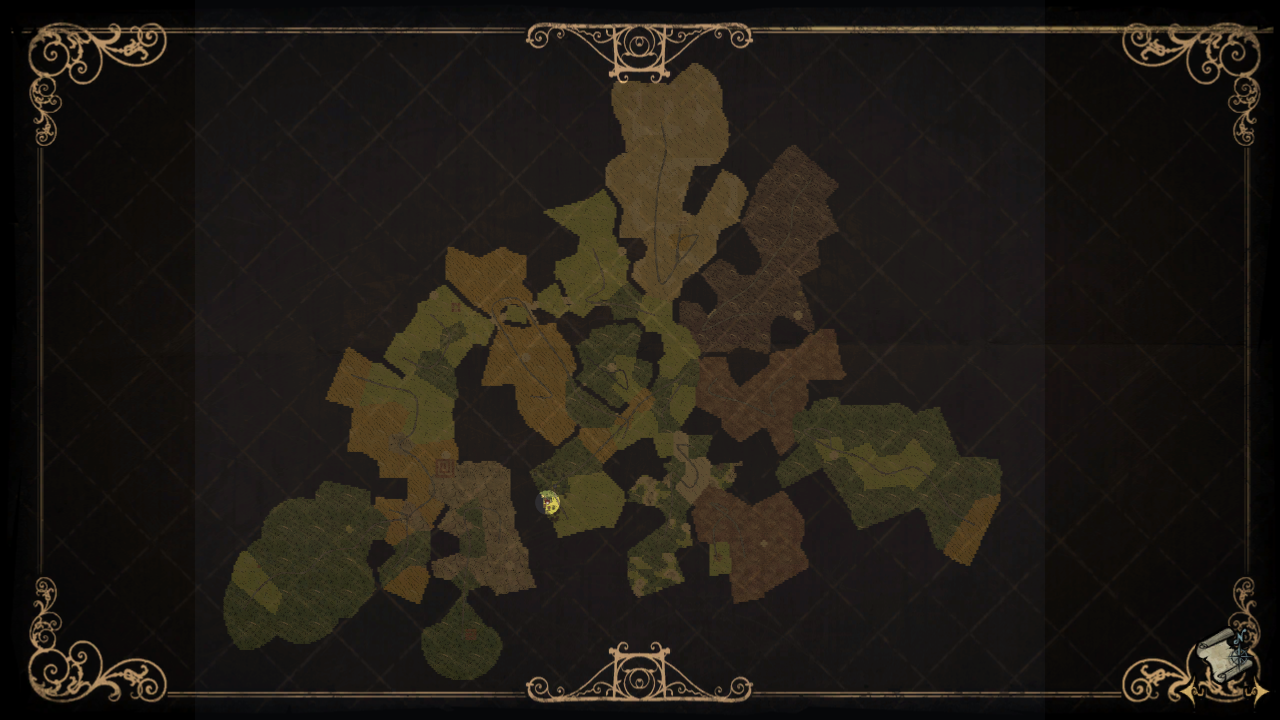
\includegraphics[width=\textwidth]{./Images/world-map}
  \caption{Example of a generated map of \ac{DST}.}
  \label{fig:world-map}
\end{figure}

\noindent As mentioned earlier, the world is procedurally generated for each game and has several different biomes that provide different kinds of resources but also dangers for the player. 
We'll present and describe these biomes later on.

The world is surrounded by water and is, in many cases, composed by several peninsulas which can be composed by one or several biomes, as can be seen in Fig. \ref{fig:world-map}.
It's also common to see the formation of lakes inside the main portion of land.

During gameplay, time will pass not only in a night and day cycle but also across seasons.
The game has four seasons (Autumn, Winter, Summer, and Spring) that present different challenges during the course of the game.
In Winter, the temperature descends a lot, while in Summer, the temperature rises, causing the player to take damage over time due to extreme temperatures.
In Spring, the commonly occurring rains will increase the character's Wetness, which will have the effects already described.
Autumn is by far the friendlier season, with mild temperatures and occasional rains, making it the perfect candidate for the starting season.

Seasons bring yet another challenge for players: giants (see Fig. \ref{fig:dst-deerclops}).
During each season, a giant (for each season there is the corresponding giant) will spawn in the vicinity of the player and will attack him.
The player can either choose to engage in a fight with the giant or try and lure him away until the giant looses interest.

A normal world will also have caves that the players can descend to, but we will not discuss them here since we won't consider them for our work.

\begin{figure}
  \centering
  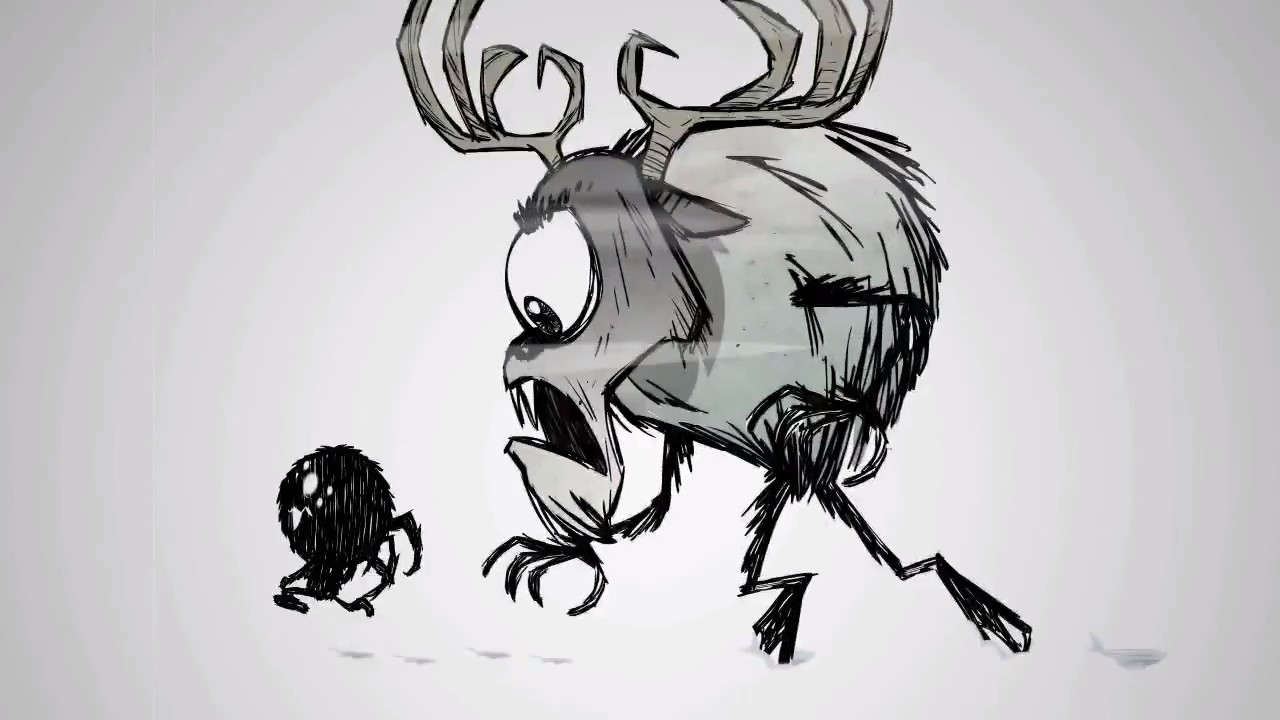
\includegraphics[width=\textwidth]{./Images/dst-deerclops}
  \caption{Deerclops, the Winter giant, chasing after Webber.}
  \label{fig:dst-deerclops}
\end{figure}

Moving on to the specifics of each biome, we'll now explore a list of all the available biomes on \ac{DST} and a brief description for each of them:

\begin{itemize}
\item \textbf{Chess} this biome has an abundance of marble (a very rare material in the game), however it is protected by aggressive mobs;
\item \textbf{Deciduous Forest} being a forest, this biome is a great source of wood but also fireflies and mushrooms;
\item \textbf{Desert} can be a good source of grass and twigs (two of the most important resources on the game) but can also be very dangerous due to the Hound mob spawn points;
\item \textbf{Forest} a very good source of wood but can also contain spiders;
\item \textbf{Grassland} one of the safest biomes where the player can find a good variety of resources;
\item \textbf{Graveyard} can contain many gold nuggets and can be hazardous free.
By digging up graves the player can collect loot but there is a chance that a Ghost may spawn and attack the player.
\item \textbf{Marsh} commonly known as Swamp, is the harshest biome in the game, everything here will try and kill the player;
\item \textbf{Mosaic} this biome typically appears only once per map, and is a mix of all other biomes with not so great resources;
\item \textbf{Savanna} the abundance of grass and mobs (passive mobs like Rabbits, Birds, and Beefaloes) make this biome the best for the player to settle.
Although it can also become a dangerous place during the Beefaloes mating season where they become aggressive;
\item \textbf{Rockyland} a barren biome that contains a lot of boulders but almost nothing else. It’s a common place for Tallbirds, an aggressive mob.
\end{itemize}

%For a complete listing of all the resources and where to find them, see Appendix B.

The knowledge of each of these biomes will differentiate good players from expert players, as it can strongly influence their success.
Players must know where to for look what they need, where to settle, places to avoid, among others.

For the remainder of this section, we'll explore the environment of \ac{DST} which we just described in a more formal way.

According to Russel and Norvig's classification of environments \cite{russell&norvig:aima}, \ac{DST} is a partially observable, multiagent, stochastic, episodic, dynamic, continuous, and known environment.

\begin{description}
	\item \textbf{Partially observable} In \ac{DST} the environment is actually fully observable through the scripts it natively provides to the modders and every entity is directly accessible to the agent. Despite this, we've decided to limit the observability of the environment to keep the agent in the same level of knowledge with the player, therefore, it will only have access to the same area as seen by the player in the screen.
	\item \textbf{Multiagent} The world may contain several players, and is therefore a multiagent environment.
	\item \textbf{Stochastic} During the game, spontaneous rains can occur, meteors can fall from the skies, and even lightning strikes can set the players crops ablaze. 
	This all happens randomly and the agent will need to act accordingly in order to survive.
	\item \textbf{Episodic} Although the world is in a continuous flow, we can consider it an episodic environment. 
	Due to the continuous passage of time, day after day and season after season, the player will have to overcome recurring problems.
    Every night the player will have to deal with darkness (which can kill the player) and every season similar challenges (Winter always presents the same challenges).
	\item \textbf{Dynamic} During the deliberation process of the agent, the environment around him can change without direct interference from it, be it through the passing of time and therefore seasons, or be it by the aggressive and passive mobs that populate the world (e.g. Moleworms search for and eat flints, one of the most valuable resources in the game)
	\item \textbf{Continuous} In \ac{DST} time passes continuously without interruptions and even actions take time to achieve, e.g. when collecting resources there is an associated animation that must be completed for the agent to effectively receive the resources.
	\item \textbf{Known} The laws that rule \ac{DST} are all known to the agent and therefore the outcome for every action is known.
\end{description}

As described above, the world in \ac{DST} isn't a trivial one and will therefore represent a strong challenge when developing an \ac{NPC}.
However, the rules that apply to each generated world may vary and can be customized.
Before starting the game, the player can tweak with a set of different options to personalize the resulting world.

Tweaks vary from very simple stuff, like increasing the rate at which hounds attack the player, to game changing stuff, like disabling all monsters in the game.
This ability to personalize the world, is crucial to creating worlds with various degrees of challenge for the players and possible \ac{NPC}s.

\section{Gameplay}

\noindent In order to survive, players must keep Health, Sanity and Hunger in check, as described before.
To achieve this, players must collect resources, craft weapons, tools, and equipments, fight, and find a home.
For the remainder of this section we'll explore, in a general view, what does a player do when playing \ac{DST}.
This will allow us to identify what sort of actions our agent will perform and group them into specific problems.
Before the end of the section, we'll have a comprehensive view of the problem which will allow us to better understand how can we solve it.

The first few days in \ac{DST} are the most crucial ones.
Players will usually collect flint and twigs, used in the construction of tools like axes and pickaxes, in order to collect logs (to build a fire) and gold nuggets (very important for prototyping new tools and weapons).
Finding food is of the utmost importance. 
Players usually rely on berries and carrots, which can be easily caught during the first days.
Collecting cut grass is also of the most importance given that the players will need to build traps in order to keep stockpiling food.

Along with all the collecting, players must explore the world, with the intent of finding a resource filled area where they will later set up a base camp.
Usually, by the end of the fifth day, players will have found a suitable place to build a base camp and will have found at least a gold nugget.

In the beginning, players will only have the knowledge to craft basic tools and equipment, e.g. axes, pickaxes, hammers, Grass Suits (armour), Straw Hats, among others, in a total of fifteen recipes.
By building a Science Machine, which will consume a gold nugget, players will be able to prototype new items, thus learning the recipes for them.
After prototyping a new item, players are able to freely craft that item, given that they have the required materials.
As the game progresses, players learn up to a total of over one hundred and fifty recipes.

\begin{figure}
  \centering
  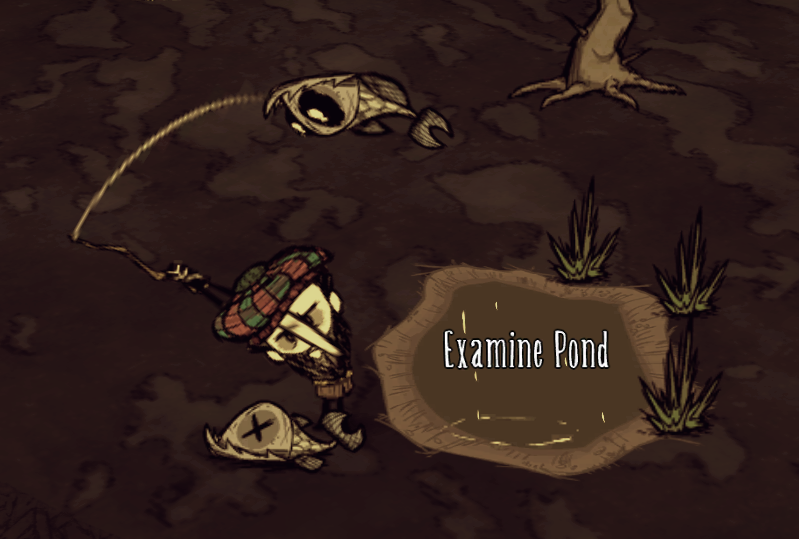
\includegraphics[width=\textwidth]{./Images/fishing}
  \caption{Wilson fishing in a pond.}
  \label{fig:fishing}
\end{figure}

As for the base camp, players tend to find places which can provide great quantities of meat since it will be the base of the players diet after the first few days.
Rabbit holes and Ponds are usually good places, as every day they spawn Rabbit and Frogs, respectively.
Additionally, ponds can be harvested with a Fishing Rod in order to collect fishes (Fig. \ref{fig:fishing}), that once cooked in a Crock Pot will provide a good Health regenerative.
Another important factor in the choosing of a base is the proximity to manure, a must have resource for the building of farms.

As the time passes and players start to have a steady supply of food items, the tendency is to start relocating other resources to make them more accessible.
Most players will dig up Grass Tufts, Sapplings, and Berry Bushes (they provide Grass, Twigs, and Berries, respectively) and plant them near the base camp, as seen in Fig. \ref{fig:basecamp-example}.
This will greatly increase a players collecting rate as all will be concentrated in an area around the players' camp, whereas the natural occurrence of such resources is usually sparse (occasionally, Berry Bushes and Grass Tufts will spawn in small clusters of nine elements near Pig Villages).
However, the relocation of Grass Tufts and Berry Bushes is usually troublesome as they require to be fertilized (using manure) in order to regrow.

\begin{figure}
  \centering
  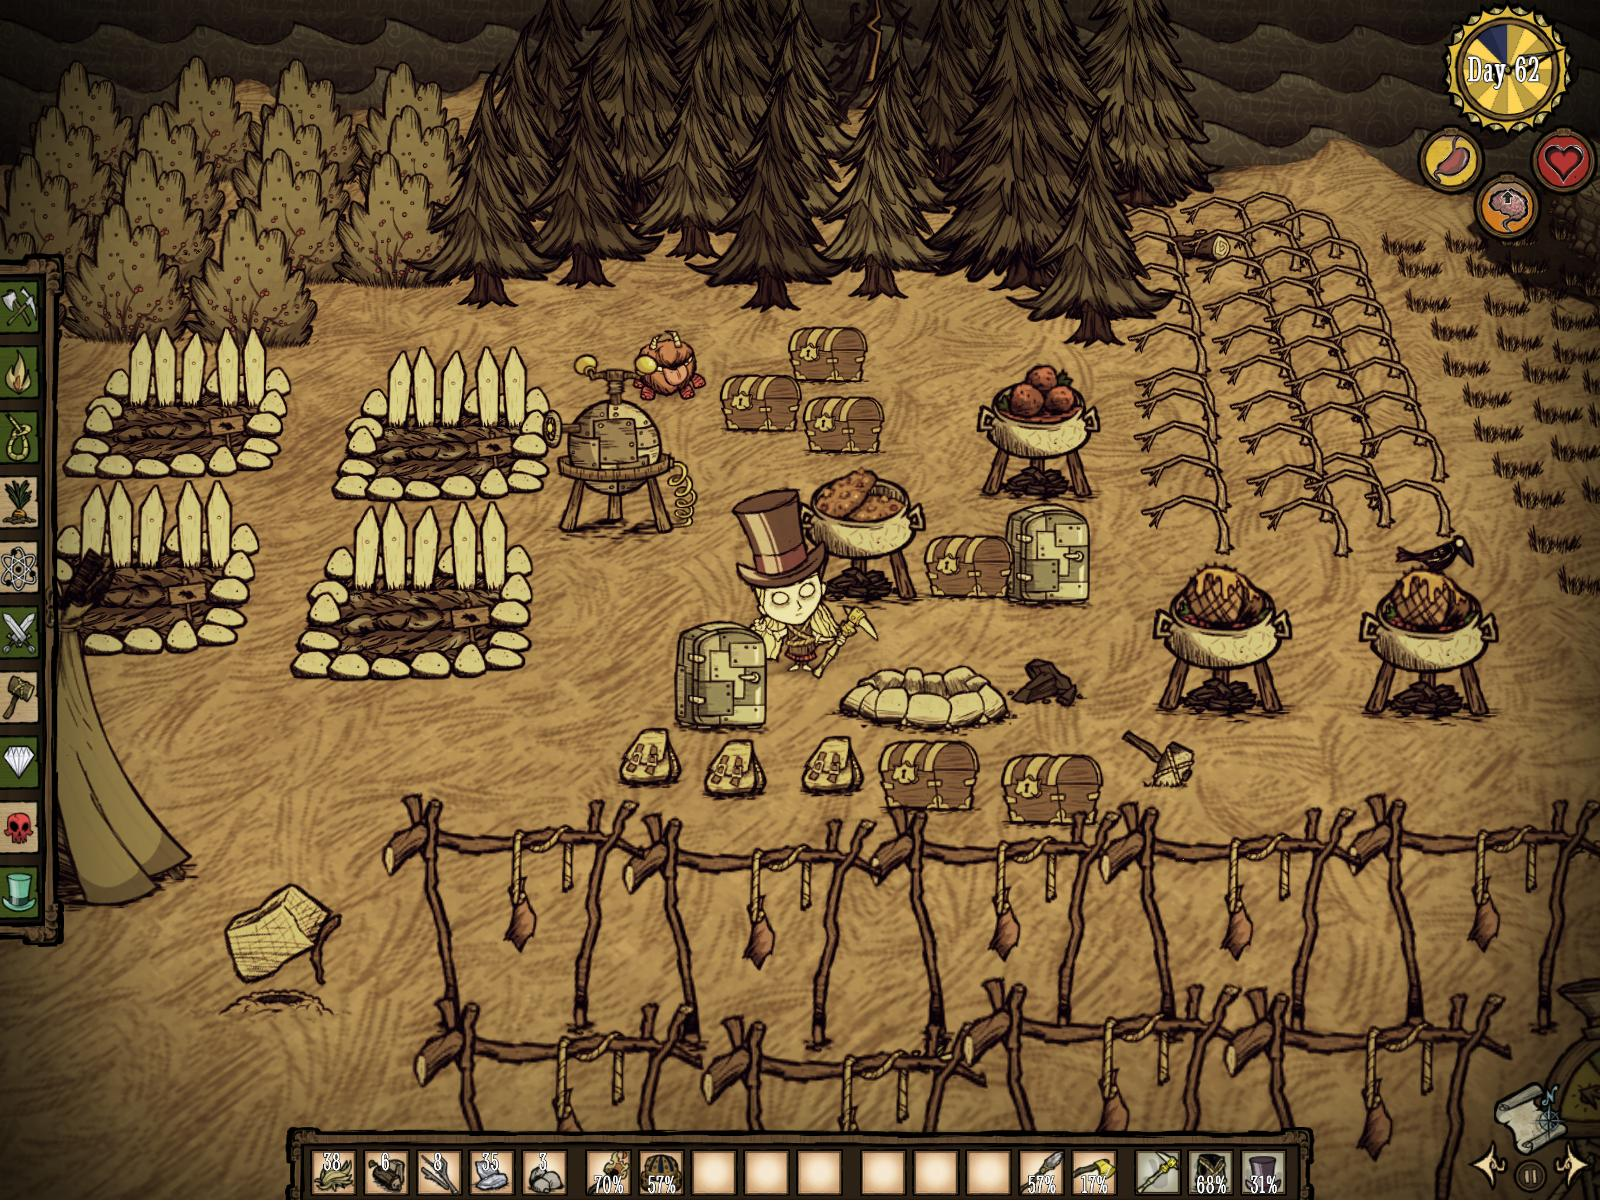
\includegraphics[width=\textwidth]{./Images/basecamp-example}
  \caption{An example of a base camp.}
  \label{fig:basecamp-example}
\end{figure}

In order to feed themselves, players use the Crock Pot to cook the food.
Crock Pots allow the elaboration of dishes that have several beneficial characteristics.
They can restore Hunger, Health and Sanity, with different dishes having different values, e.g. Fish Sticks restore a lot of Health but don't restores as much Hunger while the Meaty stew does the opposite.
For the cooking of dishes players use meats and vegetables.
The later is often obtain from farms, hence their presence in a players' base camp.

The base camp will usually be composed by a Science Machine or an Alchemy Engine (an improved version of the Science Machine), Farms, Drying Racks (used to dry meat which can them be stored for a longer period), Crock Pots, Chests (used to store items), clusters of Tress, Grass Tufts, and Saplings, and one or more Firepits.

As said before, if players stand in complete darkness for too much time, Charlie, the antagonist of the game, will attack and kill the player.
By standing next to a source of light, like a campfire, the player avoids being attacked by Charlie.

\section{Closing Remarks}

\noindent We've now thoroughly explored \ac{DST} game mechanics and frequently faced adversities.
A player's main concern is to keep the character's stats balanced throughout the game and find ways to survive the dangers each season brings.
To keep a steady supply of food and protection from the elements is as important as defending themselves from the monsters that will try to kill them.

To wrap up this chapter, bellow is a list of the core game mechanics with a small description.
This list represents a compilation of key aspects we have to take into account while making an \ac{NPC} for \ac{DST}.

\begin{description}
	\item[\textbf{Health}] \hfill \\ When it reaches zero a character dies. It can be replenished by certain items and by eating appropriate food and will be lost while fighting and when in extreme conditions of temperature.
	\item[\textbf{Hunger}] \hfill \\ Will cause a character to start losing health when it reaches zero. It will gradually decrease over time and can be increased by eating food.
    \item[\textbf{Sanity}] \hfill \\ Represents the mental state of the character. Certain conditions will cause it to decrease (e.g. fighting or standing in the dark) while others can cause it to increase (e.g. eating certain foods or being around befriended \textit{pigmen}). When near zero will provoke hallucinations that can attack the character. 
	\item[\textbf{Temperature}] \hfill \\ In cases of extreme cold or heat the character will start to lose health over time. It can be kept in check with the use of craftable items like clothes and fires.
	\item[\textbf{Wetness}] \hfill \\ As the character gets herself wet it can drop held items, food in the inventory will spoil faster, and her temperature will also decrease. The use of umbrellas and appropriate clothing will prevent the wetness level from rising.
    \item[\textbf{Darkness}] \hfill \\ When in complete darkness a character will be attacked by the darkness creature. It is important to stay near a source of light during the night.
    \item[\textbf{Fighting}] \hfill \\ Either as a means of defense or of gathering food, fighting is a core game mechanic without which survival is impossible.
\end{description}
% If Printing on DOUBLE SIDED pages, the second page should be white.
% Otherwise, comment the following command:
\cleardoublepage
%
%Chapter 4
% #############################################################################
% This is Chapter 4
% !TEX root = ../main.tex
% #############################################################################
% Change the Name of the Chapter i the following line
\fancychapter{Conceptual Model}
\cleardoublepage
% The following line allows to ref this chapter
\label{chapter:conceptual-model}


\noindent In this chapter we present a conceptual representation of our work.
Throughout this chapter we will describe each of the components of the model and its expected behaviour.
By the end of this chapter, the transition from the model, presented here, to the implementation, presented in Chapter \ref{chapter:implementation}, should be clear. 

In Figure \ref{fig:model} we can see several different modules and concepts.
The presented decoupling between the agent's \ac{AI} and the agent's embodiment, allows us to consider the use of different \ac{AI} techniques and different survival games.

Do notice that, despite the fact that the agent's \ac{AI} is represented outside the visual representation of the survival game, it needs not be the case.
Both concepts can be as tightly or as loosely coupled as needed for each different implementation.

Nonetheless, the Survival Game will need to provide ways for an \ac{NPC} to interact with the world, both by collecting information of the world using sensors and by making changes to the world through the use of actuators.
The \ac{NPC} will then extract the necessary perceptions about the world and, via a specified channel of communication, send them to the appropriate \ac{AI}.
The \ac{AI} will then perceive the received perceptions.
Whenever necessary, the \ac{AI} must emit actions that will be executed by the \ac{NPC} via the use of its actuators.
Throughout this execution, a Logger component will register all the executed actions, their outcome, and all the perceptions sent to the \ac{AI}.

\begin{figure}
  \centering
  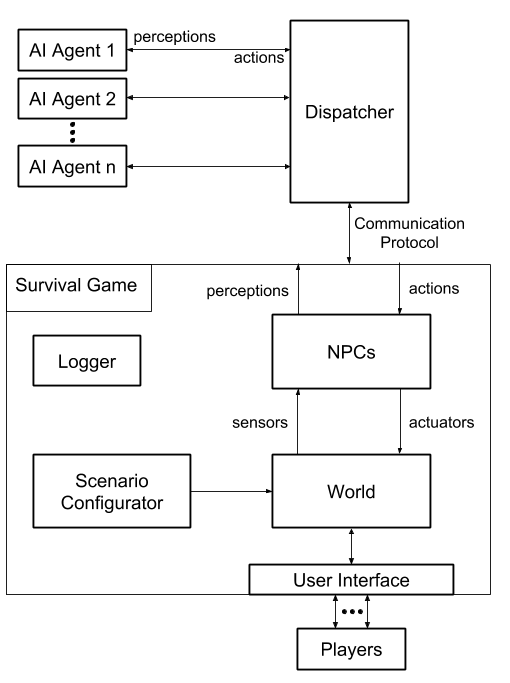
\includegraphics[width=\textwidth]{./Images/model}
  \caption{The proposed conceptual model.}
  \label{fig:model}
\end{figure}

Now that we've explored the general flow of the model, we'll describe each of its components in detail.

\begin{description}
	\item[\textbf{AI Agents}] \hfill
    
    This represents the \ac{AI} that will effectively control an \ac{NPC}.
    It is responsible for receiving perceptions and make decisions.
    It must be able to handle behaviour decisions and non-behaviour related decisions (such as dialogue).
    
    This module will need to have reactive capabilities as well as strategic decision making.
    Due to their dangerous environments and sometimes monsters, survival games (and in specific Don't Starve Together) require the ability to handle unexpected events, e.g. when a monster comes to attack the character.
    Additionally, they also require strategic decision making in order to better survive the world.
    The harshness of seasons will require that characters prepare ahead to better survive.
    
    Additionally, the capability for dialogue should be considered.
    Great part of player to \ac{NPC} interaction is based on dialogue, as such, this module should be able to handle dialogues.
    
    \item[\textbf{Dispatcher}] \hfill
    
    This module represents a bridge between the \ac{AI} and the embodiments of agents, managing the creation and destruction of the necessary \ac{AI} modules in accordance with the existing embodiments (\acp{NPC}).
    It is responsible to direct each perception and action to the appropriate recipient, be it the \ac{AI} or the embodiment of the agent.
    
    \item[\textbf{Communication Protocol}] \hfill
    
    Only present for illustrative purposes, the communication protocol is the bridge where perceptions and actions travel back and fort.
    This can be a simple local method invocation or a more complex communication system such as a remote method invocation over the network.
    
    Preferably the former, which presents significant advantages: reduced response time, no worries about availability of external services, and no need to translate information between potentially different systems.
    But, in the case of the later, it must handle the translation of information between systems transparently.
    
    \item[\textbf{World}] \hfill
    
    The virtual world of the game.
    This is where all the characters (\acp{NPC} and player characters) actually live and must provide ways for the \ac{NPC}s to act upon it and perceive it.

    \item[\textbf{Scenario Configurator}] \hfill
    
    This is, ideally, a part of the survival game.
    It provides a simple set of configurations that a developer can specify to configure the scenario that will be executed.
    It can also incorporate some configurations for the \ac{AI} that will empower the \acp{NPC}.
    
    \item[\textbf{NPCs}] \hfill
    
    This module represents the embodiment of the agents.
    It will execute any actions on the world and collect the necessary perceptions which in turn are sent to the \ac{AI}.
    
    \item[\textbf{Logger}] \hfill
    
    The Logger will be used to keep a registry of all the executed actions and their outcomes.
    It will also keep the registered perceptions of the \ac{NPC}.
    Although its representation puts it as a part of the game, this module can be independent from the game itself.
    
    \item[\textbf{User Interface and Players}]
    
    These modules are illustrative of the presence of players characters in the world.
    The survival game must accommodate the presence of several players that can play cooperatively or competitively and communicate with each other and the \acp{NPC}.
    
\end{description}


% If Printing on DOUBLE SIDED pages, the second page should be white.
% Otherwise, comment the following command:
\cleardoublepage
%
%Chapter 5
% #############################################################################
% This is Chapter 5
% !TEX root = ../main.tex
% #############################################################################
% Change the Name of the Chapter i the following line
\fancychapter{Implementation}
\cleardoublepage
% The following line allows to ref this chapter
\label{chapter:implementation}

\noindent To demonstrate our model, we've decided to implement it using a published commercial game, Don't Starve Together and a socially empowered model for agency with proofs given, \ac{FAtiMA} Toolkit.
During this chapter we will explain the inner workings of both Don't Starve Together and \ac{FAtiMA}, and then describe how we managed to implement our model.

In the end of this chapter we will also describe an \ac{NPC} that we published for the Don't Starve Together community, that can be played with.
After reading this chapter, the reader will have the necessary understanding to use our framework to develop an \ac{NPC} for Don't Starve Together.

\section{Don't Starve Together - The Survival Game}

\noindent As described in \ref{chapter:case-study-dst}, Don't Starve Together is a multi-player survival game, in which players either compete or cooperate in order to outlive the opponents and the world.
After reading that section, you will have an understanding of the challenges players face when playing the game.

However, we need to also understand the inner workings of the game.
For the remainder of this section we will explore the game's internal organization in detail, exploring how we can introduce our modifications into the game.

\subsection{Game Modifications}

\noindent In Don't Starve Together, modifications are introduced in the game through the use of the Steam Workshop, a public platform, where players can share modifications for games.
These modifications alter the original content of the game, adding new characters, creating new challenges, but mostly, altering the way the original game works.

In this particular case, the \textit{modders} (the name given to the players who share content on the platform) can alter the content of the game by writing Lua scripts\footnote{Lua is a scripting language and is currently the leading scripting language in games}, which are loaded by the game and modify its content (\href{https://www.lua.org/about.html}{https://www.lua.org/about.html}).
The game itself is already prepared to receive these \textit{mods} (the name given to the modifications published to the platform), and while some kinds of \textit{mods} are somewhat discouraged (like the addition of skins for the games characters), others are encouraged by the developers, who actively support the community in the game's forum.

For a \textit{mod} to be loaded by the game, it has to follow a specific structure and use of a set of helper functions to include the alterations.
As the game content is all written in Lua scripts (which are available to whomever owns a copy of the game)\footnote{The game engine is written in C++, but all the content and functionality is loaded through these Lua scripts}, \textit{modders} are encouraged to check the original game files in order to understand how the game works and how to implement their own changes.

\subsection{Entities}
\label{subsection:entities}

\noindent Everything that exists in the world of Don't Starve Together is represented as an Entity, from the character the player controls, to the sounds the player hears.
These, in turn, are instances of \textit{prefabs} that can be accessed and edited in the Lua scripts used to make the \textit{mods}.
It is important to note that each entity is uniquely identified by a six digit \ac{GUID}.

By specifying and configuring its \textit{components}, \textit{stategraphs}, and \textit{brains}, the \textit{prefabs} define every entity in the game.
Each of these parts represent something different: \textit{components} represent what an entity does; \textit{stategraphs} represent how it looks; and \textit{brains} represent how it behaves.

When a \textit{prefab} is defined, it also configures its \textit{components}, for example, in the definition of the \textit{prefab} ``wood", which contains the \textit{component} ``fuel", there is also the configuration of this \textit{component} that, in comparison to the \textit{prefab} ``charcoal", has a lower level of ``fuel".
Effectively, \textit{components} describe functionalities that a given entity can have, and how that functionality works.
When an entity, either by a player's command or the \textit{brain}'s command, does a chop action, it is the \textit{components} of the held axe that determine how this action will be executed and trigger the appropriate animations and events.

While \textit{components} can be reused throughout different \textit{prefabs} (with different configurations), \textit{brains} are defined on a per \textit{prefab} basis.
Both butterflies and spiders share the ``locomotor" \textit{component}, but have distinct moving behaviours.

When defining the \textit{prefab}, if it is meant to have behaviour, an instance of a \textit{brain} is also defined and attached to the \textit{prefab}.
However, not all \textit{prefabs} have autonomous behaviour, and those that don't, don't have a \textit{brain}.
The \textit{brain} itself is a Behaviour Tree that is attached to an entity, telling it what to do, leaving the part of how to do it up to the entity's \textit{components}.

Using the Lua scripts, a \textit{modder} can create \textit{components}, \textit{stategraphs}, and \textit{brains}.
These can then be attached to existing \textit{prefabs} or new ones, also created by the \textit{modders}.

\section{FAtiMA Toolkit - The AI Agent}

\noindent For the implementation of the \ac{AI} we chose to use \ac{FAtiMA} Toolkit \cite{dias:fatima-modular}, an agent creation toolkit.
As previously discussed in \ref{subsection:fatima}, \ac{FAtiMA} has been successfully used in several social scenarios (\cite{paiva:learning-by-feeling} \cite{rodrigues:i-can-feel-to} \cite{aylett:intercultural-empathy} \cite{correia:sueca}), making it the best choice for our implementation.

In this section, we present the Authoring Tools available to work with the toolkit.
Throughout this section, we will use the term developer to refer to someone who uses the FAtiMA-Toolkit to create agents.

\subsection{The Authoring Tools}

\begin{figure}
  \centering
  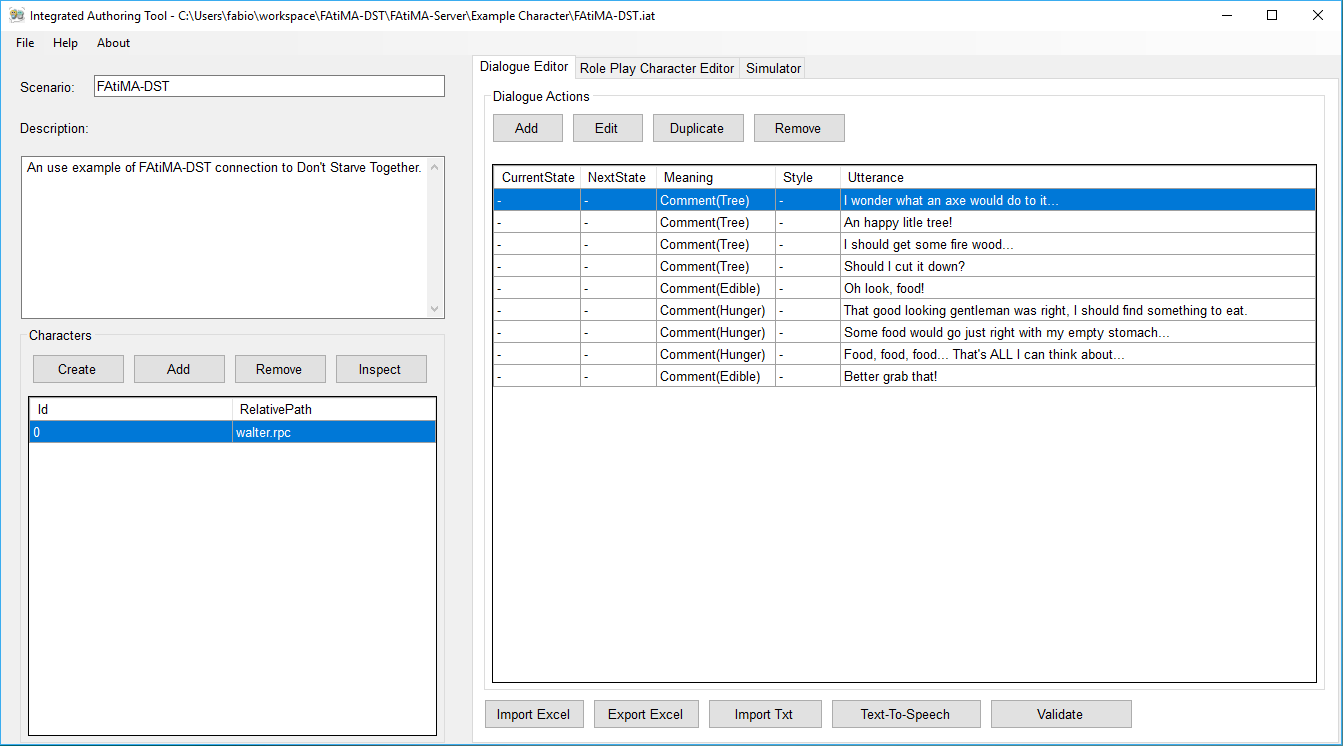
\includegraphics[width=\textwidth]{./Images/iat-interface}
  \caption{The Integrated Authoring Tool for \ac{FAtiMA} Toolkit.}
  \label{fig:iat-interface}
\end{figure}

\noindent The easiest way to develop a character with \ac{FAtiMA} Toolkit is by using the provided Authoring Tools.
Every implemented asset (described in \ref{subsection:fatima}) comes with a \ac{GUI} Tool which provides facilities to help develop a character.

The main tool is the \ac{IAT}, which can be seen in Figure \ref{fig:iat-interface}.
Through the \ac{IAT}, developers can access every other asset to develop their agents.
Developers can create dialogues, \acp{RPC} (and its components: Emotional Decision Making, Emotional Appraisal, etc.), run a chat simulator, and simulate and inspect \acp{RPC}.

In Figure \ref{fig:iat-interface} a set of dialogues from the example provided with our platform, Walter, can be seen.
The developer can use the example provided to create her own \acp{RPC}, and then use the Authoring Tools to test them.
The \ac{RPC} Inspector gives developers the possibility to provide a set of events that will be perceived by the \ac{RPC}.
The developer can then execute the contained scenario to see the emotional appraisal and decision processes in action.

\section{Putting it together}

\noindent Now that we have explored both the game used as a scenario and the technology used to control the characters, its time to look at how we connected both.
For the rest of this section, we'll present the implementation of the framework, explaining in full detail the decisions made.

The implementation itself consists in two modules: FAtiMA-DST, a Don't Starve Together \textit{mod}; and FAtiMA-Server, a C\# console application.
Both these modules have been made publicly available on the Github repository \href{https://github.com/hineios/FAtiMA-DST}{https://github.com/hineios/FAtiMA-DST}.
In the repository there is also a guide to help anyone develop an \ac{NPC} for Don't Starve Together.
As shown in Figure \ref{fig:implementation}, the communication between the two modules is made using \ac{HTTP}, which transfers \ac{JSON} objects back and forth.

The choice of using \ac{HTTP} communication arouse from a limitation we found while developing the initial proof of concept for this implementation.
Initially, we considered importing the \ac{FAtiMA} Toolkit directly, as the loading of C\# \ac{DLL} files into a Lua interpreter is possible.
However, as a security measure, the Lua interpreter embedded in \ac{DST} blocks any importation of external libraries.
The inclusion of malicious libraries through the Steam Workshop would be a major security issue for both the company and the players.

As alternatives, we considered using textual files or a relational database that would act as a proxy between the modules, but we finally decided to use an \ac{HTTP} connection as the game provided an easy way to make requests and register callback functions to handle the responses.
Due to the client-server nature of \ac{HTTP} however, the FAtiMA-DST module continuously makes \ac{HTTP} requests with \ac{JSON} encoded data to the FAtiMA-Server module, which handles these requests yielding an appropriate response (also \ac{JSON} encoded).
As a data-interchange format, \ac{JSON} provides the necessary abstraction to exchange information between C\# objects and Lua tables.

\begin{figure}
  \centering
  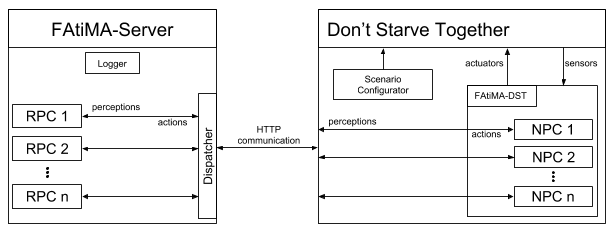
\includegraphics[width=\textwidth]{./Images/implementation}
  \caption{A graphical representation of the implementation.}
  \label{fig:implementation}
\end{figure}

\subsection{FAtiMA-Server}

\noindent The FAtiMA Toolkit is written in C\# and published as a set of DLL libraries.
Taking this into account, we decided to implement a simple server in C\#, capable of handling the \ac{HTTP} requests made by FAtiMA-DST \textit{mod}.
This server contains a list of Role Play Character Assets that are uniquely linked with the agents running on the scenario.
Each request the server handles has an entity's (\ac{NPC}) \ac{GUID}, which is used to also identify a Role Play Character Asset.

Additionally, requests are divided into three categories: perceptions, events, and decisions.
Perception requests contain information on the \ac{NPC}'s state and field of vision, and happen periodically.
Event requests contain information on relevant world events, and happen whenever an event is triggered.
Decision requests trigger the decision process that tells the \ac{NPC} what to do, and happen periodically.

If we consider the flow of information, the first two types (perception and event requests) represent a flow of information from the embodiment to the \ac{AI}, while the third (decision requests) represents a flow of information from the \ac{AI} to the embodiment.

When received, perception requests are translated into a series of Property-Changed events, that update the \ac{RPC}'s Knowledge Base.
Event requests will be translated to Action-End events and decision requests will trigger the \ac{RPC}'s decision process for the appropriate layer.

It is important to notice the limitations of using \ac{HTTP} as the method of communication.
This form of communication makes it impossible for the \ac{AI} to give direct actions to the embodiment, as we cannot send messages from the server to the client, only respond to client's requests.
As such, we have to rely on periodic requests made by the embodiment that will cause the \ac{AI} to make a decision and respond with an action.

\subsection{FAtiMA-DST}

\noindent This module was implemented as a \textit{brain} for \ac{DST} and is responsible to send perceptions to FAtiMA-Server and execute the actions it returns.
To achieve this, it sends a perception request to FAtiMA-Server two times a second, a decision request for behaviour every one and a half second, and a decision request for dialogue every ten seconds.
The values were tested and tweaked for the best compromise between behaviour and performance.

To send the perceptions to the FAtiMA-Server, it counts with a set of helper functions that extract the necessary information from surrounding entities.
A set of listeners relay information about events to the FAtiMA-Server, and a Behaviour Tree executes actions received from the FAtiMA-Server.
For a complete list of beliefs check Tables \ref{tab:state-beliefs} and \ref{tab:world-state-beliefs} and for actions refer to the Appendix \ref{appendix:A}

The Behaviour Tree makes use of the built-in Buffered Actions to execute the actions.
This provides a layer of abstraction over actions to handle all the locomotion details and appropriate verifications (e.g. it is only possible to chop a tree if an axe is held).

To handle the FAtiMA-Server commands, the tree contains two nodes: a node that executes actions (via buffered actions), and a node that handles the special behaviour of wandering.
The handling of dialogue is independent from the behaviour and is executed immediately without making use of the behaviour tree.

\section{Creating Walter}

\noindent As an example \ac{NPC}, we've implemented a model based agent to demonstrate how one could use the set of available beliefs to create behaviour.
This example only makes use of FAtiMA's Dialogue Manager and Emotional Decision Making assets.
%Using the provided examples from the toolkit and this example, developers will be able to create more complex \ac{NPC}s by making use of these and other assets.

This example has been published to the Steam Workshop in the form of an \ac{AI} companion, an \ac{NPC} named Walter \footnote{The \textit{mod} public page can be found in this link: \href{http://steamcommunity.com/sharedfiles/filedetails/?id=1339264854}{http://steamcommunity.com/sharedfiles/filedetails/?id=1339264854}}.
On the \textit{mod}'s public page, a set of instructions can be found on how to run the character.
The page also contains links to the public repository where all the code for this framework can be found.

% For the remainder of this section we will describe in detail the currently available beliefs and actions and how can these be used to create a \ac{NPC} using Walter as an example.

% \subsection{Beliefs}

The current set of beliefs available can be divided into two groups: character's state beliefs and world's state beliefs.
The complete listing of the beliefs is presented in tables \ref{tab:state-beliefs} and \ref{tab:world-state-beliefs}.
Most of them are self explanatory, but others require some explanation.

\begin{table}[htb]
	\centering
    \caption{Character's state beliefs}
    \label{tab:state-beliefs}
    \begin{tabular}{ | p{0.35\linewidth} | p{0.6\linewidth} | }
        \hline 
        \textbf{Belief} & \textbf{Description} \\ \hline \hline
        \texttt{Health([name]) = [value]} & Describes the agent's (\textit{name}) health \\ \hline
        \texttt{Hunger([name]) = [value]} & Describes the agent's (\textit{name}) hunger \\ \hline
        \texttt{Sanity([name]) = [value]} & Describes the agent's (\textit{name}) sanity \\ \hline
        \texttt{Moisture([name]) = [value]} & Describes the agent's (\textit{name}) moisture level \\ \hline
        \texttt{Temperature([name]) = [value]} & Describes the agent's (\textit{name}) temperature \\ \hline
        \texttt{IsFreezing([name]) = [bool]} & Describes if the agent (\textit{name}) is taking damage from extreme cold \\ \hline
        \texttt{IsOverheating([name]) = [bool]} & Describes if the agent (\textit{name}) is taking damage from extreme hot \\ \hline
        \texttt{IsBusy([name]) = [bool]} & Describes if the agent (\textit{name}) is currently executing any action \\ \hline
        \texttt{PosX([name]) = [value]} & The agent's (\textit{name}) current X position \\ \hline
        \texttt{PosZ([name]) = [value]} & The agent's (\textit{name}) current Z position \\ \hline
        \texttt{InLight([name]) = [bool]} & Defines if the agent (\textit{name}) is in the light or darkness \\ \hline
        \texttt{InSight([GUID]) = [bool]} & What the agent (\textit{name}) is currently seeing \\ \hline
        \texttt{InInventory([GUID]) = [bool]} & What the agent (\textit{name}) has in his inventory \\ \hline
        \texttt{IsEquipped([GUID]) = [bool]} & What the agent (\textit{name}) has equipped \\ \hline
    \end{tabular}
\end{table}

\begin{figure}
  \centering
  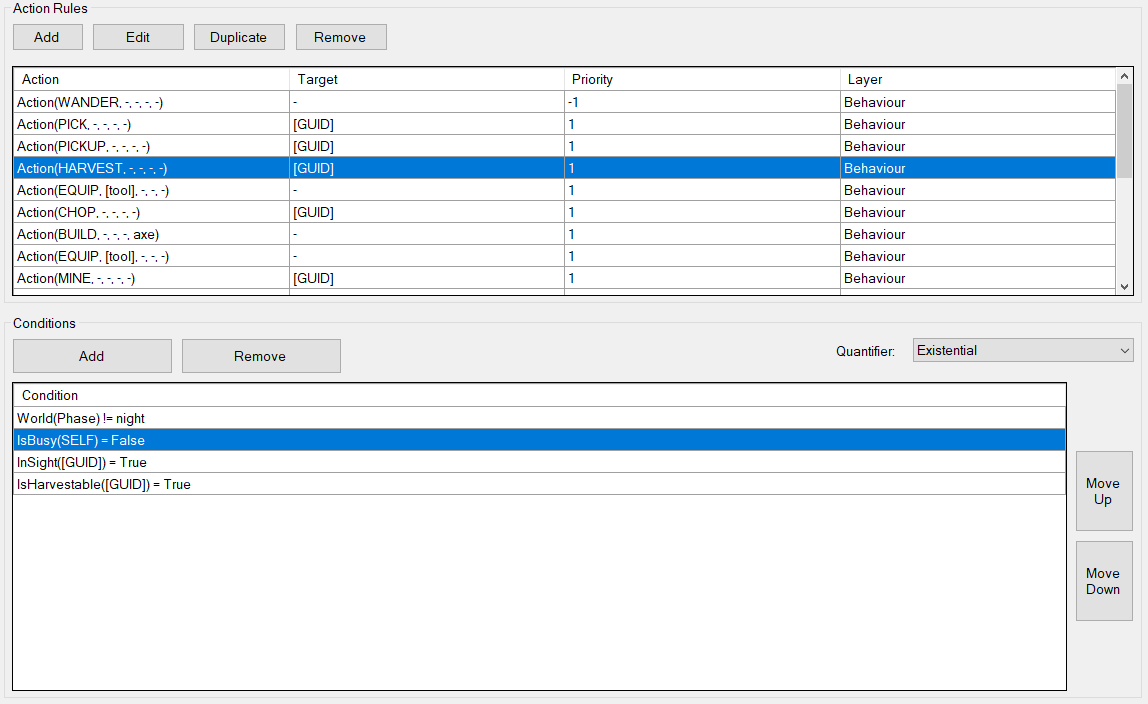
\includegraphics[width=\textwidth]{./Images/isbusy-example}
  \caption{Walter's \texttt{HARVEST} action.}
  \label{fig:harvest-example}
\end{figure}

The \texttt{IsBusy} belief is used to represent if the \ac{NPC} is executing an action.
As the implementation stands, if an action is received by FAtiMA-DST, the \ac{NPC} will immediately execute that action.
This allows for reactive behaviour and prevents the overlap of actions with equal priority.

The developer should use this belief as a condition for actions, as shown in Figure \ref{fig:harvest-example}, and omit this condition for actions that should be executed even if another one is being executed, as shown in Figure \ref{fig:equiptorch-example}.
In this example, equipping the torch can overlap other actions as it represents a case of life and death for the \ac{NPC} (being in the dark will get the \ac{NPC} dead).

\begin{figure}
  \centering
  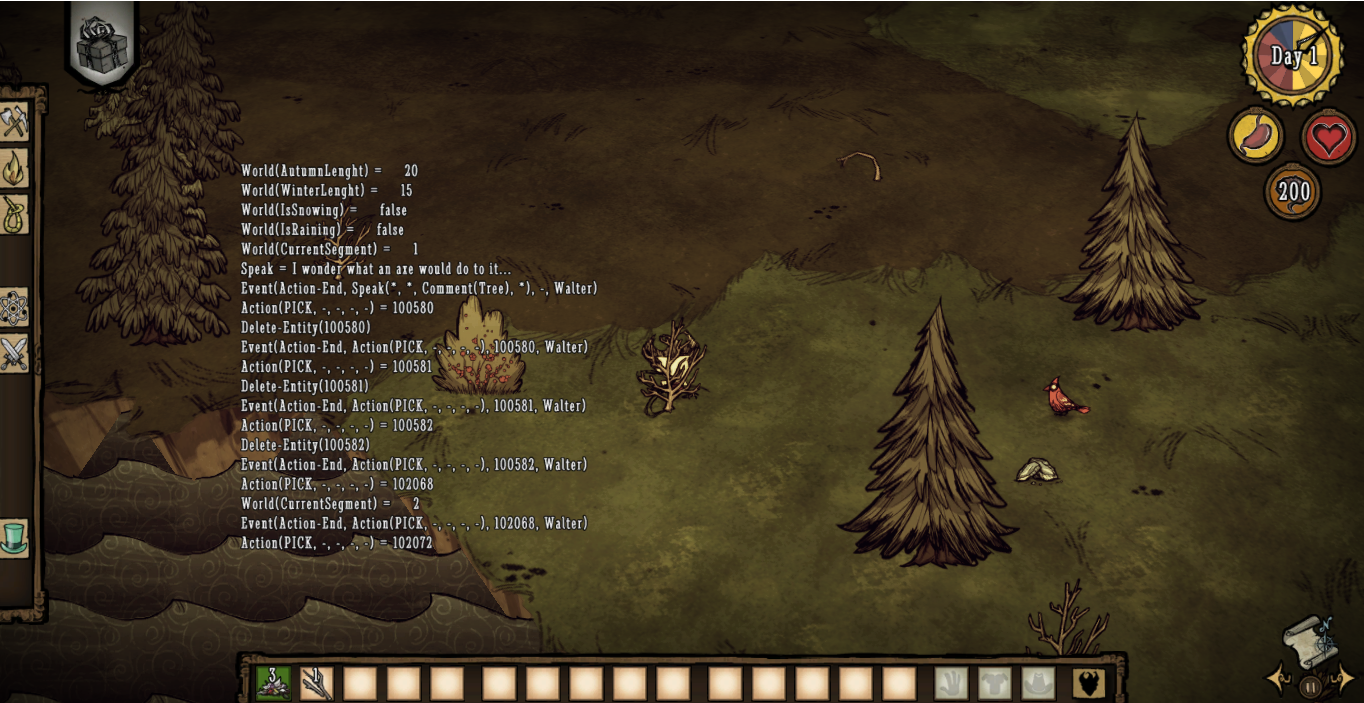
\includegraphics[width=\textwidth]{./Images/action-example-with-debug}
  \caption{Walter executing a \texttt{PICK} action with debug information being displayed in an overlay.}
  \label{fig:action-example-with-debug}
\end{figure}

\texttt{InLight}, \texttt{InSight}, and \texttt{InInventory} are in fact beliefs about entities.
However, they are presented here as they represent the state of entities in relation to the \ac{NPC}.
For example, Walter will only try to harvest any given entity if it is in sight, as shown in Figure \ref{fig:harvest-example}.
The use of these three beliefs is highly recommended when the action requires interaction of the \ac{NPC} with other entities.
The \ac{NPC} should not try to directly pick or pick up entities that she cannot see as they may no longer exist.

Do note that most of these beliefs require the agent's name.
While defining the Decision Making Asset rules, the special keyword \texttt{SELF} should be used for this purpose.
In Figure \ref{fig:action-example-with-debug} we can see the \ac{NPC} executing an action with some debug information being displayed in an overlay.

\begin{figure}
  \centering
  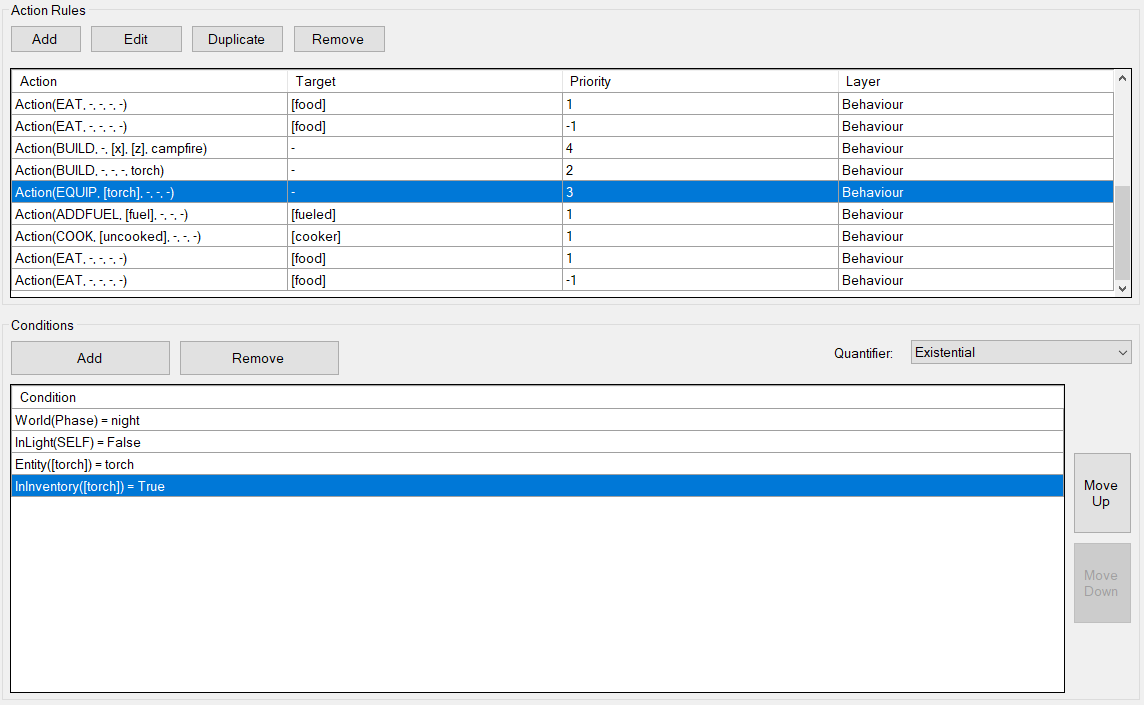
\includegraphics[width=\textwidth]{./Images/ininventory-example}
  \caption{Walter's \texttt{EQUIP} torch example.}
  \label{fig:equiptorch-example}
\end{figure}

\begin{table}[htb]
	\centering
    \caption{World's State beliefs}
    \label{tab:world-state-beliefs}
    \begin{tabular}{ | p{0.35\linewidth} | p{0.6\linewidth} | }
        \hline 
        \textbf{Belief} & \textbf{Description} \\ \hline \hline
        \texttt{Entity([GUID]) = [prefab]} & Defines an entity \\ \hline 
        \texttt{Quantity([GUID]) = [quantity]} & Defines how big is the stack (\textit{quantity}) of a given entity \\ \hline 
        \texttt{IsCollectable([GUID]) = [bool]} & True if the given entity is pickable (collect natural resources). \textit{PICK} action \\ \hline 
        \texttt{IsCooker([GUID]) = [bool]} & True if the given entity can cook other entities. \textit{COOK} action \\ \hline 
        \texttt{IsCookable([GUID]) = [bool]} & True if the given entity can be cooked. \textit{COOK} action \\ \hline 
        \texttt{IsEdible([GUID]) = [true]} & True if the entity may be eaten by the curent character (it takes into account the character's diet). \textit{EAT} action \\ \hline 
        \texttt{IsEquippable([GUID]) = [bool]} & True if the given entity may be equipped. \textit{EQUIP} action \\ \hline 
        \texttt{IsFuel([GUID]) = [bool]} & True if the given entity may be used to fuel stuff. \textit{FUEL} action \\ \hline 
        \texttt{IsFueled([GUID]) = [bool]} & True if the given entity requires fuel to function. \textit{FUEL} action \\ \hline 
        \texttt{IsGrower([GUID]) = [bool]} & True if the given entity can be used to grow seeds. \textit{PLANT} action \\ \hline 
        \texttt{IsHarvestable([GUID]) = [bool]} & True if the given entity is ready to be harvested. \textit{HARVEST} action \\ \hline 
        \texttt{IsPickable([GUID]) = [bool]} & True if the given entity is pickable (pick stuff from the ground). \textit{PICKUP} action \\ \hline 
        \texttt{IsStewer([GUID])= [bool]} & True if the given entity can take other entities to cook recipes \\ \hline 
        \texttt{IsChoppable([GUID]) = [bool]} & True if the given entity is workable by an axe. \textit{CHOP} action \\ \hline 
        \texttt{IsDiggable([GUID]) = [bool]} & True if the given entity is workable by a shovel. \textit{DIG} action \\ \hline 
        \texttt{IsHammerable([GUID]) = [bool]} & True if the given entity is workable by a hammer. \textit{HAMMER} action \\ \hline 
        \texttt{IsMineable([GUID]) = [bool]} & True if the given entity is workable by a pick. \textit{MINE} action \\ \hline 
        \texttt{PosX([GUID]) = [value]} & Defines the X coordinate (\textit{value}) of an entity \\ \hline 
        \texttt{PosZ([GUID]) = [value]} & Defines the Z coordinate (\textit{value}) of an entity \\ \hline 
        \texttt{World(CurrentSegment) = [value]} & The current segment, ranges between 0 and 15 \\ \hline 
        \texttt{World(Cycle) = [value]} & Defines how many cycles (days) have passed since the start of the game \\ \hline 
        \texttt{World(Phase) = [value]} & Defines the phase of the day. \textit{value} can be: 'day', 'dusk', or 'night' \\ \hline 
        \texttt{World(PhaseLenght, [phase]) = [value]} & The current duration of the day \textit{phase} in clock segments. The sum of all segments is always 16 \\ \hline 
        \texttt{World(Season) = [value]} & Defines the current season. \textit{value} can be: 'spring', 'summer', 'autumn', or 'winter' \\ \hline 
        \texttt{World(SeasonProgress) = [value]} & A value between 0 and 1 that defines the progress of the season \\ \hline 
        \texttt{World(ElapsedDaysInSeason) = [value]} & How many days have passed in the current season \\ \hline 
        \texttt{World(RemainingDaysInSeason) = [value]} & How many days are left to the end of the season \\ \hline 
        \texttt{World(SpringLength) = [value]} & Defines the current lenght of Spring \\ \hline 
        \texttt{World(SummerLength) = [value]} & Defines the current lenght of Summer \\ \hline 
        \texttt{World(AutumnLenght) = [value]} & Defines the current lenght of Autumn \\ \hline 
        \texttt{World(WinterLenght) = [value]} & Defines the current lenght of Winter \\ \hline 
        \texttt{World(IsSnowing) = [bool]} & True if it is snowing \\ \hline 
        \texttt{World(IsRaining) = [bool]} & True if it is raining \\ \hline 
        \texttt{World(MoonPhase) = [value]} & Defines the current moon phase. \textit{value} can be: 'new', 'quarter', 'half', 'threequarter', or 'full' \\ \hline 
	\end{tabular}
\end{table}

As far as world state beliefs go (described in Table \ref{tab:world-state-beliefs}), these are used to represent both the state of the world and entities present in the world.

Most beliefs used to describe entities coincide with the presence of certain \textit{components} (as described in \ref{subsection:entities}).
The use of these beliefs as conditions for the appropriate actions is highly encouraged as they will prevent the \ac{NPC} from trying to execute actions she cannot execute.

Walter will only harvest resources if the \texttt{IsHarvestable} belief is true, as depicted in Figure \ref{fig:harvest-example}.
This is also true for every other action present in Walter's decision rules.

Despite this, one can use the prefab of an entity as a condition, such as Walter does when equipping a torch (Figure \ref{fig:equiptorch-example}).
This will allow the creation of more refined behaviour.

Appendix \ref{appendix:A} contains two tables which have a comprehensive list of all available actions, Tables \ref{tab:actions-1} and \ref{tab:actions-2}.
Both tables also contain a brief description of every action, which along side the existing example of Walter, will help developers write their own behaviour rules.

\subsection{Dialogue}

\noindent As far as speech goes, the current framework has some limitations.
Currently, there is no two-way communication, meaning that, although the agent can speak (through the use of text), the players will not be able to respond.
In Figure \ref{fig:axe-dialogue} we can see the execution of a speak action by the agent while he is executing another action.

\begin{figure}
  \centering
  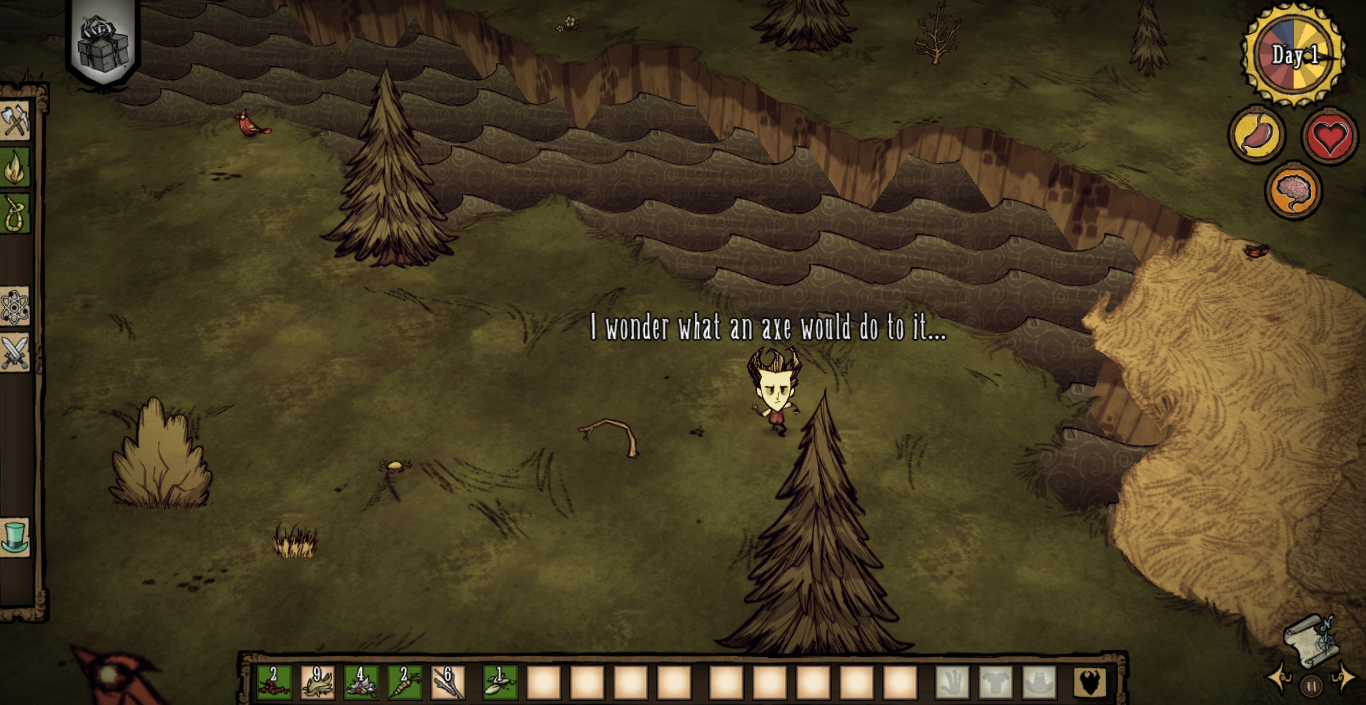
\includegraphics[width=\textwidth]{./Images/axe-dialogue}
  \caption{Example of speak action.}
  \label{fig:axe-dialogue}
\end{figure}

\begin{figure}
  \centering
  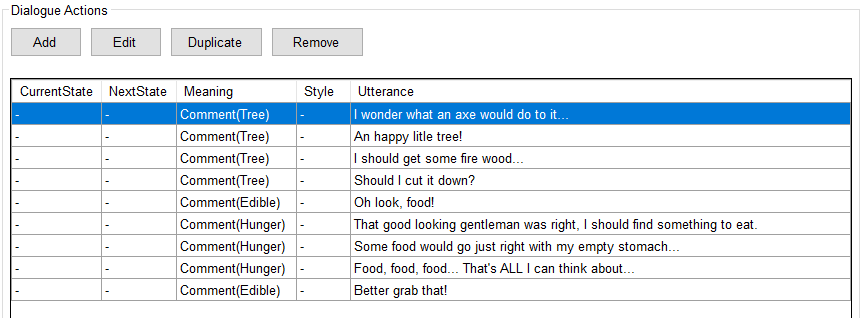
\includegraphics[width=\textwidth]{./Images/dialogue-example}
  \caption{Walter's available dialogues.}
  \label{fig:dialogue-example}
\end{figure}

To make an \ac{NPC} speak, the developer will need to create the available utterances using the Dialogue Editor as depicted in Figure \ref{fig:dialogue-example}.
Multiple utterances can be created with the same meaning, allowing for variety in the \ac{NPC}'s dialogue.
In Walter's example, several utterances have been added for each meaning.

To trigger these sentences, the developer also needs to add a rule with the appropriate layer to the decision making asset, as shown in Figure \ref{fig:dialogue-action-example}.
Here we can see, that in order for Walter to say a comment about hunger, his \texttt{Hunger} belief has to have a value lower than seventy.

\begin{figure}
  \centering
  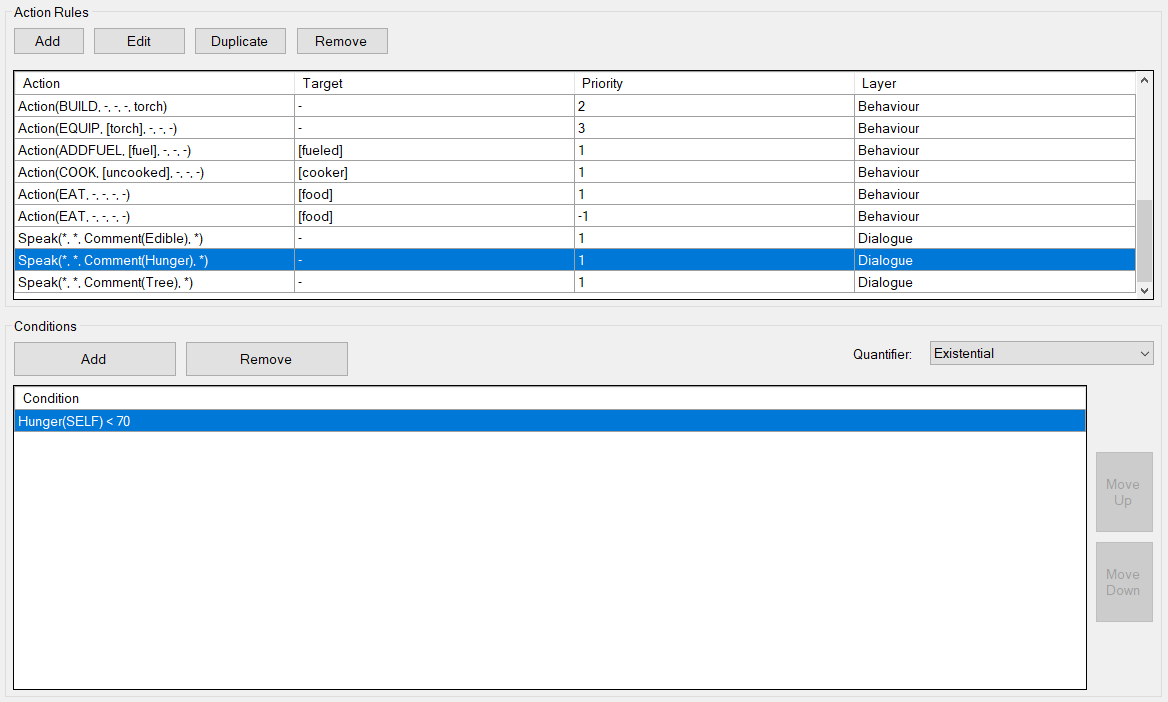
\includegraphics[width=\textwidth]{./Images/dialogue-action-example}
  \caption{Walter's dialogue action rule.}
  \label{fig:dialogue-action-example}
\end{figure}

The addition of these sentences allows players to better understand the \ac{NPC}'s decision process.
By stating some random utterances about its current state, we can transmit the characters state of mind to the players.
These sentences can also be used to transmit the \ac{NPC} emotional state, needs, and goals.

\section{Playing with Walter}

\begin{figure}
  \centering
  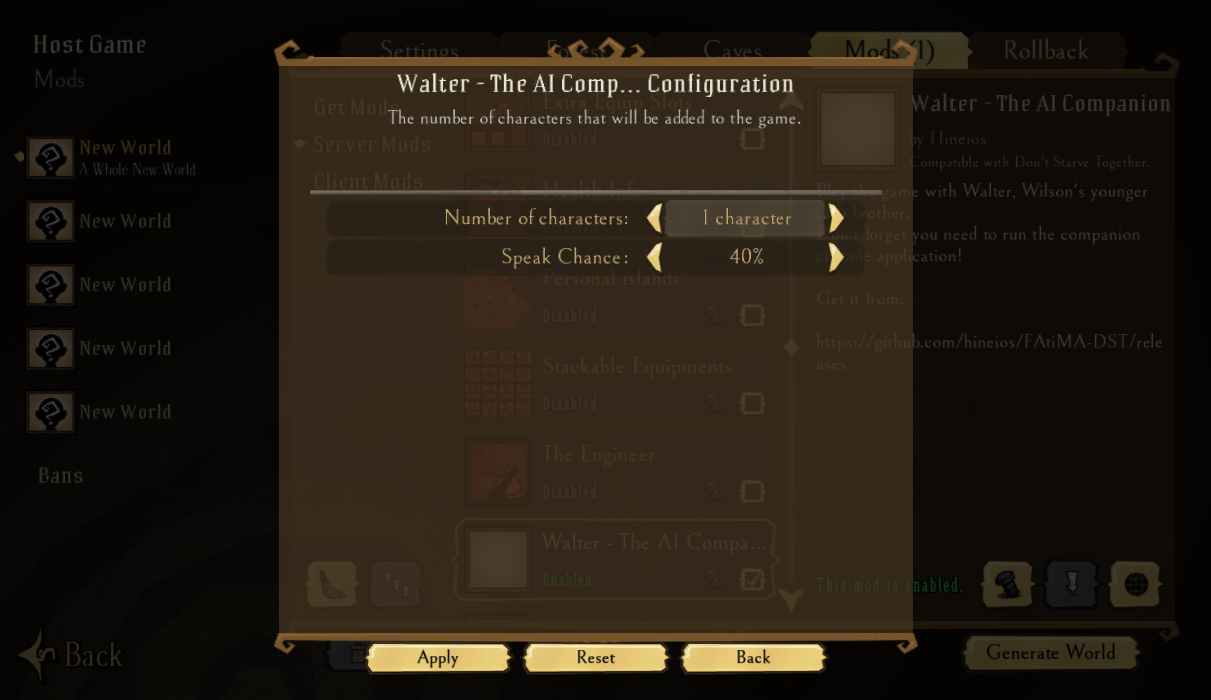
\includegraphics[width=\textwidth]{./Images/mod-config}
  \caption{Configuration screen for FAtiMA-DST.}
  \label{fig:mod-config}
\end{figure}

In order to run our framework, players will have to run FAtiMA-Server by launching the console application available at the public repository.
FAtiMA-Server will automatically listen to \ac{HTTP} requests on port 8080.
Then, before launching a game, the player will need to activate and configure the \textit{mod} as shown in Figure \ref{fig:mod-config}.
When the game is launched, the number of characters specified will spawn in the same place that players spawn.

\begin{figure}
  \centering
  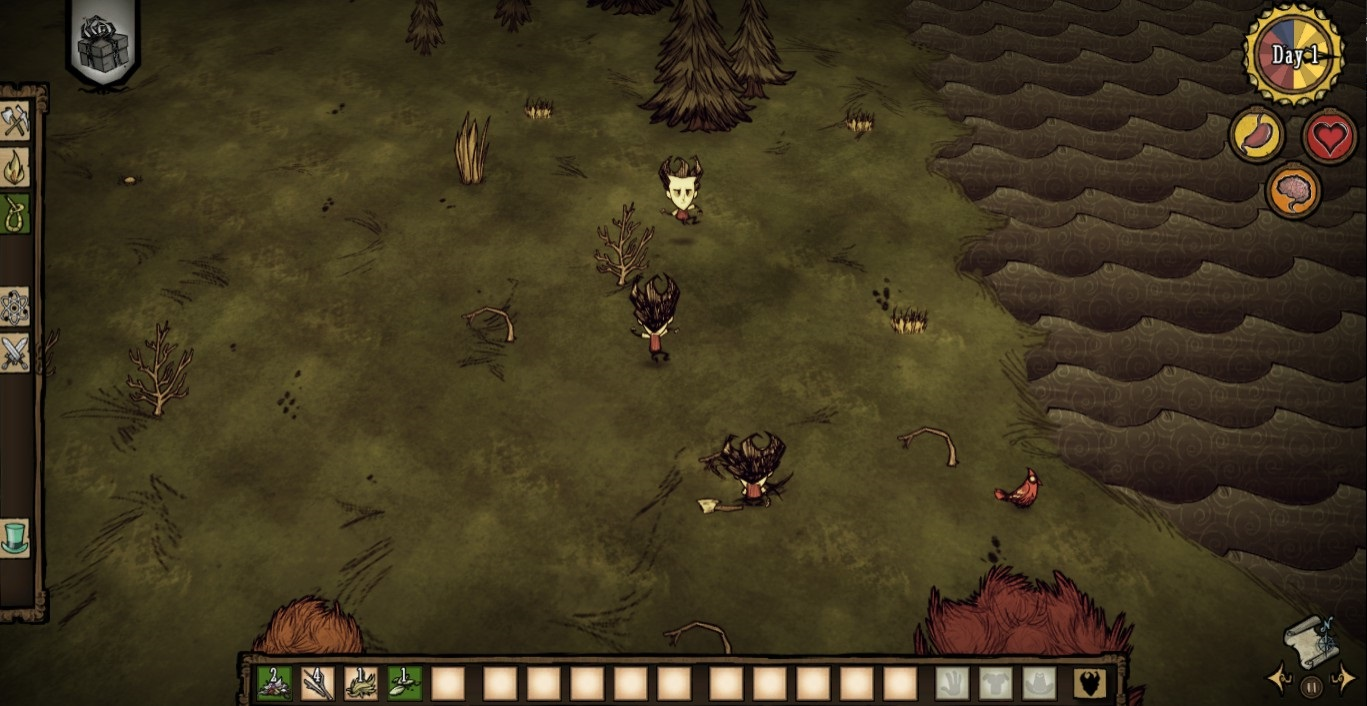
\includegraphics[width=\textwidth]{./Images/multiple-agents}
  \caption{A player (center) playing the \textit{mod} with two FAtiMA controlled characters (top and bottom).}
  \label{fig:multiple-agents}
\end{figure}

In Figure \ref{fig:multiple-agents}, we can see an example of a player playing the game with two \acp{NPC} being controlled by \ac{FAtiMA}.

% If Printing on DOUBLE SIDED pages, the second page should be white.
% Otherwise, comment the following command:
\cleardoublepage
%
%Chapter 6
% #############################################################################
% This is Chapter 6
% !TEX root = ../main.tex
% #############################################################################
% Change the Name of the Chapter i the following line
\fancychapter{Evaluation}
\cleardoublepage
% The following line allows to ref this chapter
\label{chapter:evaluation}

\noindent By the end of this project we've successfully implemented a framework that enables developers to use an agency model, \ac{FAtiMA}, to create \acp{NPC} for Don't Starve Together.
This was achieved through the implementation of a modification for \ac{DST} and a companion console application.
As contributions resultant from this work we also count with a tutorial for creating \acp{NPC} and an example \ac{NPC}.

For the remainder of this chapter we will talk about the published \textit{mod}, then we will talk about a use case of the framework, and will finish with a comparison between our example character and the work of an anonymous developer.

\section{Walter - The AI Companion}

\noindent As said before, the example character we created to demonstrate the framework has been published in the Steam Workshop.
At the time of writing, with 48 days of existence, the \textit{mod} counts with 738 unique viewers and 128 subscribers, as shown in Figure \ref{fig:walter-stats}.

While subscribers represent the number of people who've added the \textit{mod} to their game, it does not tells us how many of those have actually used the \textit{mod}.
The \textit{mod} also counts with 25 comments on the public page, mostly related to running the mod.

Although it has received no direct negative feedback, we believe that the necessity of running a separate console application has greatly impacted the community's acceptance and use of the \textit{mod}.
Additionally, to the best of our knowledge, no member of the community has used our framework to develop their own \acp{NPC}.

\begin{figure}
  \centering
  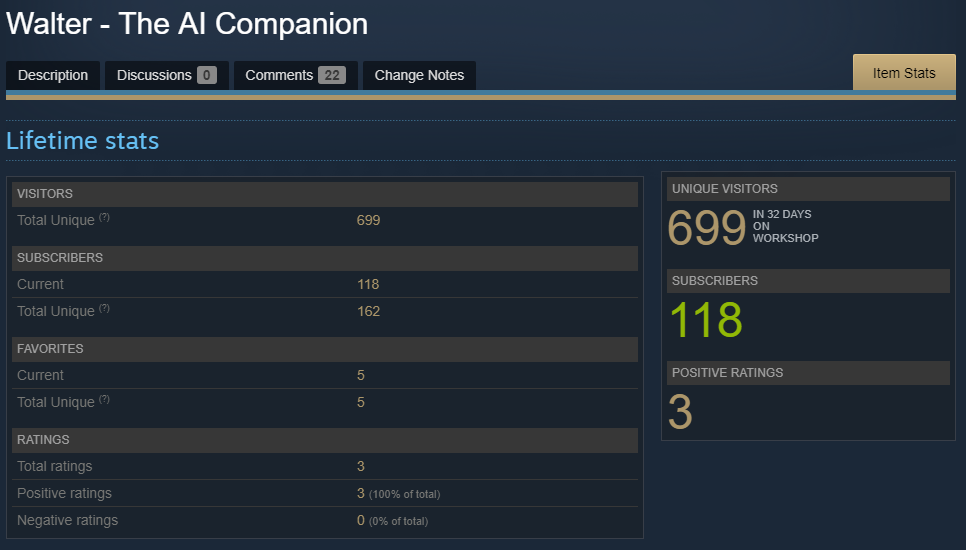
\includegraphics[width=\textwidth]{./Images/walter-stats}
  \caption{Walter - The AI Companion \textit{mod} lifetime stats.}
  \label{fig:walter-stats}
\end{figure}

\section{Monte Carlo Tree Search Project}

\noindent As part of the Artificial Intelligence for Games course taught at Instituto Superior Técnico, a group of three students used our framework for their final project.
The project consisted in the implementation of the \ac{MCTS} algorithm for the decision process of the agent.

Briefly, the \ac{MCTS} algorithm is based in a random exploration of a state space.
By randomly (and rapidly) collecting data of the space state, the algorithm will gradually improve its knowledge of what the best next move is.

Unlike many other algorithms, \ac{MCTS} does not run until an answer is found.
Instead, the usual approach consists in letting the algorithm run for some time (or a certain number of iterations) and then return the best possible action, in regard to the information collected so far.
The algorithm has proven to be especially good in problems where the space state has an high branching factor and many possible combinations, such as the Go game.

In this case, the implementation of the \ac{MCTS} algorithm was achieved through the use of \ac{FAtiMA}'s Dynamic Properties.
The created Dynamic Property, called \texttt{MCTS}, will use current knowledge base and apply the \ac{MCTS} algorithm.
The \ac{MCTS} algorithm was let run for two thousand iterations (about twenty seconds) before returning a plan to act upon.

One of the main difficulties found during this use case was related to the random exploration of the state space.
As Don't Starve Together does not provide a way to simulate the resulting state of applying actions and \ac{FAtiMA} did not have such functionality either (although it can now achieve this through the use of the World Model Asset), the group had to create their own simulator of the Don't Starve Together world.

This work, praises the versatility of our framework by demonstrating the ability to create a planning agent based on \ac{MCTS}.
Although the group had to struggle with the world simulation, the end result was an \ac{NPC} for \ac{DST} with planning capabilities.

\section{Walter vs. Artificial Wilson}

\noindent As a means of evaluating the created \ac{NPC}, we've run it and recorded how long it can survive.
Additionally, we compare it to an unpublished character for Don't Starve, Artificial Wilson.

Artificial Wilson, is the work of the anonymous \textit{modder} KingofTown and can be found in the public repository \href{https://github.com/KingofTown/DS-AI}{https://github.com/KingofTown/DS-AI}.

\subsection{Testing Conditions}

\noindent For each run of the characters, a new world was dynamically generated with equal sets of constraints for both characters.
The characters were then let run for as long as possible until their death.

As we said, Artificial Wilson was created for the original game, Don't Starve.
Therefore it is incompatible with Don't Starve Together because of the updates made to turn it into a multiplayer game.
However, the game mechanics and configurations remain the same.

As such, we can use the scenario configurator to generate equivalent worlds.
For this test, we considered the following restrains:

\begin{itemize}
	 \item \textbf{A world with no enemies}: all aggressive monsters have been removed from the game as well as the giants.
     \item \textbf{No random meteorological events}: apart from raining all other events have been disabled (like meteors,  frog rains, lightning storms, and wildfires).
     \item \textbf{No resurrection stones}: if the \ac{NPC} dies, it stays dead.
     \item \textbf{No matting season for \textit{beefalos}}: during this season these, normally pacific creatures, will attack any character on sight.
     \item \textbf{No modifications}: apart from the necessary ones for running both characters.
     \item \textbf{Only one \ac{NPC} and no players}: while in Don't Starve this does not apply, in Don't Starve Together the tests were run locally with no players present in the world.
\end{itemize}

These constrains will generate similar worlds for both Don't Starve and Don't Stave Together.
For each play-through of an agent, a new world is generated with these sets of constraints.
Each generated world is unique but complies to the specified set of constraints.

\subsection{The Results}

\noindent Each character has been run thirty times and the survival duration for each character is presented in Figures \ref{fig:days-survived-walter} and \ref{fig:days-survived-wilson}.

\begin{figure}
  \centering
  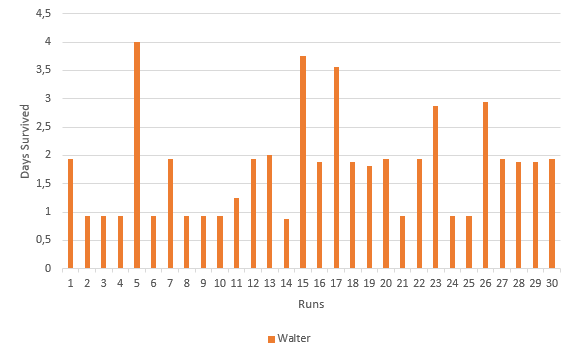
\includegraphics[width=\textwidth]{./Images/days-survived-walter}
  \caption{Days survived for Walter.}
  \label{fig:days-survived-walter}
\end{figure}

\begin{figure}
  \centering
  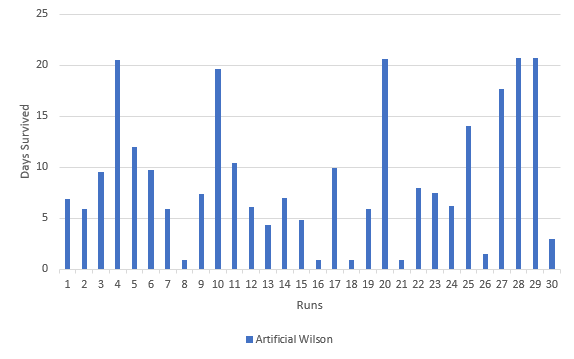
\includegraphics[width=\textwidth]{./Images/days-survived-wilson}
  \caption{Days survived for Artificial Wilson.}
  \label{fig:days-survived-wilson}
\end{figure}

\begin{figure}
  \centering
  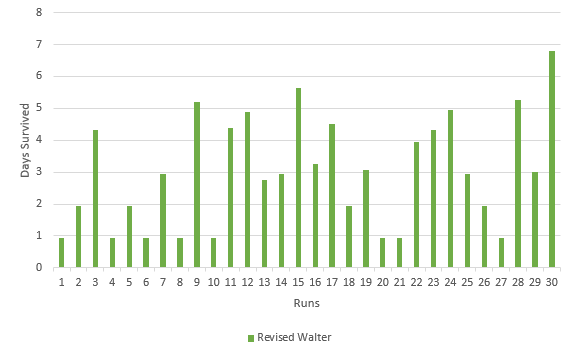
\includegraphics[width=\textwidth]{./Images/days-survived-walter-new-and-improved}
  \caption{Days survived for revised version of Walter.}
  \label{fig:days-survived-walter-new-and-improved}
\end{figure}

Walter survived, on average, one point eight days while Artificial Wilson survived, on average, eight point nine days.
The percentage difference of 132\% between both values can be explained by the detail put in each character's decision process\footnote{Percentage difference equals the absolute value of the change in value, divided by the average of the 2 numbers, all multiplied by 100. We then append the percent sign, \%, to designate the \% difference.}.

Walter is a model based agent with nineteen rules of decision.
Each of these rules has no decision process besides the character's ability to perform it (e.g. does the \ac{NPC} has an axe equipped to cut down a tree?, does it have the required ingredients to build a fire?).

Artifical Wilson is based on the built-in behaviour trees.
The final behaviour tree counts with over seventy nodes and dozens of helper functions.
Embedded in the \acp{NPC}'s decision process are some planning capabilities and resource management (e.g. the \ac{NPC} will ignore resources if she has already gathered enough of it), which Walter does not possess.

If we compare both characters to real human players, Walter has the ability of a newcomer who as never played the game, while Artificial Wilson could be compared to a returning player who played the game for a couple dozen of times\footnote{This comparison has been based on the writer's experience with the game}.

For each character we've recorded not only their survival time but also their cause of death.
In Table \ref{tab:cod} you can see a summary for both characters.

\begin{table}[htb]
	\centering
    \caption{Artificial Wilson, Walter, and Revised Walter cause of death summary.}
    \label{tab:cod}
    \begin{tabular}{ | p{0.18\linewidth} | p{0.1\linewidth} | p{0.18\linewidth} | p{0.1\linewidth} | p{0.18\linewidth} | p{0.1\linewidth} |}
        \hline 
        \multicolumn{2}{|c|}{Artificial Wilson} & \multicolumn{2}{|c|}{Walter} & \multicolumn{2}{|c|}{Revised Walter} \\ \hline 
        Cause of Death & Times & Cause of Death & Times & Cause of Death & Times \\ \hline
        Cactus & 2 & Darkness & 18 & Darkness & 17 \\ \hline
        Cold & 5 & Fire & 8 & Hunger & 13 \\ \hline
        Darkness & 10 & Hunger & 4 & & \\ \hline
        Hunger & 13 & & & & \\ \hline
    \end{tabular}
\end{table}

We can see that Walter died several times due to fire damage.
Upon analyzing its behaviour, we observed that this was due to the \ac{NPC}'s placement of campfires.
The reactive rules we've empowered Walter with, have no concern for the placement of structures.
As such, the \ac{NPC} would often build campfires in the middle of forests that would be set ablaze by the campfire. This, in turn, would cause the \ac{NPC} to die by fire.

In order to counteract this, we decided to disable the rule for building campfires.
Instead the agent relies on torches to illuminate itself through the night.
The results are presented in Figure \ref{fig:days-survived-walter-new-and-improved}.
The average surviving time for Walter increased from one point eight days to three days, which represents an increase of 66\%. 

%The problem with the placing of structures as also been considered for future work.
%An helper function that finds a suitable place for construction, near the position specified by the \ac{AI} would solve this and future problems related to structure placement.

\subsection{Notes on Character Behaviour}

\noindent We would like to note some aspects we found interesting from both character's behaviour.

While Artificial Wilson has a selective picking and manages his inventory, Walter's reactive behaviour lacks this features.
In fact, for runs that Walter was able to survive more that two, three days it became apparent that the lack of space in the inventory was a great hindrance.
Most of the time Walter would collect many items that would just occupy space in the inventory without ever using them.

Regarding the map exploration, Artificial Wilson would end up by exploring a lot more of the map than Walter.
This is directly related to the point discussed before.
By picking only what it needs, Artificial Wilson would move on to unexplored territories to find what it needed.
On the other hand, Walter would stay around the same place for extensive amounts of time.

This brings us to the third aspect we would like to discuss.
By staying on the same area, Walter would eventually deplete all the available resources.
This killed him most of the time, due to the lack of food or materials to make a torch for the night.
Artificial Wilson however, did not suffer from this problem as it roamed the world more extensively, being able to recollect certain resources that would regrow while it was exploring other parts of the world.
By comparison, Walter's decision making is too heavily focused on exploiting its available resources and providing a better exploration-exploitation balance could lead to better results.

% If Printing on DOUBLE SIDED pages, the second page should be white.
% Otherwise, comment the following command:
\cleardoublepage
%
%Chapter 7
% #############################################################################
% This is Chapter 7
% !TEX root = ../main.tex
% #############################################################################
% Change the Name of the Chapter i the following line
\fancychapter{Conclusion}
\cleardoublepage
% The following line allows to ref this chapter
\label{chapter:conclusion}

\noindent In this dissertation we've argued how in video games that are heavily dependent on interactions with \acp{NPC}, many of them are not socially aware and behave in a non-believable manner.

Firstly, we have looked at how the video game industry is currently making \acp{NPC} and concluded that the used techniques do not involve current frameworks and architectures for social agents.
The use of Behaviour Trees and Finite State Machines, the most commonly used techniques in today's industry, provide skilled game designers with the ability to create somewhat complex behaviour.
However, these techniques can quickly become an authoring burden.
Having to manage hundreds of behaviour nodes or states is no simple task.
Furthermore, grasping the context of social interaction will often be left out of the \ac{NPC}'s behaviour.

Focusing on survival games, we've noticed how these games will often lack the presence of \acp{NPC}, and when they are present, they can break the player's immersion by not being subject to the same rules as the players.
This, allied to the fact that many survival games rely on multiplayer interaction in order to keep interesting, has motivated us to create a platform that allows developers to create believable \acp{NPC} with interesting behaviour for survival games.

To achieve this, we had to explore what other platforms are currently available to develop \acp{NPC}. To the best of our knowledge there are no publicly available platforms that allow developers to create \acp{NPC} for survival games.
We've then decided to look into agent creation platforms and explored tools like \ac{JADE}, NetLogo, and PsychSim.
Although they represent good options for agent engineering and simulations they do not provide us with the necessary tools to solve our problem, the creation of believable \acp{NPC} in survival games.

In order to make believable \acp{NPC} we need them to possess certain human-like traits: social awareness, active goal pursuit, and reactivity, for example.
As such, the next step was to look at agency models that concern themselves with believability and social interaction without forfeiting reasoning and planning.
Versu, \ac{CiF}, and \ac{FAtiMA}, are all fully-fledged agency models, but we decided to use \ac{FAtiMA} due to its versatility and decision making capabilities.
By incorporating \ac{FAtiMA}'s capabilities into a commercial survival game we've been able to realize a platform that allows developers to create \acp{NPC} with social ability and planning capabilities.

We've chosen Don't Starve Together for its multiplayer nature, its ability to configure the world we play in, the possibility of including our own modifications to the game natively, and for its sanity mechanic.
A novelty among its peers, the sanity mechanic represents the character's mental health, another component that enhances the player's immersion by giving the character a human trait.

Then we implemented the \textit{mod}, FAtiMA-DST, and the console application, FAtiMA-Server, that allow us to run \ac{AI} powered \acp{NPC} in \ac{DST}.
As an example and proof of concept, we've also created Walter, a model based \ac{NPC} that was published in the Steam Workshop.

Additionally, the platform has been successfully used to implement a planning agent using the \ac{MCTS} algorithm.
By creating a new Dynamic Property, the developers were able to create an agent using \ac{FAtiMA} and run it in \ac{DST}.

In order to evaluate our work, we've compared our example agent, Walter, with Artificial Wilson, an agent created using the in-game's behaviour trees by an anonymous \textit{modder}.
Although Walter's performance is poor when compared to Artificial Wilson, the discrepancy can be justified due to the difference in the size of both implementations.
While Walter counts with nineteen rules of decision, Artificial Wilson counts over seventy nodes in its behaviour tree.

This dissertation provides the ground work for future developments in the creation of \acp{NPC} for survival games, in particular for Don't Starve Together.
It is our belief that with an equal effort, Walter's behaviour would at least match the performance of Artificial Wilson with the added value of social awareness, emotional responses, and active goal pursuit.

\section{Future Work}

\noindent As this work stands, it allows the creation of \acp{NPC} for Don't Starve Together.
However, the platform has great room for improvement.

\begin{itemize}
\item Two-way communication.
Currently, the platform allows the \ac{NPC} to talk and make remarks on the world.
However, the player is not able to respond and talk back to the \ac{NPC}.
Either by allowing chat responses or by adding an additional component to the game's interface, the interaction with the \ac{NPC} could be greatly improved.

\item Add more beliefs.
Expanding the character's available beliefs will enable us to create more complex behaviour.
However, only by adding behaviour to \acp{NPC}, will we understand which beliefs are effectively necessary.

\item Improve Walter.
As a proof of concept Walter plays its role as expected.
Nonetheless, Walter is a simple model based agent that does not make full use of \ac{FAtiMA}'s capabilities.
Although the framework is fully prepared to support \ac{FAtiMA}, the character does not benefit from all the capabilities \ac{FAtiMA} might grant to a virtual agent. By incorporating additional assets into the \ac{RPC}'s definition, like the Emotional Appraisal Asset or the Social Importance Asst, Walter could be further improved.

\item Reduce the burden of running FAtiMA's characters in \ac{DST}.
As it stands, players have to run a console application in parallel with the game for the platform to work properly.
It is our belief that by removing this requirement, more players would be able to play with \acp{NPC} that make use of our platform.
Ideally, this would be done by incorporating \ac{FAtiMA}'s \ac{DLL}s into the embedded Lua interpreter that \ac{DST} comes with.
However, this would require some sort of collaboration with the game developers, Klei Entertainment.
Alternatively, a public server could be set up to host the FAtiMA-Server component.

\item Add an additional layer of decision.
Players can express feelings through the use of gestures.
Gestures are animations that represent different states of mind the player may be feeling (some of the available gestures are ``annoyed", ``bye", ``angry", ``joy", ``dance", and ``sad").
The addition of this capability to the platform would be a great improvement as far as believability goes for created \acp{NPC}.

\item Add more composed actions to the platform.
Currently the only composed behaviour incorporated in the platform is the wander behaviour.
The addition of combat behaviour, utilization of chests, structure placement helpers, and others, would greatly improve an \ac{NPC}'s capabilities.

\item Different \acp{NPC} running different \acp{RPC}.
For each \ac{NPC} there should be an ability to specify the \ac{RPC} to be loaded.
This would enable the creation of richer scenarios by using characters with different characteristics, goals, reactions, dialogues, among others.

\end{itemize}

% If Printing on DOUBLE SIDED pages, the second page should be white.
% Otherwise, comment the following command:
\cleardoublepage
%
% -----------------------------------------------------------------------------
% BIBLIOGRAPHY
% Add the Bibliography to the PDF table of contents (not the document table of contents)
\pdfbookmark[0]{Bibliography}{bib}
% The bibliography style sheet
% Chose your preferences on the format of the entries and the Labels:

% IEEEtran: Used in general (recommended for IST Thesis)
%           Entries are labelled and sorted by appearance in the document
%           Labels are Numeric inside square brackets
\bibliographystyle{IEEEtran}

% Apalike:  Entries formatted alphabetically, last name first, with identation
%           Labels with Autor's Name and Year inside square brackets
%\bibliographystyle{apalike}

% Alpha:    Entries formatted with Autor's Name and Year, hanging identation
%           Labels with Autor's abbr. Names and Year inside square brackets
%\bibliographystyle{alpha}

% Acm:     Entries formatted with Autor's Name (small Caps), hanging identation
%          Labels are Numeric inside square brackets
%\bibliographystyle{acm}
% The following command resets the 'emphasis' style for bibliography entries
\normalem
% Name of your BiBTeX file
\bibliography{./IST-Thesis-MSc-Bibliography} % Put here your own filename
% If Printing on DOUBLE SIDED pages, the second page should be white.
% Otherwise, comment the following command:
\ULforem
\cleardoublepage

% -----------------------------------------------------------------------------
% HERE GO THE APPENDIXES IF REQUIRED
\appendix
%% First Appendix
\pdfbookmark[1]{Appendix A}{appendix}
% #############################################################################
% This is Appendix A
% !TEX root = ../main.tex
% #############################################################################
\chapter{List of Actions}
\label{appendix:A}

\begin{table}[htb]
	\centering
    \caption{The first part of the available actions.}
    \label{tab:actions-1}
    {\footnotesize
    \begin{longtable}{ | p{0.35\linewidth} | p{0.18\linewidth} | p{0.4\linewidth} | }
        \hline 
        \textbf{Actions} & \textbf{Restrictions} & \textbf{Description} \\ \hline \hline
		\texttt{Action(ACTIVATE, -, -, -, -) = [target]} & \texttt{{target: GUID}} & Interact with some game elements \\ \hline 
		\texttt{Action(ADDFUEL, [invobject], -, -, -) = [target]} & \texttt{{invobject: GUID, target: GUID}} & Add fuel to fueled entities (campfire, firesupressor) \\ \hline 
		\texttt{Action(ATTACK, -, -, -, -) = [target]} & \texttt{{target: GUID}} & Attack other entities \\ \hline 
		\texttt{Action(BAIT, [invobject], -, -, -) = [target]} & \texttt{{invobject: GUID, target: GUID}} & Put bait on traps \\ \hline 
		\texttt{Action(BUILD, -, [x], [z], [recipe]) = } & \texttt{{([x], [z]): position, recipe: recipe's name}} & Depending on weather you are crafting an item or placing a structure you'll need to pass a value to the *(x, z)* parameters \\ \hline 
		\texttt{Action(CASTSPELL, [invobject], -, -, -) = [target]} & \texttt{{invobject:GUID, target: GUID}} & Cast magic item at *target*. If *invobject* is not specified, the equipped item is used. \\ \hline 
		\texttt{Action(CHECKTRAP, -, -, -, -) = [target]} & \texttt{{target: GUID}} & Check if the given trap has caught anything \\ \hline 
		\texttt{Action(CHOP, -, -, -, -) = [target]} & \texttt{{target: GUID}} & Chop trees, an axe must be equipped in order to use \\ \hline 
		\texttt{Action(COMBINESTACK, [invobject], -, -, -) = [target]} & \texttt{{invobject: GUID, target: GUID}} & Combines the given *invobject* into *target* if it is the same prefab and target is not full \\ \hline 
		\texttt{Action(COOK, [invobject], -, -, -) = [target]} & \texttt{{invobject: GUID, target: GUID}} & Cook *invobject* at the specified *target* \\ \hline 
		\texttt{Action(DEPLOY, [invobject], [x], [z], -) = -} & \texttt{{invobject: GUID, ([x], [z]): position}} & Place ground tile, walls, fences, and gates \\ \hline 
		\texttt{Action(DIG, -, -, -, -) = [target]} & \texttt{{target: GUID}} & Dig grass, twigs, rabbit holes, graves, and others from the ground \\ \hline 
		\texttt{Action(DROP, [invobject], [x], [Z], -) = -} & \texttt{{invobject: GUID, ([x], [z]): position}} & Drop held item to a spot in the ground \\ \hline 
		\texttt{Action(DRY, [invobject], -, -, -) = [target]} & \texttt{{invobject: GUID, target: GUID}} & Dry meat at racks \\ \hline 
		\texttt{Action(EAT, -, -, -, -) = [target]} & \texttt{{target: GUID}} & Eat food \\ \hline 
		\texttt{Action(EQUIP, [invobject], -, -, -) = -} & \texttt{{invobject: GUID}} & Equip an item that is in the character's inventory \\ \hline 
		\texttt{Action(EXTINGUISH, [invobject], -, -, -) = [target]} & \texttt{{invobject: GUID, target: GUID}} & Use the *invobject* to extinguish the burning *target* \\ \hline 
		\texttt{Action(FEED, [invobject], -, -, -) = [target]} & \texttt{{invobject: GUID, target: GUID}} & Feed the *invobject* to the *target* \\ \hline 
		\texttt{Action(FEEDPLAYER, [invobject], -, -, -) = [target]} & \texttt{{invobject: GUID, target: GUID}} & Feed the player (*target*) with *invobject* (might work the same has the above) \\ \hline 
		\texttt{Action(FERTILIZE, [invobject], -, -, -) = [target]} & \texttt{{invobject: GUID, target: GUID}} & Use *invobject* to Fertilize the *target* \\ \hline 
		\texttt{Action(FILL, [invobject], -, -, -) = [target]} & \texttt{{invobject: GUID}, target:GUID} & Fill the mosquito sack (*invobject*) at a pond (*target*) \\ \hline 
		\texttt{Action(FISH, -, -, -, -) = [target]} & \texttt{{target: GUID}} & Use a fishing rod (must be equipped) to fish in a pond (*target*) \\ \hline 
		\texttt{Action(GIVE, [invobject], -, -, -) = [target]} & \texttt{{invobject: GUID, target: GUID}} & Give *invobject* to *target* \\ \hline 
		\texttt{Action(GIVEALLTOPLAYER, [invobject], -, -, -) = [target]} & \texttt{{invobject: GUID, target: GUID}} & Give all of *invobject* to player (*target*) \\ \hline 
		\texttt{Action(GIVETOPLAYER, [invobject], -, -, -) = [target]} & \texttt{{invobject: GUID, target: GUID}} & Give *invobject* to player (*target*) (Not sure on the difference of these three actions) \\ \hline 
		\texttt{Action(HAMMER, -, -, -, -) = [target]} & \texttt{{target: GUID}} & Hammer down built structures (*target*) \\ \hline 
		\texttt{Action(HARVEST, -, -, -, -) = [target]} & \texttt{{target: GUID}} & Harvest crops and cookpots \\ \hline 
		\texttt{Action(HEAL, [invobject], -, -, -) = [target]} & \texttt{{invobject: GUID, target: GUID}} & Use *invobject* to heal the *target* \\ \hline 
	\end{longtable}
    }
\end{table}

\begin{table}[htb]
	\centering
    \caption{The second part of the available actions.}
    \label{tab:actions-2}
    {\footnotesize
    \begin{longtable}{ | p{0.35\linewidth} | p{0.18\linewidth} | p{0.4\linewidth} | }
        \hline 
        \textbf{Actions} & \textbf{Restrictions} & \textbf{Description} \\ \hline \hline
		\texttt{Action(JUMPIN, -, -, -, -) = [target]} & \texttt{{target: GUID}} & Jump into wormhole (*target*) \\ \hline 
		\texttt{Action(LIGHT, -, -, -, -) = [target]} & \texttt{{target: GUID}} & Set the *target* on fire (must have a torch equipped) \\ \hline 
		\texttt{Action(LOOKAT, -, -, -, -) = [target]} & \texttt{{target: GUID}} & Face the *target* \\ \hline 
		\texttt{Action(MANUALEXTINGUISH, -, -, -, -) = [target]} & \texttt{{target: GUID}} & Use your hands to try and extinguish fires \\ \hline 
		\texttt{Action(MINE, -, -, -, -) = [target]} & \texttt{{target: GUID}} & Mine rocks, sinkholes, glassiers, etc (must have a pickaxe equipped) \\ \hline 
		\texttt{Action(MOUNT, -, -, -, -) = [target]} & \texttt{{target: GUID}} & Mount a saddled mount (*target*) \\ \hline 
		\texttt{Action(MURDER, -, -, -, -) = [target]} & \texttt{{target: GUID}} & Murder targeted inocent creature (e.g. rabbits) while in inventory \\ \hline 
		\texttt{Action(NET, -, -, -, -) = [target]} & \texttt{{target: GUID}} & Use nets to catch bugs (*target*) \\ \hline 
		\texttt{Action(PICK, -, -, -, -) = [target]} & \texttt{{target: GUID}} & Pick the targeted resource (e.g. grass, saplings, berry bushes, etc) \\ \hline 
		\texttt{Action(PICKUP, -, -, -, -) = [target]} & \texttt{{target: GUID}} & Pick up items from the ground (e.g. rocks, twigs, cutgrass, etc.) \\ \hline 
		\texttt{Action(PLANT, [invobject], -, -, -) = [target]} & \texttt{{invobject: GUID, target: GUID}} & Plant *invobject* (seeds) into *target* \\ \hline 
		\texttt{Action(REEL, -, -, -, -) = [target]} & \texttt{{target: GUID}} & Reel in the fish while fishing (the target is the pond) \\ \hline 
		\texttt{Action(RESETMINE, -, -, -, -) = [target]} & \texttt{{target: GUID}} & Reset mines like the tooth trap \\ \hline 
		\texttt{Action(RUMMAGE, -, -, -, -) = [target]} & \texttt{{target: GUID}} & Rummage about in a container \\ \hline 
		\texttt{Action(SADDLE, [invobject], -, -, -) = [target]} & \texttt{{invobject: GUID, target: GUID}} &  Use *invobject* to saddle up the *target* \\ \hline 
		\texttt{Action(SEW, [invobject], -, -, -) = [target]} & \texttt{{invobject: GUID}, target: GUID} & Use *invobject* to sew the *target* \\ \hline 
		\texttt{Action(SHAVE, [invobject], -, -, -) = [target]} & \texttt{{invobject: GUID, target: GUID}} & Use the *invobject* to shave the *target* \\ \hline 
		\texttt{Action(SLEEPIN, -, -, -, -) = [target]} & \texttt{{target: GUID}} & Sleep in the *target* (tent or sleeping bag) \\ \hline 
		\texttt{Action(SMOTHER, -, -, -, -) = [target]} & \texttt{{target: GUID}} & Smother the smoking *target* (stuff about to burst into flames) \\ \hline 
		\texttt{Action(STORE, [invobject], -, -, -) = [target]} & \texttt{{invobject: GUID, target: GUID}} & Store the *invobject* into the *target* \\ \hline 
		\texttt{Action(TAKEITEM, [], -, -, -) = [target]} & \texttt{{}} & |take brid from cage \\ \hline 
		\texttt{Action(TERRAFORM, [invobject], [x], [z], -) = -} & \texttt{{invobject: GUID, ([x], [z]): position}} & Use the *invobject* to terraform the *position* \\ \hline 
		\texttt{Action(TURNOFF, -, -, -, -) = [target]} & \texttt{{target: GUID}} & Turn the *target* off (e.g. firesupressor) \\ \hline 
		\texttt{Action(TURNON, -, -, -, -) = [target]} & \texttt{{target: GUID}} & Turn the *target* on \\ \hline 
		\texttt{Action(UNEQUIP, -, -, -, -) = [target]} & \texttt{{target: GUID}} & Unequip *target* \\ \hline 
		\texttt{Action(UNSADDLE, -, -, -, -) = [target]} & \texttt{{target: GUID}} & Remove the saddle from the *target* \\ \hline 
		\texttt{Action(UPGRADE, [invobject], -, -, -) = [target]} & \texttt{{invobject: GUID, target: GUID}} & Use *invobject to upgrade the *target* (e.g. upgrade a wall) \\ \hline 
		\texttt{Action(WANDER, -, -, -, -) = -} & \texttt{{}} & This is a the behaviour of wandering about the world, not really an action \\ \hline 
		\texttt{Action(WALKTO, -, -, -, -) = [target]} & \texttt{{target: GUID}} & Walk up to the *target* \\ \hline 
	\end{longtable}
    }
\end{table}
%% If Printing on DOUBLE SIDED pages, the second page should be white.
%% Otherwise, comment the following command:
%\cleardoublepage
%% Second Appendix
%\pdfbookmark[1]{Appendix B}{appendix}
%\input{./Chapters/IST-Thesis-MSc-AppendixB.tex}
%% If Printing on DOUBLE SIDED pages, the second page should be white.
%% Otherwise, comment the following command:
%\cleardoublepage

% -----------------------------------------------------------------------------
% And this is THE END of the IST Thesis Document
\end{document}